%\documentclass[11pt,onecolumn,draftclsnofoot]{IEEEtran}
\documentclass[10pt]{IEEEtran}

\usepackage[T1]{fontenc}
\usepackage{lmodern}
\usepackage{amssymb,amsmath}
\usepackage{ifxetex,ifluatex}


\renewcommand{\figurename}{Figure}



\usepackage{fixltx2e} % provides \textsubscript
% use upquote if available, for straight quotes in verbatim environments
\IfFileExists{upquote.sty}{\usepackage{upquote}}{}
\ifnum 0\ifxetex 1\fi\ifluatex 1\fi=0 % if pdftex
  \usepackage[utf8]{inputenc}
\else % if luatex or xelatex
  \ifxetex
    \usepackage{mathspec}
    \usepackage{xltxtra,xunicode}
  \else
    \usepackage{fontspec}
  \fi
  \defaultfontfeatures{Mapping=tex-text,Scale=MatchLowercase}
  \newcommand{\euro}{€}
\fi
% use microtype if available
\IfFileExists{microtype.sty}{\usepackage{microtype}}{}
\ifxetex
  \usepackage[setpagesize=false, % page size defined by xetex
              unicode=false, % unicode breaks when used with xetex
              xetex]{hyperref}
\else
  \usepackage[unicode=true]{hyperref}
\fi
\hypersetup{breaklinks=true,
            bookmarks=true,
            pdfauthor={},
            pdftitle={Calculus tutorial},
            colorlinks=true,
            citecolor=blue,
            urlcolor=black,
            linkcolor=magenta,
            pdfborder={0 0 0}}
\urlstyle{same}  % don't use monospace font for urls
\setlength{\parindent}{0pt}
\setlength{\parskip}{6pt plus 2pt minus 1pt}
\setlength{\emergencystretch}{3em}  % prevent overfull lines
% \setcounter{secnumdepth}{0}

\usepackage{etoolbox}



% NEW CODEBLOCK MACRO -- auto-numbered with labels in the margin
\usepackage{listings}
\usepackage{lstautogobble}
\usepackage{upquote}
\lstset{
	basicstyle=\footnotesize\ttfamily,
	language=Python,
	escapechar=¡,
	showstringspaces=false,
	commentstyle=\color{lightgray},
	literate={~}{\midtilde}{1},
	autogobble
}

%\newcounter{codeblock}
\makeatletter
\lstnewenvironment{codeblock2}[1][]{}{}
\makeatother


\newenvironment{Answer}[1]{\textbf{P#1}}{}






\title{{\Huge Calculus explained in 25 pages}}
%	A tale of with equations and code}
%\author{Ivan Savov}
\author{{\normalsize Tutorial based on the \href{http://minireference.com}{{\sc No bullshit guide}} series of textbooks by \href{mailto:ivan@minireference.com}{Ivan Savov}}}
\author{Excerpt from the \href{http://minireference.com/}{\textbf{No Bullshit Guide to Math and Physics}} by Ivan Savov} 
\date{\today}





%%%   FONTS    %%%%%%%%%%%%%%%%%%%%%%%%%%%%%%%%%%%%%%%%%%%%%%%%%%%%%%%%%%%%%%
\usepackage{mathpazo}   % PALATINO (chosen Sep 10 2017)
\usepackage{mathabx}
%%%   /FONTS    %%%%%%%%%%%%%%%%%%%%%%%%%%%%%%%%%%%%%%%%%%%%%%%%%%%%%%%%%%%%%%
  
\usepackage{bbm}
\usepackage{wrapfig}
\usepackage{graphicx}

\usepackage{ifthen}
\usepackage{subfigure}						% Riemann sum will be better side by side.



\newcommand{\printcp}{}
\newcommand{\printni}{}

\setcounter{secnumdepth}{2}
\setcounter{tocdepth}{2}
\usepackage{setspace}


\newcommand*{\eqdef}{\stackrel{\raisebox{-2pt}{\scalebox{0.48}{def}}}{=}}		% "defined to be equal" symbol (prev. used \equiv; other common is := )
\newcommand{\emphindexdef}[1]{\emph{#1}\index{#1|textit}}		% Used for term definition --- emph and index entry in italics

\usepackage{xcolor}
\definecolor{light-gray}{gray}{0.75} % used for annotation arrows
\definecolor{dark-gray}{gray}{0.50}  % used for annotation text
% NEW CODEBLOCK MACRO -- auto-numbered with labels in the margin

\usepackage{lstautogobble}
\usepackage{upquote}
\lstset{
	basicstyle=\footnotesize\ttfamily,
	language=Python,
	escapechar=¡,
	showstringspaces=false,
	commentstyle=\color{lightgray},
	literate={~}{\midtilde}{1},
	autogobble
}

\newcounter{codeblock}
\makeatletter
\@ifundefined{section}{}{\numberwithin{codeblock}{section}}
\lstnewenvironment{codeblock}[1][]{%
	\refstepcounter{codeblock}%
	\label{#1}%
	% \marginpar{\vspace{1em}\linespread{0.9}\footnotesize code \\ \thecodeblock}%
}{\vspace{-2mm}}
\makeatother

% TMP macro while writing (to be expanded manually in final version)
\def\tt{\texttt}


\def\calX{\mathcal{X}}
\def\calU{\mathcal{U}}
\def\EE{\mathbb{E}}


\def\tt{\texttt}
\def\code{\texttt}	% OLD MACRO


\usepackage{shadethm}
\newshadetheorem{shadetheorem}{Theorem}
\renewcommand{\theshadeshadetheorem}{}			% turn off theorem numbering



\usepackage{ifthen}
\newboolean{FORSTATSBOOK}		% for prob-related calculus topics 
\setboolean{FORSTATSBOOK}{false}	% used in calc_tutorial.tex (Appendix F)



% FINAL IEEEtran format with reduced margins
\usepackage[letterpaper,bmargin=1.3cm,rmargin=0.95cm,lmargin=0.95cm,tmargin=1.1cm,headsep=0.2cm,footskip=0.5cm]{geometry}
\setlength\shadedtextwidth{1.1\columnwidth}
% /FINAL IEEEtran 

% ON-SCREEN DRAFT
%\usepackage[papersize={5.5in,8.5in},bmargin=1.3cm,rmargin=0.95cm,lmargin=0.95cm,tmargin=1.1cm,headsep=0.2cm,footskip=0.5cm]{geometry}
%\usepackage{setspace}
%\singlespacing
%\onehalfspacing
% /ON-SCREEN DRAFT


\begin{document}

\makeatletter
\preto{\@verbatim}{\topsep=0pt \partopsep=0pt \vspace{-1.2mm}}
\makeatother





        \maketitle


\begin{abstract}
	This tutorial introduces the key ideas of calculus,
	which are used in businesses, engineering, and science.
	We'll learn about limits, derivatives, integrals, sequences, and series.
	This material is normally taught in two separated university courses: differential calculus and integral calculus,
	but we choose to present both topics together
	so that we can highlight the connections between them.
	The explanations in this tutorial combine words,
	math formulas, visualizations and Python code examples.	
	Visit the URL \href{https://bit.ly/calctut3}{\tt{bit.ly/calctut3}}
	to follow along the calculations in this tutorial in an interactive computational environment.
\end{abstract}

{  \small 
\begin{spacing}{-1}
\tableofcontents
\end{spacing}
}

% ========================================================================
%   NOTES AND CONVENTIONS
% ========================================================================
%
% Geometrical intuition for calculus conventions:
%	interval = subset of the domain of integration are called  (one dimensional)        not region
%	region = two-dimensional area under the graph of f(x)

\vspace{2em}


%\clearpage
%!TEX root = ../calculus_tutorial.tex


\section{Introduction}

	% STUDY OF FUNCTIONS + OPERATIONS ON FUNCTIONS
	Calculus is the study of functions that change over time.
	We use calculus concepts to describe
	various quantities in physics, chemistry, biology, engineering, business,
	and other fields where quantitative math models are used.
	If we know that some quantity of interest is described by the function $f(t)$ at time $t$,
	then the techniques of calculus allow us to do all kinds of useful calculations
	based on the function $f(t)$.
	%
	The two main techniques of calculus
	involve calculating how functions \emph{change} over time (derivatives),
	and how to compute the total \emph{accumulation} of functions over time (integrals).
	Derivatives and integrals might sound like fancy math jargon,
	but actually they are common-sense concepts
	that you're already familiar with,
	as you'll see in the following example.

	% cf. \input{../../../MATHPHYSbook/05_calc/02.overview.tex}
	% cf. \input{../../../MATHPHYSbook/02_intro2phys/03.introduction_to_calculus.tex}


	\subsection{Example 1: file download}
	\label{introduction:download_example}
	
		Suppose you're downloading a $720$[MB] file from the internet to your computer.
		At $t=0$ you click ``save as'' in your browser and the download starts.
		Consider the function $f(t)$
		that describes the amount of disk space taken by the partially-downloaded file at time $t$.
		At time $t$,
		your browser reports the download progress as a percentage
		that corresponds to the fraction $\frac{f(t)}{720 \text{[MB]}}$.

		\subsubsection{Download rate}
		\label{introduction:download_rate}

			The \emph{derivative function} $f^\prime(t)$,
			pronounced ``\:\!\!$f$ prime,''
			describes how the function $f(t)$ changes over time.
			In our example $f^\prime(t)$ is the download speed.
			If your downloading speed is $f'(t)=2$[MB/s],
			then the file size $f(t)$ will increase by 2[MB] each second.
			If you maintain this download speed,
			the file size will grow at a constant rate:
			$f(0)=0$[MB], $f(1)=2$[MB], $f(2)=4$[MB], $\ldots$, $f(100)=200$[MB],
			and so on until $t=360$[s] when we expect the download to complete.

			Let's look at how your browser calculates the ``estimated time remaining''
			for the download at time $t$.
			To calculate the time until the download completes,
			we divide the amount of data that remains to be downloaded
			by the current download speed:
			\[
				\text{time remaining at } t = \frac{ 720 - f(t) }{ f^\prime(t) } \quad [\textrm{s}].
			\]
			The bigger the derivative $f^\prime(t)$,
			the faster the download will finish.
			If your internet connection were 10 times faster,
			the download would finish 10 times more quickly.


		\subsubsection{Inverse problem}
		\label{introduction:inverse_problem}

			Let's now consider the download scenario
			from the point of view of the modem that connects your computer to the internet.
			Any data you download comes through the modem,
			so the modem knows the download rate $f^\prime(t)$[MB/s]
			at all times during the download.

			The modem is separate from your computer,
			so it doesn't know the file size $f(t)$ as the download progresses.
			Nevertheless,
			the modem can infer the file size at time $t$
			from the transmission rate $f^\prime(t)$.
			Think about it---if the modem sees data flowing through at the rate of $f'(t)=2$[MB/s],
			then it knows that the data accumulated on your computer
			is growing at the rate of $2$[MB] each second.
			In calculus,
			we describe the total file size accumulated until time $t=\tau$ (the Greek letter \emph{tau})
			as the \emph{integral} of the download rate $f'(x)$ between $t=0$ and $t=\tau$:
			\[
				f(\tau) \; = \; \int_{t=0}^{t=\tau}  f'(t)\, dt.
			\]
			The symbol $\int$ is an elongated $S$ that stands for \emph{sum}.
			Indeed,
			the ``integral of $f^\prime(t)$ between $0$ and $\tau$''
			is in some sense the sum of $f^\prime(t)$
			during each time instant $dt$ between $t=0$ and $t=\tau$.
			To calculate the total accumulated file size,
			we split the time interval between $t=0$ and $t=\tau$
			into many short time intervals $dt$ of length $1$[s].
			During each second,
			the file size grows by $f'(t)\,dt$,
			where $f'(t)$ is the the download rate measured in [MB/s],
			and $dt$ is $1$ [s].
			Note the units check out,
			the data downloaded during one second is $f'(t)dt$[MB].
			The file size on your computer at $t=\tau$
			is the sum of these 1-second contributions $f'(t)\,dt$
			as $t$ varies from $t=0$ to $t=\tau$.
			% during each second from $t=0$ until $t=\tau$.
			% The file size at time $t=\tau$ is equal to the sum of the data downloaded 

			%	corresponds to the total amount of downloaded data stored on your computer.
			%	During this download period,
			%	the change in file size is described by the integral


	\noindent
	The situation described in the above example
	shows that calculus concepts are not some theoretical constructs reserved for math specialists,
	but something you encounter everyday.
	The derivative $q'(t)$ describe the rate of change of the quantity $q(t)$.
	The integral $\int_a^b q(t)\:dt$ measures the total accumulation of the quantity $q(t)$
	 during the time period from $t=a$ to $t=b$.
	
%	Derivatives and integrals are particularly important
%	for quantities that change over time.

%	Indeed,
%	we carry out calculus-like operations in our head every day---we just
%	don't necessarily use calculus terminology when we do so.


	\subsection{Infinity}
	
		The math symbol $\infty$ describes the concept of \emph{infinity}.
		Infinity is the key building block for everything we do in calculus,
		so it's important that you develop the right way to think about infinity.
		% so I want you to have a good way to think about it.

		\textbf{Infinity is not a number but a process}.
		Consider the set of natural numbers $\mathbb{N} \eqdef \{0, 1, 2, 3, 4, 5, 6, \ldots \}$.
		The natural numbers describe the process of counting starting at $0$.
		The natural number $n$
		is obtained by starting at $0$ and performing the $+1$ operation $n$ times.
		% Look ahead to the number line shown in Figure~XX.
		Geometrically,
		you can think of the $+1$ operation as taking one step to the right on the number line
		shown in Figure~\ref{fig:number_line_rationals_and_reals}
		(page~\pageref{fig:number_line_rationals_and_reals}).
		In this context,
		you can think of infinity $\infty$ as performing the $+1$ operation forever.
		Infinity is greater than any natural number $n$.
		Indeed,
		getting to $n$ takes a finite number of steps,
		but $\infty$ describes taking an infinite number of steps
		so $\infty$ must be to the right of $n$.

		Infinity is the main new concept in calculus.
		Everything else we'll talk about (numbers, variables, expressions, algebra, equations, functions, etc.)
		are standard topics from high school math,
		which I assume you're familiar with.
		Indeed,
		calculus can be described as the ``infinity upgrade''
		to the high school math calculations you're familiar with
		that gives you a language for describing and solving a new class of problems.

		Let's look at another example.
		% an example where infinity comes up.


	\subsection{Example 2: Euler's number}
	\label{introduction:eulers_number}
	
		Suppose you take out a loan with 100\% nominal interest rate.
		This is a very bad loan that nobody would agree to the real world,
		but we'll use it for this example to make the math come out simpler.
		An interest of $100\%$ calculated yearly means at the end of one year,
		you'll owe $(1+100\%) = (1+1)=2$ times the amount you borrowed initially.

		However,
		most banks don't calculate the interest owed only once per year,
		but more often.
		If the bank calculates the interest twice per year,
		during the first six months you'll have accrued $\frac{100\%}{2} = 50\%$ of interest,
		so you'll owe them $(1+50\%) = (1+\frac{1}{2}) = 1.5$ times the initial amount.
		Then during the second six months,
		the amount owed will grow by an additional $(1+50\%) = (1+\frac{1}{2}) = 1.5$,
		so at the end of the year,
		you'll owe $(1+\frac{1}{2})(1+\frac{1}{2}) = 2.25$.

		If the bank computes the interest three times per year,
		the amounted owed after one year will be $(1+\frac{1}{3})(1+\frac{1}{3})(1+\frac{1}{3}) = 2.370$.
		If they compute the interest four times per year (quarterly),
		then you'll owe $(1+\frac{1}{4})(1+\frac{1}{4})(1+\frac{1}{4})(1+\frac{1}{4})  = 2.441$.
		Note the amount owed after one year keeps changing,
		as the compounding is performed more frequently.
		In general,
		when the compounding is performed $n$ times per year,
		the amount owed at the end of the year will be
		\[
			\underbrace{
			\left(1 + \tfrac{1}{n} \right)
			\left(1 + \tfrac{1}{n} \right)
			\cdots
			\left(1 + \tfrac{1}{n} \right)
			}_{n \text{ times}}
			= 
			\left(1 + \tfrac{1}{n} \right)^{\!n}.
		\]

		\noindent
		With monthly compounding ($n=12$),
		the amount owed will be $(1 + \tfrac{1}{12})^{12} = 2.613$
		at the end of one year.
		With daily compounding,
		the amount would be $(1 + \tfrac{1}{365})^{365} = 2.715$.
		If computing the interest $n=1000$ times per year,
		the amount ill be $(1 + \tfrac{1}{1000})^{1000} = 2.717$.
		The amount owed keeps increasing,
		but it seems to ``stabilize'' around the value $2.71$.

		What happens if we perform the compounding even more frequently?
		Specifically,
	 	we want to know what happens if the compound interest interest is calculated infinitely often.
		The infinitely-often calculation corresponds
		to computing the \emph{limit} of expression  $(1 + \frac{1}{n})^n$,
		as $n$ goes to infinity,
		which is written as follows using math notation:
		\[
			\lim_{n\to \infty} \left( 1 + \frac{1}{n}\right)^{\!n}
				\;\; = \;\; e
				\;\;= \;\; 2.718281828\ldots.
		\]
		This limit expression \emph{converges} to the value $e = 2.71828\ldots$,
		which is known as \emph{Euler's number}.
		% The number $e$ describes the limit of the annual growth rate of a loan
		% with 
		If we borrow $\$1000$,
		we'll owe $\$1000e = \$2718.28$ at the end of one~year.
		
		The definition of the number $e$ as a limit
		is a fascinating new concept that goes beyond the ``regular'' math operations
		that we learn in high school math.
		We're not talking about any particular large number $n$
		when calculating the expression $(1 + \frac{1}{n})^n$,
		but the \emph{process} of plugging in large and larger $n$s.
		This is what the limit notation $\displaystyle \lim_{n\to \infty} (1 + \frac{1}{n})^n$ means:
		it describes the behaviour of the expression $(1 + \frac{1}{n})^n$
		as $n$ goes to infinity.
		We'll learn more about limits in Section~\ref{sec:limits}.

		Euler's number $e$ can also be obtained from another limit expression:
		\[
			e	=	1  + 1 + \frac{1}{2!} + \frac{1}{3!} + \frac{1}{4!}  + \cdots
				= 	\lim_{n\to \infty} \sum_{k=0}^n \frac{1}{k!}
				= 	2.718281828\ldots.
		\]
		This alternative expression
		tells us we can compute $e$ as the sum ($\sum$)
		with an infinite number of terms.
		Each term comes from a common ``pattern'' $\frac{1}{k!}$,
		where $k! = k\cdot (k-1) \cdot (k-2) \cdots 3\cdot 2 \cdot 1$
		is the factorial function.
		The notation $\sum_{k=0}^n$
		describes the summation starting at $k=0$ and going all the way to $k=n$.
		The limit $\lim_{n\to \infty}$ tells us the summation has infinitely many terms.
		This kind of infinite sum expression are called a \emph{series},
		and provides a powerful way to compute quantities by summing together a bunch of terms.
		We'll learn more about sequences and series in Section~\ref{sec:sequences_and_series}.


	\subsection{Applications}

		Many laws of nature are expressed in terms of derivatives and integrals.
		It is therefore essential that you learn the language of calculus if you want
		to understand physics, chemistry, biology, ecology, and other sciences.
		Calculus is also heavily used in engineering, business, economics, 
		any many other subjects based on quantitative analysis.
		We also use calculus in probability, statistics, and machine learning.

		In all this areas,
		there are quantities described by functions,
		and we use derivatives and integrals to do useful calculations.
		For example,
		optimization,
		solving differential equations,
		computing probabilities involving continuous random variables,
		etc.
		
		The goal of this tutorial is to show you the basics of derivatives and integrals,
		so that you you can think more clearly about these types of problems.
		This is the power of math:
		we learn techniques to analyze functions in general,
		which means our technique apply to any domain.



	\subsection{Doing calculus}

		In the previous section I made a lot of promises about the usefulness of calculus,
		as motivation talk
		to motivate you to read the rest of this tutorial
		so that you'll be interested in learning all the complicated-looking topics 
		concepts, symbols, etc.
		Befogging getting to this,
		it's worth describing more specifically what doing calculus looks like.

		\subsubsection{Symbolic calculations using pen and paper}

			The key ideas of calculus and were developed by Isaac Newton
			and Wilhelm Leibnitz in the 17th century
			using mostly pen and paper calculations.
			The pen-and-paper approach continues to be the best way to learn about
			limits, derivatives, and integrals even to this day.

			I encourage you to keep a notebook or use printer paper
			to reproduce the calculations presented in this tutorial on your own.
			The goal is for you to get used to manipulating functions, variables,
			and get used to the new calculus notation.


		\subsubsection{Symbolic calculations using SymPy}

			We're no longer in the 17th century,
			so we don't \emph{have} to use pen and paper for symbolic math calculations.
%	The Python module \tt{sympy} provides the functionality for doing symbolic math calculations
%	similar to the calculation you could do using pen and paper.
			Using a computer algebra system like SymPy
			allows us to do symbolic math calculations very similar to
			what we could do on paper.
			SymPy is a Python module for 
			When using SymPy,
			we can define a symbols \tt{x}
			that works like the math variable $x$.
			We can then write arbitrary math expressions that involve $\tt{x}$
			and ask SymPy to \tt{simplify}, \tt{factor}, \tt{expand}, etc.

			\begin{codeblock}[]
			>>> import sympy as sp
			>>> TODO
			\end{codeblock}


			You can also \tt{subs}itue particular values for $\tt{x}$
			into the expression and evaluate the expression
			to obtain an exact symbolic value
			or a numerical approximation as a floating point number.

			\begin{codeblock}[]
			>>> import sympy as sp
			>>> TODO
			\end{codeblock}

			You can also solve equaiton

			\begin{codeblock}[]
			>>> import sympy as sp
			>>> TODO
			\end{codeblock}


		\subsubsection{Numerical computing using NumPy}
		
			Calculus also has an engineering lineage.
			From the first mechanical calculators to modern CPUs and GPUs,
			there has been many computational developments in industry too.
			An engineer doesn't care about exact analytical results like knowing that
			$\sqrt{2}$ (the length of the diagonal of a square with side length 1)
			is an irrational number (requires infinitely many digits after the decimal to describe exactly).
			For most engineering concerts,
			if we can represent $\sqrt{2}$ approximately as  $1.4......15$
			then they're good.
			In fact probably $1.4143521$ would be enough for most use cases.

			What engineers give up in mathematical exactitude,
			they gain manyfold in the form of computational power.
			Defining the specific data format for representing numbers (float32, float64, etc.)
			allows computer engineers to build high-performance hardware for doing math calculations.


			\begin{codeblock}[]
			>>> import sympy as sp
			>>> TODO
			\end{codeblock}
			

			
		\subsubsection{Scientific computing using SciPy}

			The Python module SciPy is a toolbox of scientific computing helper functions
			that greatly simplify our life.
			For example,
			computing integral of the function \tt{f} between $x=-2$ and $x=2$ requires only two lines of code:

			\begin{codeblock}[]
			>>> from scipy.integrate import quad
			>>> quad(h, -2, 2)
			(10.666666666666666, 1.1842378929335001e-13)
			\end{codeblock}
			
			\noindent
			The answer is $10.\overline{6}$ (the first number in the output)
			and the precision of this answer is $\pm 1.8\times 10^{-13}$,
			which tells us the first $12$ digits of the answer are exact.
			
These two lines of code represent the complete level of WIN
humankind has achieved over practical math calculations.
Calculus ideas started with Archimedes,
then levelled up by Newton and Leibniz,
and formalized as analysis (pure math) and numerical analysis (applied math).
In parallel,
compute hardware has improved its raw performance exponentially for many years.
This means today you can perform the integrals like the ones the ancients only dreamed of in less than a second.




			

			
			%	One of the only exponential trends that has the longest track record,
			%	is the number of floating point operations you have access to 
			
			



% CUT MATERIAL


%	Usually, differential calculus and integral calculus are taught as two separate subjects.
%	Perhaps teachers and university administrators are worried the undergraduates' little heads will explode
%	from sudden exposure to \emph{all} of calculus.
%	However, this separation actually makes calculus more difficult,
%	and prevents students from discovering the connections between differential and integral calculus.
%	We'll have no such split in this book, because I believe you can handle the material in one go.
%	Understanding calculus involves figuring out new mathematical concepts like infinity, limits, and summations,
%	but these ideas are not \emph{that} complicated.
%	By getting this far, you've proven you're more than ready to learn the theory,
%	techniques, and applications of derivatives, integrals, sequences, and series.
		


%	\subsection{Definitions}
%
%		\begin{itemize}
%
%			\item	$\mathbb{N} \eqdef \{0, 1, 2, 3, \ldots \}$: the set of natural numbers.
%
%			\item	$\mathbb{R}$: the set of real numbers.
%
%			\item	$f: \mathbb{R} \to \mathbb{R}$:
%				a \emph{function} that takes real numbers as inputs
%				and produces real numbers as outputs.
%
%			\item	$\lim_{\delta \to 0}$: a limit expression in which the number $\delta$ tends to zero
%
%			\item	$f'(x)$: the derivative of the function $f(x)$.
%				The derivative $f'(x)$ describes the rate of change of the function $f(x)$
%				and it is defined using the following formula:
%				\[
%					f'(x) \eqdef \lim_{\delta \to 0} \frac{f(x+\delta)\; - \; f(x)}{\delta}\,.
%				\] 
%				The derivative is a function of the form $f': \mathbb{R} \to \mathbb{R}$.
%
%			\item	$A_f(a,b)$: the \emph{area} under the graph of the function $f(x)$
%				between $x=a$ and $x=b$.
%				The area $A_f(a,b)$ is computed as the following integral
%				\[
%					A_f(a,b) = \int_a^b f(x)\;dx.
%				\] 
%				
%			\item	$A_0(x)$: the \emph{integral function} of $f(x)$.
%		    		The integral function describes the area calculation
%				with variable upper limit of integration:
%			       	\[
%			        	   A_0(x) \eqdef A_f(0,x) = \int_0^{x}\! f(u)\:du.
%			      	\]
%				The choice of $x=0$ as the lower limit of integration is arbitrary.
%
%			\item $a_k:\mathbb{N} \to \mathbb{R}$: a \emph{sequence} of 
%
%			\item series
%
%		\end{itemize}




%so we should probably say a few about this as well.

		
%we learn a broader class of problem-solving strategies
%that include procedures with an infinite number of steps.


%	Infinity is a powerful math concept 
%	The concept of infinity is a powerful building block that    

		
	
%	% HIGH SCHOOL MATH
%	In high school math,
%	we learn all kinds of math procedures for solving problems using a finite number of steps of math operations.
%	Whether you're manipulating expressions using algebra,
%	or applying the inverse function to simplify an equation,
%	all problems in high school math can be solved by using less than five steps,
%	or if your teacher really doesn't like you 10 steps.
%	% INFINITY
%	In calculus,
%	we learn a broader class of problem-solving strategies
%	that include procedures with an infinite number of steps.
%	
%	% Main idea = calculations with infinite number of steps
%	previously = numbers + operations that produce other numbers as outputs
%	in calculus = functions + operators that produce other functions as outputs 


%	Derivatives and integrals are two main actors in calculus.
%	The other supporting actors are limits and series,
%	which we'll briefly introduce in the following example.

%	The operations of calculus are used to describe the limit behaviour of functions,

% We can also use calculus to describe the long-term tendency of quantities over time (limits).


% %!TEX root = ../calculus_tutorial.tex


\section{Introduction}
\label{sec:introduction}

calculus = study of functions + operations on functions


% Sujet amené: learn (or relearn) the main concepts from calculus that you need to know to do calculations with continuous probability distributions.
In order to do calculations with continuous random variables,
you need to know about the calculus procedure of \emph{integration},
which is used to compute the ``total amount accumulated'' of some quantity
described by a continuous function, over some range cof inputs.

This tutorial is your opportunity to learn (or relearn) the main concepts from calculus
that you need to know to do calculations with continuous probability distributions.
We'll talk about concepts like sets, functions, and integrals,
which are essential for understanding what's going on in the rest of the book.
% These are the essential tools we'll need to do probability calculations.
We'll start with a practical example in which integration is used.
I want to show you that integration is not some fancy new idea,
but an operation you're already familiar with from everyday life.



	\subsection{Definitions}

		\begin{itemize}

			\item	$\mathbb{R}$: the set of real numbers.

			\item $f(x)$: a function of the form $f: \mathbb{R} \to \mathbb{R}$,
				which means $f$ takes real numbers as inputs and produces real numbers as outputs.
				Functions are usually defined through an analytical formula like $f(x) = x^2$,
				which tells us how to compute the output $f(x)$ for a given input $x$.
				Functions can also be represented visually as a function graph
				\includegraphics[width=2em]{figures/calculus/graph_of_f_nonnegative.pdf},
				which is a curve that passes through all the coordinates pairs $(x,f(x))$ in the Cartesian plane.

			\item	$A_f(a,b)$: the value of the \emph{area} under the graph of the function $f(x)$
				from $x=a$ to $x=b$.
				The area $A_f(a,b)$ corresponds to the following integral
				\[
					A_f(a,b) \eqdef \int_a^b f(x)\;dx.
				\] 
				The $\int$ sign stands for \emph{sum}.
				Indeed,
				the integral is the ``sum'' of all the values of $f(x)$ for inputs $x$ between $x=a$ and $x=b$.

			\item	$F_0(b) \eqdef A_f(0,b)$: the \emph{integral function} of $f(x)$.
				The integral function corresponds to the computation of the area under $f(x)$
				as a function of the upper limit of integration:
				\[
					F_0(b) \eqdef A_f(0,b) = \int_{0}^{b}\! f(x)\,dx.
				\]
				The choice of $x=0$ as the lower limit of integration is arbitrary.
				We could define any number of other integral functions $F_a(b)$ for different starting points $x=a$.

		\end{itemize}




	\subsection{Example}

		Consider the function $\textrm{ba}(t)$ that represents your bank account balance at time $t$.
		Also consider the function $\textrm{tr}(t)$,
		which corresponds to the transactions (deposits and withdrawals) on your account.

		Suppose you have a record of all the transactions on your account $\textrm{tr}(t)$,
		and you want to compute the final account balance at the end of the month $\textrm{ba}(30)$.
		You can use the integration procedure on the transactions $\textrm{tr}(t)$
		to calculate the total change in the account balance at the end of the month,
		relative to the account balance at the beginning of the month $\textrm{ba}(0)$.
		The end-of-the-month-balance calculation is described by the following equation:
		\[ 
			\textrm{ba}(30)		=	\textrm{ba}(0)	+	\int_0^{30} \textrm{tr}(t)\;dt.
		\]
		The integral $\int_0^{30} \textrm{tr}(t)dt$ describes the process of computing 
		the total of all the transactions that occurred between day $0$ and day $30$.
		The weird-looking integral sign ``$\int$'' comes from the Latin word \emph{summa} for sum.

		We use integrals every time we need to calculate the total of some quantity over a time period.
		The integral $\int_a^b q(t)dt$ is the calculation of the \emph{total}
		of some quantity $q(t)$ that accumulates during the time period from $t=a$ to $t=b$.

% Robyn said: 	Since this is in the intro, it makes it sound like integrals are only used to calculate a value over time. 
% 			We should make it clear that they can also be used to calculate probabilities
%			and other quantities over a range of values or outcomes.

		% TODO: mention accumulation can be done over any variable; from now on variables x, n, u, etc.




%\clearpage
%!TEX root = ../calculus_tutorial.tex

\section{Math prerequisites}

	Before we dig into the new calculus topics,
	let's do a quick review of some key concepts from high school math.
	These are the basic building blocks I assume you've seen before,
	or at least heard about them.

	\subsection{Notation for sets and intervals}
	
		Sets are collections of math objects.
		Many math ideas are expressed in the language of sets,
		so it's worth knowing the notation conventions for sets.
	
		\begin{itemize}

			% \item $S,T$: the usual variable names for sets

			\item $\{ \textrm{  definition  } \}$: the curly brackets surround the definition of a set,
				and the expression inside the curly brackets describes what the set contains.
				% The math symbol ``$|$'' is shorthand for the phrase ``such that'' and it is often used in definitions.

			\item $s \in S$: this statement is read ``$s$ is an element of $S$'' or ``$s$ is in $S$''
	
			% seems not needed; put back if needed somewhere in the book (grep for it)
			%	\item $\emptyset$: the \emph{empty set} is a set that contains no elements.
			%		Mathematicians adopted the symbol $\emptyset$ because the notation $\{ \, \}$ is confusing.
	
	
			\item $\mathbb{N}$: the set of natural numbers $\mathbb{N}\eqdef \{0,1,2,3,4,5,\ldots\}$
	
			\item $\mathbb{N}_+$: the set of positive natural numbers $\mathbb{N}_+ \eqdef \{1,2,3,4,5,\ldots\}$.

			%	\item $\mathbb{Z}$: the set of integers $\mathbb{Z}\eqdef\{\ldots,-2,-1,0,1,2,3,\ldots\}$
			%
			%	\item $\mathbb{Q}$: the set of rational numbers,
			%		$\mathbb{Q} \eqdef \left\{  \frac{m}{n} \; \Big| \; m \in \mathbb{Z}, \; n \in \mathbb{N}, \; n \neq 0  \right\}$.
			%		The set $\mathbb{Q}$ consists of all numbers that can be expressed as \emph{fractions} of the form $\frac{m}{n}$,
			%		where $m$ is an integer, $n$ is a natural number, and $n \neq 0$.
	
			\item	$\mathbb{R}$: the set of real numbers.
	
			\item	$\mathbb{R}_+$: the set of nonnegative real numbers.
	
		\end{itemize}
	
		\noindent
		We often use the \emph{set-builder} notation $\{\, \cdot \; | \;  \cdot \, \}$ to define sets.
		Inside the curly brackets,
		we first describe the general kind of mathematical objects we are talking about,
		followed by the symbol ``$|$'' (which stands for ``such that''),
		followed by the conditions that identifies the elements of the set.
		For example,
		the nonnegative real numbers $\mathbb{R}_+$
		are defined as ``all real numbers $x$ such that $x \geq 0$,''
		which can be expressed more compactly as 
		$\mathbb{R}_+ \eqdef \{ x \in \mathbb{R} \; | \; x \geq 0 \}$
		using the set-builder notation.


		\subsubsection{The number line}
	
			The \emph{number line} is a visual representation of the set of real numbers $\mathbb{R}$,
			as shown in Figure~\ref{fig:number_line_rationals_and_reals}.
			The real numbers correspond to all the points on the number line,
			from $-\infty$ to $\infty$.
		
			\begin{figure}[htb]
				\centering
				\includegraphics[width=0.9\columnwidth]{figures/calculus/number_line_rationals_and_reals.pdf}
				\vspace{-2mm}
				\caption{The real numbers $\mathbb{R}$ cover the entire number line.}
				\label{fig:number_line_rationals_and_reals}
			\end{figure}
		
			\noindent
			The set of real numbers includes
			the natural numbers $\{0,1,2,3,\ldots\}$,
			the integers $\{\ldots, -3,-2,-1,0,1,2,3,\ldots\}$,
			the rational numbers like $\frac{5}{3}$, $\frac{22}{7}$, $1.5$,
			as well as irrational numbers like $\sqrt{2}$, $e$, and $\pi$.
			This means any number you run into when solving a math problem
			can be visualized as a point on the number line.
	
			The number line extends forever to the left and to the right.
			We use the notation $-\infty$ (negative infinity)
			to describe larger and larger negative numbers,
			and $+\infty$ to describe larger and larger positive numbers.
			Remember what we said in the introduction,
			$\infty$ is not a number but a process.
			% ALT. not a destination you can get to 



		\subsubsection{Number intervals}
	
			The number line can be used to represent subsets of the real numbers,
			which we call \emph{intervals}.
			Figure~\ref{fig:interval_2closed_to_4closed}
			shows an illustration of the interval $[2,4] \eqdef \{ x \in \mathbb{R} \;|\; 2 \leq x \leq 4 \}$,
			which is the subset of the real numbers between $2$ and $4$.
		
			\begin{figure}[htb]
				\centering	
				\includegraphics[width=0.9\columnwidth]{figures/calculus/interval_2closed_to_4closed.pdf}
				\vspace{-3mm}
				\caption{	The interval $[2,4] \protect\eqdef \{ x \in \mathbb{R} \; | \; 2 \leq x \leq 4 \}$
						is a subset of $\mathbb{R}$.} % the real numbers.
				\label{fig:interval_2closed_to_4closed}
			\end{figure}
	
	
	
	\subsection{Functions}
	
		A \emphindexdef{function} is a mathematical object that takes numbers as inputs and produces numbers as outputs.
		The output of the function $f$ for the input $x$ is denoted $f(x)$.
		For example,
		the function $f(x) \eqdef \frac{1}{2}x^2$
		takes any number $x$ as input,
		squares it and divides the result by two to produce the output.
		For example,
		$f(3) = \frac{1}{2} 3^2 = \frac{9}{2} = 4.5$.
		Here is the Python code that defines the function \tt{f}
		and evaluates it for the input $x=3$.

		\begin{codeblock}[def-fx-one-half-x-squared]
		>>> def f(x):
		        return 0.5 * x**2
		>>> f(3)
		4.5
		\end{codeblock}
		
		\noindent
		Not the Python syntax for evaluating the function \tt{f} on the input \tt{3}
		is the same as the math syntax $f(3)$.
	
		\subsubsection{Function graphs}

			The \emph{graph} of a function is a line that passes through all input-output pairs of a function.
			%	Imagine we take out a piece of paper and draw a coordinate system
			%	with a horizontal axis and a vertical axis.
			%	The horizontal axis describes the different input values $x$,
			%	while the vertical axis describes the output values $f(x)$.
			Each input-output pair of the function $f$ corresponds to the point $(x,f(x))$ in a coordinate system.
			We obtain the graph of the function by varying the input coordinate $x$ and plotting all the points $(x, f(x))$,
			as illustrated in Figure~\ref{fig:graph_of_f_nonnegative}.
			%
			The graph of the function $f$ allows us to see at a glance the behaviour of the function for all possible inputs,
			and forms an essential visualization tool.
			Calculus calculations can be understood geometrically as operations based on the graph of the function.

			We can use the Python modules \tt{numpy} and \tt{seaborn} to plot the graph of any function.
			For example,
			consider the function $f(x) \eqdef \frac{1}{2}x^2$ that we defined earlier.
			We start by importing the module \tt{numpy} under the alias \tt{np},
			and evaluating the function for all inputs $x$ in the interval $[-3,3]$.

			\begin{codeblock}[plot-fx-minus3-to-plus3]
			>>> import numpy as np
			>>> xs = np.linspace(-3, 3, 1000)
			>>> fxs = f(xs)
			\end{codeblock}

			We used the function \tt{np.linspace} to create an array (a list of numbers) \tt{xs},
			which contains 1000 input values that range from $x=-3$ until $x=3$.
			Next we applied the function $f$ to the array of inputs \tt{xs}
			and stored the outputs of the function in the array \tt{fxs}.
			% which contains all the output values of the function for the input values \tt{xs}.
			At this point,
			the arrays \tt{xs} and \tt{fxs} contain $1000$ input-output pairs of the form $(x, f(x))$,
			which is exactly what we need to plot the graph of the function.
	
			\begin{codeblock}[plot-fx-minus3-to-plus3]
			>>> import seaborn as sns
			>>> sns.lineplot(x=xs, y=fxs)
			See Figure ¡\ref{fig:graph_of_function_f_eq_halfx2}¡ for the output.
			\end{codeblock}
	
			\noindent
			We imported the \tt{seaborn} module under the alias \tt{sns}
			then called the function \tt{sns.lineplot} to produce the graph of $f(x)$
			shown in Figure~\ref{fig:graph_of_function_f_eq_halfx2}.

			\begin{figure}[htb]
				\centering
				\includegraphics[width=0.9\columnwidth]{figures/calculus/graph_of_function_f_eq_halfx2.pdf}%
				\vspace{-3mm}
				\caption{	Graph of the function $f(x)=\frac{1}{2}x^2$ from $x=-3$ until $x=+3$.
						The graph of the function $f$
						consists of all the coordinate pairs $(x,f(x))$
						over some interval of $x$ values.	}
				\label{fig:graph_of_function_f_eq_halfx2}
			\end{figure}
	
	
	
		\subsubsection{Inverse functions}
	
			The inverse function $f^{-1}$ % $f^{-1} \colon B \to A$
			performs the \emph{inverse operation} of the function $f$. % $f \colon A \to B$.
			If you start from some $x$,
			apply $f$,
			then apply $f^{-1}$,
			you'll arrive---full circle---back to the original input $x$:
			\[
				f^{-1}\!\big( \; f(x) \; \big) = x.
			\]
			In Figure~\ref{fig:functions-inverse},
			the function $f$ is represented as a forward arrow,
			and the inverse function $f^{-1}$ is represented as a backward arrow
			that puts the value $f(x)$ back to the $x$ it came from.
	
			\begin{figure}[htb]
				\centering
				\includegraphics[width=0.4\columnwidth]{figures/calculus/functions-inverse.pdf}
				\caption{The inverse $f^{-1}$ undoes the operation of the function $f$.}
				\label{fig:functions-inverse}
			\end{figure}
	
			For example,
			when $x \geq 0$,
			the inverse of the function $f(x) = \frac{1}{2}x^2$
			is the function $f^{-1}(x) = \sqrt{2x}$.
			Earlier we computed $f(3) = 4.5$.
			If we apply the inverse function to $4.5$,
			we get $f^{-1}(4.5) = \sqrt{2 \cdot 4.5} = \sqrt{9} = 3$.

	
			\begin{codeblock}[fun-inv-fun-combo-log]
			>>> from math import exp, log
			>>> log(exp(5))
			5.0
			\end{codeblock}
	


		\subsubsection{Function properties}

			We often think about the possible inputs and outputs of functions.
			We use the notation $f \colon A \to B$
			to denote a function from the input set $A$ to the output set $B$.
			The set of allowed inputs is called the \emph{domain} of the function,
			while the set of possible outputs is called the \emph{image} or \emph{range} of the function.
			For example,
			the domain of the function $f(x)= \frac{1}{2}x^2$
			is $\mathbb{R}$ (any real number)
			and it's image is $\mathbb{R}_+$ (nonnegative real numbers),
			so we write it as $f \colon \mathbb{R} \to \mathbb{R}_+$.
			
			%	Another important property is called \emph{continuity},
			%	which roughly corresponds to ability to draw a function without lifting the pen.
			%	We'll give a formal definition of continuity later in Section~\ref{limits:continuity}.


	\subsection{Function inventory}
	
		Your \emph{function vocabulary} determines which math expressions you'll be able to read
		in the same way your English vocabulary determines determines which English sentences you'll be able to read.
		We'll now list then essential functions that you should know about.

%explore these functions on your own via Wikipedia
%and by plotting their graphs on WolframAlpha.
%This section is a concise review of $10$ functions which are of paramount 
%important for all areas of mathematical modelling. 
%In order for you to be able to ``see'' the math behind science,
%you need to be familiar with these functions.
		
%	If you're seeing these functions for the first time, 
%	don't worry about remembering all the facts and properties on the first reading.
%	We'll use these functions throughout the rest of the book, so you'll 
%	have plenty of time to become familiar with them.
%	Remember to return to this section if you ever get stuck on a function.

%	% GRAPH PITCH
%	To build mathematical intuition, it's essential you understand functions' graphs.
%	Memorizing the definitions and properties of functions gets a lot easier with visual accompaniment.
%	Indeed, remembering what the function ``looks like'' is a great way to train yourself to recognize various types of functions.
%	Figure~\ref{fig:3x3_functions_miniplots} shows the graphs of some of the most important functions we'll use in this book.



			\begin{figure}[htb]
				\centering
				\includegraphics[width=0.99\columnwidth]{figures/calculus/panel_function_graphs1.pdf}%
				\vspace{-2mm}
				\caption{	Graph of six math functions you should know about.}
				\label{fig:panel_function_graphs1}
			\end{figure}





		\subsubsection{Constant function}
		
			The constant function $f(x) \eqdef c$ produces the same output $c$ for all inputs $x$.




		\subsubsection{Linear function}
		
			The linear function $f(x) \eqdef mx$ describes an input-output relationship
			where the output value $f(x)$ are \emph{proportional} to the input value $x$,
			and the constant of proportionality is $m$.
			Geometrically,
			$m$ is the slope in the graph of $f(x)$.
			Figure~\ref{fig:panel_function_graphs1}
			show the graph of $f(x) \eqdef x$ which is the linear function with $m=1$
			for which the outputs $f(x)$ is equal to the input $x$.
			%
			More generally,
			we can define the line $f(x) \eqdef mx+b$,
			where $m$ describes the slope of the line,
			and $b$ describes the value of the function when $x=0$.
			% The inverse to the line $f(x)=mx+b$ is $f^{-1}(x)=\frac{1}{m}(x-b)$, which is also a line.

		%quadratic
		%square root
		%polynomial
		%exp
		%log


		\subsubsection{Quadratic function}
			
			The quadratic function $f(x) \eqdef x^2$ calculates the square of the input $x$.
			The name ``quadratic'' comes from the Latin \emph{quadratus} for square.
			Geometrically,
			$x^2$ is the area of a square with side length $x$.
			See Figure~\ref{fig:panel_function_graphs1}~(b) for the graph.
			%
			The outputs the quadratic function are always nonnegative numbers
			since $x^2 \geq 0$, for all real numbers $x$.
			%	$f(x)=x^2$ is \emph{two-to-one}: 
			%	it sends both $x$ and $-x$ to the same output value $x^2=(-x)^2$.



		\subsubsection{Polynomial functions}
		
			We can combine the constant, linear, and quadratic functions
			to obtain the polynomial function $f(x) \eqdef a_2x^2 + a_1x +a_0$,
			where $a_2$, $a_1$, $a_0$ are arbitrary constants,
			which are called the \emph{coefficients} of the polynomial.
			This is called a second degree polynomial,
			since the highest power of $x$ it contains is $x^2$.
			%
			The general equation for a polynomial function of degree $n$ is
			\[
				P_n(x) = a_0 + a_1x + a_2x^2 + a_3x^3 + \cdots + a_nx^n.
			\]
			% A polynomial of degree $n$ has  $n+1$ coefficients: $a_0,a_1,a_2,\ldots, a_n$.
			Polynomials are a very useful family of functions.
			%	We call $a_0$ the constant term.
			%	$a_1$: the \emph{linear} coefficient, or \emph{first-order} coefficient
			%	$a_2$: the \emph{quadratic} coefficient
			%	$a_3$: the \emph{cubic} coefficient
			%	$a_n$: the $n$\textsuperscript{th} order coefficient
			%	$n$: the \emph{degree} of the polynomial.
			%	The degree of $f(x)$ is the largest power of $x$ that appears in the polynomial.

			% The roots of $f(x)$ are the values of $x$ for which $f(x)=0$.







		\subsubsection{Exponential function}

			The exponential function base $e=2.7182818\ldots$ is defined
			as $f(x) \eqdef e^{x} = \exp(x)$.
			The graph in Figure~\ref{fig:panel_function_graphs1}~(c) shows
			the values of the exponential function on the interval $[-2,2]$.
			%
			The graph of the exponential function $f(x)=e^x$
			passes through the following points:
			$(-2,\frac{1}{e^2})$, 
			$(-1,\frac{1}{e})$, 
			$(0,1)$, 
			$(1,e)$, 
			and $(2,e^2)$.
			%	
			%	For larger inputs 
			%	$(3,e^3)$, 
			%	$(4,e^4)$, etc.
			
			% $f(a)f(b)=f(a+b)$ since $e^ae^b=e^{a+b}$

			% The derivative (the slope of the graph) of the exponential function 
			%    		is the exponential function: $f(x) = e^x  \; \; \Rightarrow \; \; f'(x)=e^x$
			%	The function $e^x$ is the only function which is equal to its own derivative: $f(x)=f'(x)$.







		\subsubsection{Absolute value function}
		
			The \emphindexdef{absolute value} function tells us the size of numbers
			without paying attention to whether the number is positive or negative.
			We compute the absolute value of the number $x$ by \emph{forgetting} the the sign of $x$.
			Geometrically,
			$|x|$ corresponds to its distance between $x$ and the origin of the number line.
			%
			We see the absolute values whenever we apply
			the combination of squaring followed by square-root on some number,
			$\sqrt{ x^2 }  = |x|$,
			since squaring destroys the sign.




		\subsubsection{Square root function}
		
			The square root function is denoted $f(x) \eqdef \sqrt{x}$.
			The square root $\sqrt{x}$ is the inverse function of the square function $x^2$,
			when $x \geq 0$.
			% when the two functions are defined as $f : \mathbb{R}_+ \to \mathbb{R}_+$.
			The symbol $\sqrt{c}$ refers to the \emph{positive} solution to the equation $x^2=c$.
			Note that $-\sqrt{c}$ is also a solution of $x^2=c$.
			%
			Another notation for the square root function is $f(x) \eqdef x^{\frac{1}{2}}$,
			where the fractional exponent $\frac{1}{2}$ makes sense
			since if we square $x^{\frac{1}{2}}$,
			we get back to $x$:
			$\left(x^{\frac{1}{2}}\right)^2 = x^{\frac{2}{2}} = x^{1} = x$.
			%
			In addition to \emph{square} root,
			there is also \emph{cube} root $f(x) = \sqrt[3]{x}  = x^{\frac{1}{3}}$,
			which is the inverse function for the cubic function $f(x)=x^3$.
			We have $\sqrt[3]{8}=2$ since $2\times2\times2=8$.







		\subsubsection{Logarithmic function}
		
			The natural logarithm function is denoted
			$f(x) \eqdef \ln(x) = \log_e(x)$.
			The function $\ln(x)$ is the inverse function of the exponential $e^x$.


			The graph of the function $\ln(x)$
			passes through the following coordinates:
			$(\frac{1}{e^2},-2)$, 
			$(\frac{1}{e},-1)$, 
			$(1,0)$, 
			$(e, 1)$, 
			$(e^2, 2)$, 
			$(e^3, 3)$, 
			$(e^4, 4)$, etc.


% MAYBE
%gaussian-like erf $e^{-x^2}$
%sigmoid $\frac{1}{1-e^{-x}}$



	\subsection{Functions with discrete inputs}

		Later in this tutorial,
		we'll study functions with discrete inputs,
		$a_k : \mathbb{N} \to \mathbb{R}$,
		which are called sequences.
		We often express sequences by writing explicitly the first possible value
		$[a_0, a_1, a_2, a_3, \ldots]$,
		which correspond to evaluating $a_k$ for $k=0$, $k=1$, $k=2$, $k=3$, etc.



	\subsection{Geometry}
	
		We'll now briefly review some geometry formulas.
		
		\subsubsection{Circle}
		
			The area enclosed by a circle of radius $r$ is given by $A = \pi r^2$,
			where $\pi = 3.14159\ldots$.
			A circle of radius $r=1$ has area $\pi$.
			The circumference of a circle of radius $r$ is $C = 2 \pi r$.
			A circle of radius $r=1$ has circumference $2\pi$.

		
		\subsubsection{Rectangle}

			The area of a rectangle of base $b$ and height $h$ is $A = bh$.


		\subsubsection{Triangle}

			The area of a triangle
			is equal to $\frac{1}{2}$ times the length of its base $b$ times its height $h$
			$A = \tfrac{1}{2} b h$.
			% Note that $h_a$ is the height of the triangle \emph{relative to} the side $a$.

		\noindent
		The three area formulas are illustrated in Figure~\ref{fig:geometry_areas_circle_rect_triangle}.

		\begin{figure}[htb]
			\centering
			\includegraphics[width=0.99\columnwidth]{figures/calculus/geometry_areas_circle_rect_triangle.pdf}
			% hexagon-octagon-dodecagon.png}
			\vspace*{-6mm}
			\caption{	Area formulas for a circle, a rectangle, and a triangle.}
			\label{fig:geometry_areas_circle_rect_triangle}
		\end{figure}









	\subsection{Trigonometric functions}
	
		Consider a circle with radius $r=1$
		as illustrated in Figure~\ref{fig:trigonometric_functions_as_point_or_as_triangle}.
		% The \emphindexdef{unit circle} is a circle of radius one centred at the origin.
		The unit circle consists of all points $(x,y)$ that satisfy the equation $x^2 + y^2 = 1$.
		% and a point $P$ on that circle
		A point $P$ on the unit circle has coordinates $(P_x,P_y)=(\cos\theta,\sin\theta)$,
		where $\theta$ is the angle $P$ makes with the $x$-axis.

		
		%FIGURE  right-angle triangle with hypotenuse r, adj = rcosθ, opp = rsinθ
		\begin{figure}[htb]
			\centering
			\includegraphics[width=0.99\columnwidth]{figures/calculus/trigonometric_functions_as_point_or_as_triangle.pdf}%
			\vspace{-2mm}
			\caption{	% The unit circle corresponds to the equation $x^2+y^2=1$. 
					The coordinates of the point $P$ are $P_x= \cos\theta$  and $P_y=\sin\theta$.}
			\label{fig:trigonometric_functions_as_point_or_as_triangle}
		\end{figure}

		% RADIANS
		In math,
		we use \emph{radians} to measure angles.


		\subsubsection{Sine function}

			The graph of the sine function $f(\theta) \eqdef \sin(\theta)$
			\emph{oscillates} up and down and crosses the $x$-axis multiple times,
			as shown in Figure~\ref{fig:panel_function_graphs2}~(a).
	
			%	The graph of the function $\sin(\theta)$  passes through the following $(x,y)$ coordinates:
			%	$(0,0)$, $(\frac{\pi}{6},\frac{1}{2})$, $(\frac{\pi}{4},\frac{\sqrt{2}}{2})$, $(\frac{\pi}{3},\frac{\sqrt{3}}{2})$, 
			%	$(\frac{\pi}{2},1)$, $(\frac{2\pi}{3},\frac{\sqrt{3}}{2})$, $(\frac{3\pi}{4},\frac{\sqrt{2}}{2})$, $(\frac{5\pi}{6},\frac{1}{2})$, and $(\pi,0)$.
			%	For $\theta$ between $\pi$ and $2\pi$,
			%	the function's graph has the same shape it has for $\theta$ between $0$ and $\pi$, but with negative values.
			%	
			%		Let's start at $\theta=0$ and follow the graph of the function $\sin(x)$
			%		as it goes up and down.
			%		The graph starts from $(0,0)$ and smoothly increases until it reaches 
			%		the maximum value at \mbox{$\theta=\frac{\pi}{2}$}. 
			%		Afterward, the function comes back down to cross the $x$-axis at $x=\pi$.
			%		After $\pi$, the function drops below the $x$-axis and reaches
			%		its minimum value of $-1$ at $x=\frac{3\pi}{2}$.
			%		It then travels up again to cross the $x$-axis at $x=2\pi$.
			%		This $2\pi$-long cycle repeats after $x=2\pi$.
			%		This is why we call the function \emph{periodic}---the shape of the graph repeats.
			
			%	    \item 	Domain: $\mathbb{R}$.
			%	    		The function $f(x)=\sin(x)$ is defined for all input values.
			%	    \item	Image: $\{ y \in \mathbb{R} \; | \;  -1 \leq y \leq 1 \}$.
			%	    		The outputs of the sine function are always between $-1$ and $1$.
			%	    \item	Roots: $\{\,\ldots, -3\pi, -2\pi,-\pi,0,\pi,2\pi,3\pi, \ldots\,\}$.\\
			%	    		The function $\sin(x)$ has roots at all multiples of $\pi$.
			%	    \item   	The function is periodic, with period $2\pi$: $\sin(x) = \sin(x+2\pi)$.
			%	    \item   	The $\sin$ function is \emph{odd}: $\sin(x)=-\sin(-x)$
			%	    \item   	Relation to $\cos$: $\sin^2 x + \cos^2 x = 1$
			%	    \item   	Relation to $\csc$: $\csc(x) = \frac{1}{\sin x}$ ($\csc$ is read \emph{cosecant})
			%	    \item   	The inverse function of $\sin(x)$ is denoted as $\sin^{-1}(x)$ or $\arcsin(x)$,
			%	    		not  to be confused with $(\sin(x))^{-1}=\frac{1}{\sin(x)} = \csc(x)$.
			%	    \item	The number $\sin(\theta)$ is the length-ratio of the
			%	    		vertical side and the hypotenuse in a right-angle triangle with angle $\theta$ at the base.


		\subsubsection{Cosine function}

			The cosine function is the same as the sine function \emph{shifted} by $\frac{\pi}{2}$ to the left:
			$\cos(\theta) = \sin(\theta+\frac{\pi}{2})$,
			as shown in Figure~\ref{fig:panel_function_graphs2}~(b).

			%	The graph of the function $y=\cos(x)$  passes through the following $(x,y)$ coordinates:
			%	$(0,1)$, $(\frac{\pi}{6},\frac{\sqrt{3}}{2})$, $(\frac{\pi}{4},\frac{\sqrt{2}}{2})$, $(\frac{\pi}{3},\frac{1}{2})$, 
			%	$(\frac{\pi}{2},0)$, $(\frac{2\pi}{3},-\frac{1}{2})$, 
			%	$(\frac{3\pi}{4}, -\frac{\sqrt{2}}{2})$, $(\frac{5\pi}{6}, -\frac{\sqrt{3}}{2})$, and $(\pi,-1)$.
			%		
			%		The cos function starts at $\cos(0)=1$, then drops down to 
			%		cross the $x$-axis at $x=\frac{\pi}{2}$.
			%		Cos continues until it reaches its minimum value at $x=\pi$. 
			%		The function then moves upward, crossing the $x$-axis again at 
			%		$x=\frac{3\pi}{2}$, and reaching its maximum value again at $x=2\pi$.

			%	    \item	Domain: $\mathbb{R}$
			%	    \item	Image: $\{ y \in \mathbb{R} \; | \;  -1 \leq y \leq 1 \}$
			%	    \item	Roots: $\{\, \ldots, \, -\frac{3\pi}{2}, \, -\frac{\pi}{2}, \frac{\pi}{2}, \frac{3\pi}{2},  \frac{5\pi}{2}, \, \ldots\,\}$
			%	    \item	Relation to $\sin$: $\sin^2 x + \cos^2 x = 1$
			%	    \item	Relation to $\sec$: $\sec(x) = \frac{1}{\cos x}$ ($\sec$ is read \emph{secant})
			%	    \item	The inverse function of $\cos(x)$ is denoted $\cos^{-1}(x)$ or $\arccos(x)$.
			%	    \item	The $\cos$ function is \emph{even}: $\cos(x) = \cos(-x)$
			%    	    \item	The number $\cos(\theta)$ is the length-ratio of the
			%    			horizontal side and the hypotenuse in a right-angle triangle with angle $\theta$ at the base



		\subsubsection{Tangent function}

			The tangent function is defined as the ratio of the sine and cosine functions:
			$\tan(\theta) \eqdef \frac{ \sin(\theta) } { \cos(\theta) }$.
			The graph of the function $f(x) = \tan(\theta)$ is shown in Figure~\ref{fig:panel_function_graphs2}~(c).

			%    \item	Domain: $\{ x\in \mathbb{R} \;|\; x\neq \frac{(2n+1)\pi}{2} \textrm{ for any } n \in \mathbb{Z} \} $
			%    \item	Image: $\mathbb{R}$
			%    \item	The function $\tan$ is periodic with period $\pi$.
			%    \item	The $\tan$ function ``blows up'' at values of $x$ where $\cos x=0$.
			%    		These are called \emph{asymptotes} of the function
			%		and their locations are $x=\ldots, \frac{-3\pi}{2},\frac{-\pi}{2},\frac{\pi}{2},\frac{3\pi}{2},\ldots$.
			%		% The values of $\tan$ approaches $\infty$ from the left, and $-\infty$ from the right.
			%    \item   	Value at $x=0$: $\tan(0)=\frac{0}{1}=0$, because $\sin(0)=0$.
			%    \item   	Value at $x=\frac{\pi}{4}$: $\tan\left(\frac{\pi}{4} \right) 
			%		       = \frac{ \sin(\frac{\pi}{4}) }{ \cos(\frac{\pi}{4}) }
			%		       = \frac{ \frac{\sqrt{2}}{2}  }{ \frac{\sqrt{2}}{2}  }
			%		       = 1$.
			%    			    \item	The number $\tan(\theta)$ is the length-ratio of the
			%    		vertical and the horizontal sides in a right-angle triangle with angle $\theta$.
			%    \item	The inverse function of $\tan(x)$ is denoted $\tan^{-1}(x)$ or $\arctan(x)$.
			%    \item 	The inverse tangent function is used to compute the angle at the base 
			%    		in a right-angle triangle with horizontal side length~$\ell_h$ and vertical side length $\ell_v$: 
			%		$\theta=\tan^{-1}\!\left(\frac{\ell_v}{\ell_h}\right)$.



		\begin{figure}[htb]
			\centering
			\includegraphics[width=0.99\columnwidth]{figures/calculus/panel_function_graphs2.pdf}%
			\vspace{-2mm}
			\caption{	Graphs of the trigonometric functions $\sin(\theta)$, $\cos(\theta)$, and $\tan(\theta)$.}
			\label{fig:panel_function_graphs2}
		\end{figure}


		% APPLICATIONS
		We can use the trigonometric functions $\sin(\theta)$, $\cos(\theta)$, and $\tan(\theta)$
		to calculate the \emph{components} of vectors.
		Sines and cosines are also describe waves and periodic motion in physics.


% %!TEX root = ../calc_tutorial.tex


\section{Math prerequisites}


	Let's start by defining all the concepts from university-level math you need to know about.
	Don't worry if you're seeing some of these concepts for the first time,
	you'll see plenty of examples using these concepts,
	so you'll get to know them very well by the end of this section.

	\subsection{Sets and intervals}

		\begin{itemize}
	
	%		\item \emph{set}: a collection of math objects.
	%			Sets are denoted using curly brackets $\{ \ldots \}$.
	%% Patrick said: you've already covered sets
	%			A set can be defined as a finite list of elements like $\{ \texttt{heads}, \texttt{tails} \}$,
	%			by specifying a pattern $\{ 0, 1, 2, 3, \ldots \}$,
	%			or through some other math expression $\{ \textrm{<def'n>} \}$.
	
			\item $\mathbb{N}$: the set of natural numbers $\mathbb{N} \eqdef \{0,1,2,3,\ldots\}$.
	
			\item $\mathbb{N}_+$: the set of positive natural numbers $\mathbb{N}_+ \eqdef \{1,2,3\ldots\}$.
	
			\item	$\mathbb{R}$: the set of real numbers.
	
			\item	$\mathbb{R}_+$: the set of nonnegative real numbers.
				The definition of the nonnegative is written as
				$\mathbb{R}_+ \eqdef  \{ \text{all } x \text{ in } \mathbb{R} \text{ such that } x \geq 0 \}$,
				or it can be expressed more compactly as $\mathbb{R}_+ \eqdef \{ x \in \mathbb{R} \; | \; x \geq 0 \}$.

		\end{itemize}

		
		%	$S^c$: the \emph{complement} of the set $S$,
		%	is defined as all elements that are not in the set $S$.
		%	% TODO: explain assumption of "universe" and complement as all elements of the universe that are not in $S$.

% (inP)
	In probability theory,
	we use finite sets and countably infinite sets like the natural numbers to represent the sample spaces of discrete random variables.
	We also use intervals to describe outcomes in the sample space of continuous random variables.


	

%	\noindent
%	In the next few pages,
%	we'll go into some details about each of these math concepts.
%	Don't be intimidated by all the fancy-looking math notation---it's just a bunch of language mathematicians
%	invented in order to describe concepts precisely and concisely.
%	It looks weird to everyone who sees this specialized math notation for the first time (a.k.a. alien symbols),
%	but you'll quickly get used to it.


	\subsection{Functions}

		In probability theory,
		we use functions to describe the probability distributions of random variables.
		Discrete random variables are described by
		a probability mass function of the form $f\colon \mathcal{X} \to \mathbb{R}$,
		where the sample space $\mathcal{X}$
		is either a finite set or a countably infinite set like the natural numbers $\mathbb{N}$.
		Continuous random variables are described by probability density functions of the form 
		$f\colon \mathcal{X} \to \mathbb{R}$,
		where the sample space $\mathcal{X}$ is some subset of the real numbers $\mathbb{R}$.

		\noindent
		In probability theory,
		we often do calculations using the cumulative distribution function (CDF) $F_X \colon \calX \to [0,1]$,
		and also use the inverse of the cumulative distribution function $F_X^{-1}\colon [0,1] \to \calX$.
		Knowing about inverse functions (and the weird superscript $^{-1}$ notation used to describe them)
		is useful for your conceptual understanding of these concepts:
		instead of thinking about the inverse-CDF $F_X^{-1}$ as some new complicated concept you have to memorize,
		you can think of $F_X^{-1}$ as the ``undo operation'' for $F_X$.
		In other words,
		$F_X$ and $F_X^{-1}$ describe the same mapping,
		but used in opposite directions.

		%		$F_X(b) = q_b$
		%		vs. $F_X^{-1}(q) = b_q$  how far in the sample space do I have to go to encompass proportion $q$ of the total probability.


	\subsection{Function inventory}
	
		line
		
		quadratic
		
		square root
		
		exp
		
		log
		
		gaussian $e^{-x^2}$
		
		sigmoid $\frac{1}{1-e^{-x}}$
		

\bigskip	% LAYOUT
\bigskip	% LAYOUT
%!TEX root = ../calculus_tutorial.tex

\section*{Overview and a look ahead}

	The goal of this tutorial is to introduce you to the language of calculus.
	The concept map in Figure~\ref{fig:calculus_tutorial_overview}
	shows an overview of the calculus ideas you'll learn in the next few pages.

	\begin{figure}[htb]
		\centering
		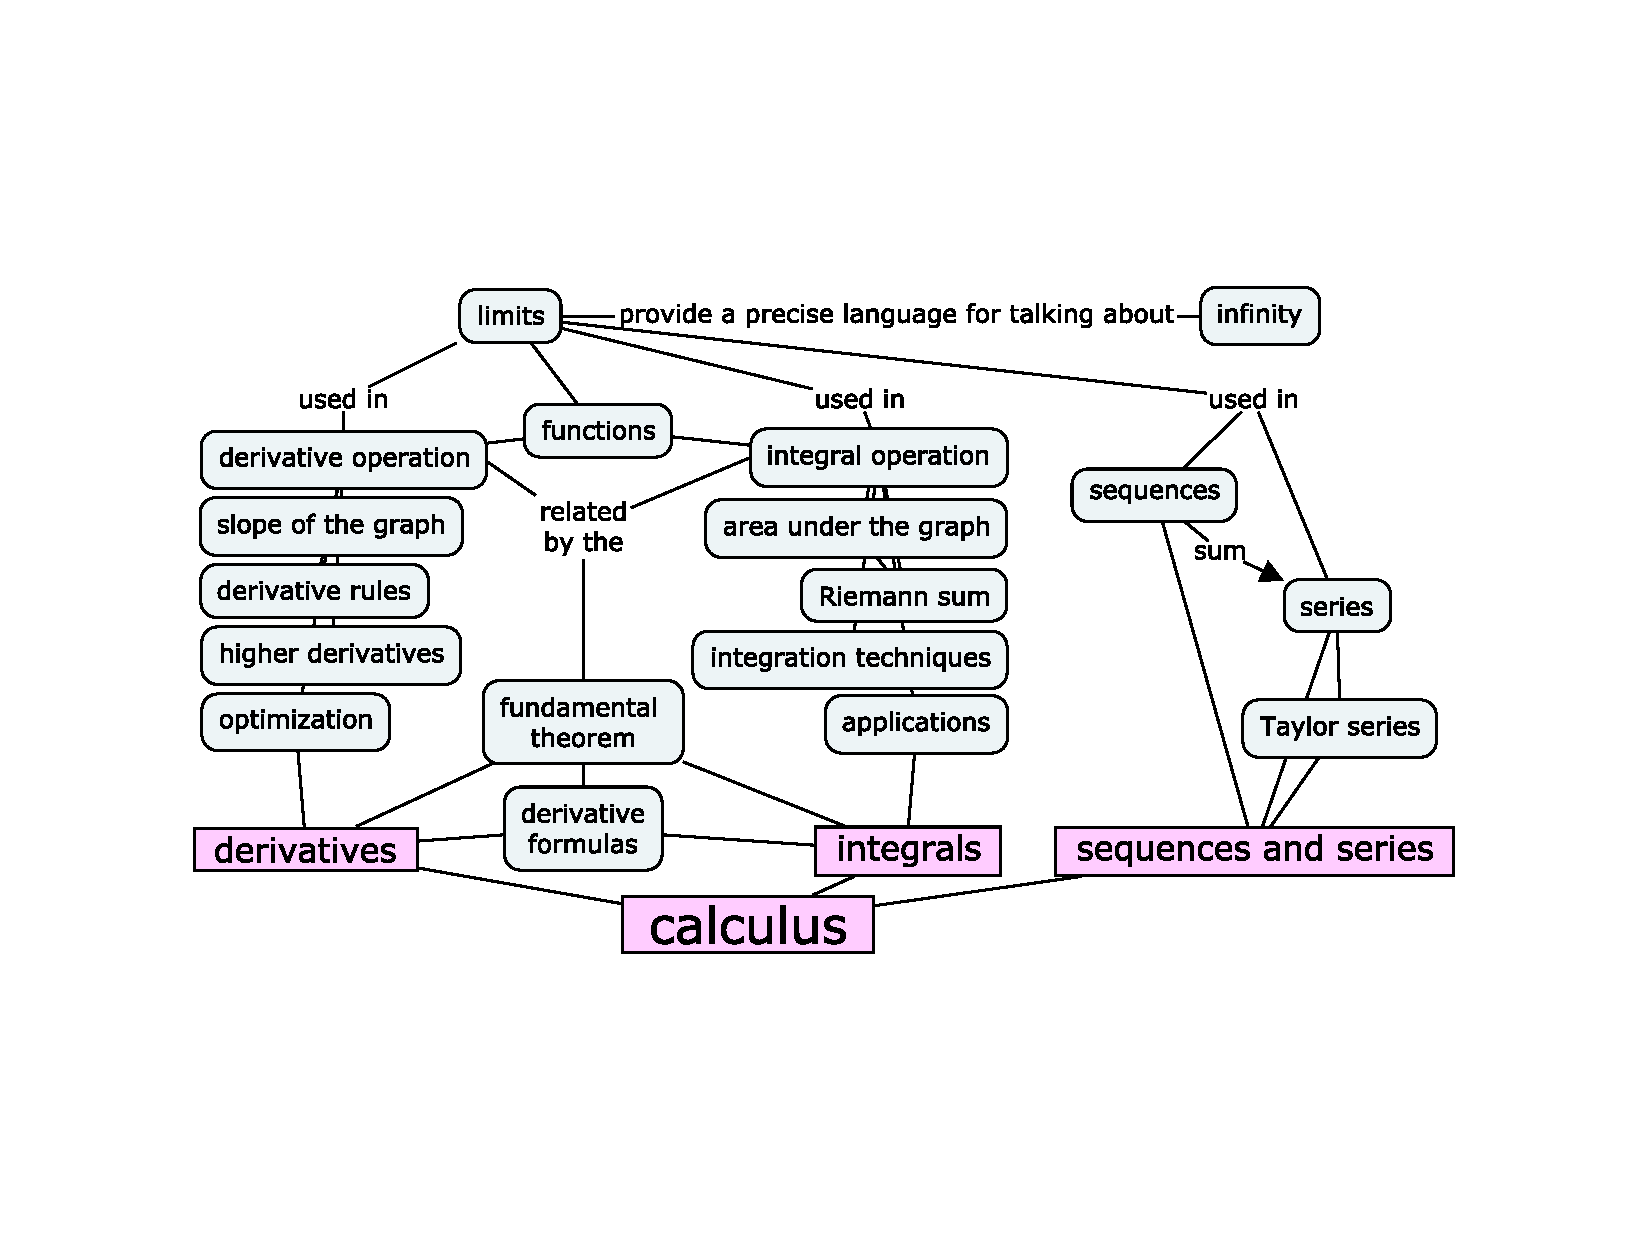
\includegraphics[width=0.99\columnwidth]{figures/calculus/calculus_tutorial_overview.pdf}%
		\vspace{-2mm}
		\caption{	The calculus concepts and topics you'll learn in this tutorial.}
		\label{fig:calculus_tutorial_overview}
	\end{figure}

	We'll start % theis tutorial
	by introducing limits in Section~\ref{sec:limits}.
	Limits give us a precise language to talk about infinity.
	% ALT: talk about infinitely large and infinitely small quantities
	Limits are a cornerstone idea in calculus,
	because they allow us to define the calculus operations:
	derivatives, integrals, and series.
	%
	We'll discuss derivatives 
	in Section~\ref{sec:derivatives}
	and integrals in Section~\ref{sec:integrals}.
	We'll then talk about sequences and series
	in Section~\ref{sec:sequences_and_series},
	and conclude with a brief intro to multivariable calculus in Section~\ref{sec:multivariable_calculus}.

	Throughout the tutorial,
	we'll explain concepts using text, formulas, graphs, and code examples.
	My intention is for you to understand the key ideas of calculus in theory,
	but also learn practical skills you can use to solve real-world problems.




%  LIMITS  %%%%%%%%%%%%%%%%%%%%%%%%%%%%%%
%\clearpage
%!TEX root = ../calculus_tutorial.tex

\section{Limits}
\label{sec:limits}

	Limits are a precise mathematical language for talking about
	infinitely large numbers,
	infinitely small lengths,
	and procedures with an infinite number of steps.
	We use the shorthand ``$\lim$'' to denote limit expressions.
	For example,
	the expression $\lim_{x \to \infty} f(x)$,
	read ``the limit of $f(x)$ as $x$ goes to infinity,''
	describes what happens to $f(x)$ when the input to the function $x$ tends to infinity (gets larger and larger).


	\subsection{Example: Archimedes' approximation to $\pi$}
	% ALT. Archimedes' approximation for area of a circle

		We'll start by looking at a visual example of a math procedure
		% with infinite number of steps
		that was invented by Archimedes of Syracuse around 250 BCE.
		Archimedes wanted to calculate the area of a circle of radius $r=1$.
		Today we know the formula for the are of the circle is $A_{\circ} = \pi r^2$,
		so the area of a circle with radius $r=1$ is $\pi$,
		but try to place yourself in Archimedes's shoes (sandals?)
		and suppose that you don't know the formula yet.

		Archimedes' clever idea was to approximate the circle
		as a regular polygon with $n$ sides inscribed in the circle.
		Figure~\ref{fig:inscribed-hexagon-octagon-dodecagon}
		shows the hexagonal (6-sides),
		octagonal (8-sides),
		and dodecagonal (12-sides) approximations to the circle.

		\begin{figure}[htb]
			\centering
			\includegraphics[width=0.99\columnwidth]{figures/calculus/inscribed-polygons.pdf}%
			\vspace{-3mm}
			\caption{	Approximations to the area of circle using a hexagon,
					an octagon, and a dodecagon inscribed inside a circle of radius $r$.}
			\label{fig:inscribed-hexagon-octagon-dodecagon}
		\end{figure}

		Archimedes computed the area of the $n$-sided regular polygons
		by splitting it up into $2n$ triangular slices,
		like the one shown in Figure~\ref{fig:inscribed-hexagon-octagon-dodecagon}~(b).
		He then compute the area each slice using the formula for the area of a triangle,
		and added up the areas of these $2n$ triangles
		to obtain the total area of the $n$-sided polygon.
		Let's denote $A(n)$ the area approximation
		computed from a $n$-sided polygon.
		Looking at Figure~\ref{fig:inscribed-hexagon-octagon-dodecagon},
		we see the approximations to the area of the circle
		using six-sided and eight-sided polygons are underestimates for the total area.
		However,
		the polygon with $n=12$ is starting to look like a circle,
		and we can use our imagination to see that the approximation $A(n) \approx A_{\circ}$
		will get more and more accurate as $n$ becomes larger and larger.
		Archimedes computed an approximation using a $n=96$ sided polygon,
		but thanks to computers we can push the approximation to much higher values of $n$.
		For example,
		using a 50-sided polygon gives us $A(50) = 3.1\ldots$.
		The approximation with $n=1000$ is accurate to four decimals $A(1000) = 3.1415\ldots$,
		and using $n=10K$ we get an approximation to $\pi$
		that is accurate to six decimals $A(10000) = 3.141592\ldots$.
		See the computational notebook here for the details of the calculations:
		\href{https://bit.ly/calctut3}{\tt{bit.ly/calctut3}}.

		In the limit as $n \to \infty$, 
		the $n$-sided-polygon approximation to the area of the circle 
		will becomes \emph{exactly} equal to $\pi = 3.141592653589793\ldots$,
		which we write as $\lim_{n \to \infty} A(n) = \pi$.
		Note that $A(n) \neq \pi$ for any finite number $n$ no matter how large.
		It is only in the limit as $n$ goes to infinity that the approximation becomes exact.

	\medskip
	\noindent
	Let's look at another example of a simple math procedure with $n$ steps
	that produces an important number when $n$ goes to infinity.
	% ALT.  that allows us to compute an important number 


	\subsection{Example: Euler's number}
	\label{introduction:eulers_number}

		Suppose you take out a loan with 100\% nominal interest rate.
		This is a very bad loan that nobody would agree to the real world,
		but we'll use it for this example to make the math come out simpler.
		An interest of $100\%$ calculated yearly means at the end of one year,
		you'll owe $(1+100\%) = (1+1)=2$ times the amount you borrowed initially.

		However,
		most banks don't calculate the interest owed only once per year,
		but more often.
		If the bank calculates the interest twice per year,
		during the first six months you'll have accrued $\frac{100\%}{2} = 50\%$ of interest,
		so you'll owe them $(1+50\%) = (1+\frac{1}{2}) = 1.5$ times the initial amount.
		Then during the second six months,
		the amount owed will grow by an additional $(1+50\%) = (1+\frac{1}{2}) = 1.5$,
		so at the end of the year,
		you'll owe $(1+\frac{1}{2})(1+\frac{1}{2}) = 2.25$.

		If the bank computes the interest three times per year,
		the amounted owed after one year is $(1+\frac{1}{3})(1+\frac{1}{3})(1+\frac{1}{3}) = 2.370$.
		If they compute the interest four times per year (quarterly),
		then you'll owe $(1+\frac{1}{4})(1+\frac{1}{4})(1+\frac{1}{4})(1+\frac{1}{4})  = 2.441$.
		Note the amount owed after one year keeps changing,
		as the compounding is performed more frequently.
		In general,
		when the compounding is performed $n$ times per year,
		the amount owed at the end of the year will be
		\[
			\underbrace{
			\left(1 + \tfrac{1}{n} \right)
			\left(1 + \tfrac{1}{n} \right)
			\cdots
			\left(1 + \tfrac{1}{n} \right)
			}_{n \text{ times}}
			= 
			\left(1 + \tfrac{1}{n} \right)^{\!n}.
		\]

		\noindent
		With monthly compounding ($n=12$),
		the amount owed will be $(1 + \tfrac{1}{12})^{12} = 2.613$
		at the end of one year.
		With daily compounding,
		the amount would be $(1 + \tfrac{1}{365})^{365} = 2.715$.
		If computing the interest $n=1000$ times per year,
		the amount ill be $(1 + \tfrac{1}{1000})^{1000} = 2.717$.
		The amount owed keeps increasing,
		but it seems to ``stabilize'' around the value $2.71$.

		What happens if we perform the compounding even more frequently?
		Specifically,
		we want to know what happens if the compound interest interest is calculated infinitely often.
		The infinitely-often calculation corresponds
		to computing the \emph{limit} of expression  $(1 + \frac{1}{n})^n$,
		as $n$ goes to infinity,
		which is written as follows using math notation:
		\[
			\lim_{n\to \infty} \left( 1 + \tfrac{1}{n}\right)^{\!n}
				\;\; = \;\; e
				\;\;= \;\; 2.718281828\ldots.
		\]
		This limit expression \emph{converges} to the value $e = 2.71828\ldots$,
		which is known as \emph{Euler's number}.
		% The number $e$ describes the limit of the annual growth rate of a loan
		If we borrow $\$1000$,
		we'll owe $\$1000e = \$2718.28$ at the end of one~year.		
		%	 compound interest calculation for an annual interest rate of $100\%$
		%	with compounding is performed infinitely often.


	We defined the number $\pi$ as the limit $\lim_{n \to \infty} A(n)$
	and the number $e$ as the limit $\lim_{n\to \infty} \left( 1 + \tfrac{1}{n}\right)^{\!n}$.
	These definition of the numbers $\pi$ and $e$ using as limits
	are go beyond the regular math operations we learn in high school math.
	The limit expression $\lim_{n \to \infty}$ doesn't describer any particular number $n$,
	but the \emph{process} of plugging in large and larger values of $n$.
	% This is what the limit notation $\lim_{n\to \infty} (1 + \frac{1}{n})^n$ means:
	% it describes the behaviour of the expression $(1 + \frac{1}{n})^n$
	% as $n$ goes to infinity.


% TODO: summarize + drive point home => procedures 
%	$\displaystyle  \lim_{n \to \infty} \textrm{proc}(n)$:
%	limit expression that describes the outcome of some computational procedure with $n$ steps,
%	as the number of steps $n$ goes to infinity.
% The parameter $n$ usually describes the number of steps in a given procedure,
% and $\textrm{proc}(n)$ describes the output of this procedure when $n$ steps are used.


		% EULER'S NUMBER VIA SERIES	
		%	Euler's number $e$ can also be obtained from another limit expression:
		%	\[
		%		e	=	1  + 1 + \frac{1}{2!} + \frac{1}{3!} + \frac{1}{4!}  + \cdots
		%			= 	\lim_{n\to \infty} \sum_{k=0}^n \frac{1}{k!}
		%			= 	2.718281828\ldots.
		%	\]
		%	This alternative expression
		%	tells us we can compute $e$ as the sum ($\sum$)
		%	with an infinite number of terms.
		%	Each term comes from a common ``pattern'' $\frac{1}{k!}$,
		%	where $k! = k\!\cdot\!(k-1) \cdots 3\!\cdot\!2\!\cdot\!1$
		%	is the factorial function.
		%	The notation $\sum_{k=0}^n$
		%	describes the summation starting at $k=0$ and going all the way to $k=n$.
		%	The limit $\lim_{n\to \infty}$ tells us the summation has infinitely many terms.
		%	This kind of infinite sum expression are called a \emph{series},
		%	and provides a powerful way to compute quantities by summing together a bunch of terms.
		%	We'll learn more about sequences and series in Section~\ref{sec:sequences_and_series}.







	\subsection{Limits at infinity}
	\label{limits:limits_to_infinity}

		We can use limit expressions to describe
		what happens to a certain function when its input variable tends to infinity.
		Does $f(x)$ approach a finite number,
		or does it keep growing to $\infty$?
		The function $f(x)$ is said to \emph{converge} to $L$
		if the function approaches the value $L$ for large values of $x$:
		\[
			\lim_{x \to \infty} f(x)  =  L.
		\]
		We say ``the limit of $f(x)$ as $x$ goes to infinity is $L$.''
		See Figure~\ref{fig:limit-at-infinity-graph} for an illustration.
		% ALT.
		%	The limit equation $\displaystyle \lim_{x \to \infty} f(x) = L$
		%	states that the  ``limit at infinity'' of the function $f(x)$ is equal to the number $L$.

		\begin{figure}[htb]
			\centering
			\includegraphics[width=0.63212\columnwidth]{figures/calculus/limit-at-infinity-graph.png}
			\vspace{-3mm}
			\caption{	A function $f(x)$ that oscillates up and down initially,
					but  it ``settles down'' close to the value $L$ for large values of $x$.}
			\label{fig:limit-at-infinity-graph}
		\end{figure}


		\subsubsection{Example 1}

			Consider the limit of the function $f(x) = \frac{1}{x}$ as $x$ goes to infinity,
			as illustrated in Figure~\ref{fig:limits_examples}~(a):
			\[
				\lim_{x \to \infty} f(x)
					= 	\lim_{x \to \infty} \tfrac{1}{x}
					= 	0.
			\]
			The function $\tfrac{1}{x}$ never \emph{actually} reaches zero,
			so it would be wrong to write $f(x)=0$ for any $x \in \mathbb{R}$.
			However,
			the expression $\frac{1}{x}$ gets closer and closer to $0$ as $x$ goes to infinity.
			Limits are useful because they allow us describe this tendency as $\displaystyle \lim_{x\to \infty} f(x)=0$.
			% even though $f(x)\neq 0$ for any number $x$.



		\begin{figure}[htb]
			\centering
			\includegraphics[width=0.99\columnwidth]{figures/calculus/limits_examples.pdf}
			% TODO: redo figure with xmax=8
			\vspace{-6mm}
			\caption{	Visual representation of the limit calculations for three functions.}
					%	$\lim_{x\to \infty} \frac{1}{x}$,
					%	$\lim_{x\to \infty} \frac{2x+1}{x}$,
					%	$\lim_{x\to 0^-} H(x)$, and $\lim_{x\to 0^+} H(x)$.}
			\label{fig:limits_examples}
		\end{figure}



		%	% CUTTABLE
		%	The limit expression is a concise way of saying the following precise mathematical statement:
		%	\begin{multline*}
		%	  \textrm{For all } \epsilon>0,
		%	  	 \textrm{ there exists a number } S \textrm{ such that } \\ 
		%		 	\left|f(x) - L\right| <\epsilon
		%			\textrm{ for all } x \textrm{ greater than or equal to } S.
		%	\end{multline*}
		%
		%	\noindent
		%
		%	You can think of this fancy statement
		%	as a formal way that a mathematician can prove $\displaystyle \lim_{x \to \infty} f(x) = L$ is true.
		%	You tell the mathematician a level of $\epsilon$ that would convince you,
		%	and the mathematician must find a starting point~$S$
		%	after which $f(x)$ becomes (and stays) $\epsilon$-close to the limit $L$.
		%	If the mathematician can succeed for all levels of precision $\epsilon$,
		%	not matte show small,
		%	then we have to believe that $\displaystyle \lim_{x \to \infty} f(x) = L$ is true.
		%	% /CUTTABLE


	\subsection{Limit formulas}

		The limit of the sum, difference, product, and quotient of two functions
		are can be computed as follows:
		% is equal to the corresponding operation of the limits of the two functions:
		\begin{align*}	
			\lim_{x \to \infty} (f(x) + g(x)) 	& =  \lim_{x \to \infty} f(x) + \lim_{x \to \infty} g(x), 	\\
			\lim_{x \to \infty} (f(x) - g(x)) 	& =  \lim_{x \to \infty} f(x) - \lim_{x \to \infty} g(x), 	\\
			\lim_{x \to \infty} f(x)g(x) 		& =   \lim_{x \to \infty} f(x) \cdot \lim_{x \to \infty} g(x), \\
			\lim_{x \to \infty} (f(x) / g(x)) & =  \lim_{x \to \infty} f(x) \, / \lim_{x \to \infty} g(x) \, .
			% \lim_{x \to \infty} \frac{f(x)}{g(x)} & =  \frac{ \displaystyle \lim_{x \to \infty} f(x) } { \displaystyle \lim_{x \to \infty} g(x)} \, .
		\end{align*}

		\noindent
		In words,
		these formulas tell us we
		can bring the limit calculations ``inside'' basic arithmetic operations.


		\subsubsection{Example 2}

			Calculate $\lim\limits_{x\to \infty} \frac{2x+1}{x}\,$.
			We're given the function $f(x)=\frac{2x+1}{x}$
			and must determine what the function looks like for very large values of $x$.
			We can rewrite the function as $\frac{2x+1}{x}=2+\frac{1}{x}$
			then apply the sum formula for limits:
			\[
				\lim_{x\to \infty}\!\! \tfrac{2x+1}{x} 
					= \lim_{x\to \infty}\!\left( 2 + \tfrac{1}{x} \right)
					= \lim_{x\to \infty} 2 + \!\lim_{x\to \infty} \tfrac{1}{x} 
					= 2 + 0 = 2.
			\]
			As the denominator $x$ becomes larger and larger,
			the fraction $\frac{1}{x}$ becomes smaller and smaller,
			so $\displaystyle \lim_{x \to \infty} \tfrac{1}{x} = 0$,
			so the second term goes zero,
			leaving only the $2$.
			See Figure~\ref{fig:limits_examples}~(b) for an illustration.



	\subsection{Limits to zero}
	\label{limits:limits_to_zero}

		The limit expression $\lim_{x \to 0} f(x)$
		describes the behaviour of the function $f$ for infinitely small values of $x$.
		The limit $\lim_{x \to 0} f(x)$,
		read ``the limit of $f(x)$ as $x$ goes to zero,''
		asks us to evaluate the function $f$ for inputs like
		$x=0.1$, $x=0.01$, $x=0.001$, $x=0.0001$, etc.
		to see the behaviour of the function for very small values of $x$.

		For example,
		the limit $\lim_{x \to 0} \frac{1}{x} = \infty$.
		In words,
		the function $f(x) = \frac{1}{x}$ ``blows up'' to infinity as $x$ goes to $0$.
		See Figure~\ref{fig:limits_examples}~(a).


	\subsection{Limits to a number}
	\label{limits:limits_to_a_number}

		More generally,
		the limit of $f(x)$ approaching $x=a$ \emph{from the right}
		is denoted $\lim_{x\to a^+} f(x) = \lim_{\delta \to 0} f(a + \delta)$.
		We use the symbol $\delta$ (the Greek letter \emph{delta}) to describes a distance
		that gets smaller and smaller.
		This limit expression that describes the value of the function $f$
		as the input $x$ gets closer and closer to $a$
		with values like $a+0.1$, $a+0.01$, $a+0.001$, $a+0.0001$, etc.
		%
		The limit of $f(x)$ when $x$ approaches \emph{from the left} is defined analogously,
		$\lim_{x\to a^-} f(x)  = \lim_{\delta \to 0} f(a - \delta)$.
		%		describes what happens to $f(x)$ as $x$ approaches $a$ from below
		%		(from the left) with values like $x=a-$, 
		%		with $\delta>0, \delta \to 0$.

		If both limits from the left and from the right at $x=a$
		exist and are equal to each other,
		we say the limit as $x\to a$ exists:
		\[
			\lim_{x\to a} f(x) =  \lim_{x\to a^+} f(x) =  \lim_{x\to a^-} f(x).
		\]
		For the two-sided limit of a function to exist at a point,
		both the limit from the left and the limit from the right must converge to the same number.










	\subsection{Continuity}
	\label{limits:continuity}

		If the function $f(x)$ obeys, $f(a) = L$ and $\lim_{x\to a} f(x) = L$,
		we say the function $f(x)$ is \emph{continuous} at $x=a$.
		Geometrically,
		the graph of the continuous function at $x=a$ is ``smooth'' curve
		that doesn't have any hole or a jump at $x=a$.
		Intuitively,
		when a function is continuous,
		we can draw its graph using a single pen stroke
		without lifting the pen.
		% means the function's graph looks like a smooth curve
		In contrast,
		functions that blow up to infinity or make sudden jumps are not continuous.

		\subsubsection{Example 3}

			The \emph{Heaviside step function} is an example of a function
			with a jump discontinuity.
			It is defined as follows:
			\[
				H(x) \eqdef \begin{cases}
							\; 1, 	& \text{if } x \geq 0 \\
							\; 0, 	& \text{if } x < 0.
						\end{cases}
			\]

			\noindent
			The function is zero for negative values of $x$,
			then suddenly jumps to one at $x=0$,
			as shown in Figure~\ref{fig:limits_examples}~(c).
			The limit as $x$ approaches $x=0$ from the left is $\lim_{x\to 0^-} H(x) = 0$.
			The limit at $x=0$ from the right is $\lim_{x\to 0^+} H(x) = 1$.
			The two limits are different,
			$\lim_{x\to 0^-} H(x) = 0 \neq 1 = \lim_{x\to 0^+} H(x)$,
			so the function is \emph{discontinuous} at $x=0$.


		%	A more mathematically precise way to define continuity is to say the function is equal to its limit for all $x$.
		%	We say a function $f(x)$ is \emph{continuous} at $a$ if the limit of $f$ as $x\to a$ converges to $f(a)$:
		%	\[
		%	 \lim_{x \to a}  f(x) =  f(a).
		%	\]
		%	Remember,
		%	the two-sided limit $\lim_{x\to a}$ requires both the left and the right limit to exist and to be equal.
		%	Thus, the definition of continuity implies the equality $\lim_{x \to a^-}  f(x) =  f(a)$
		%	and $f(a) = \lim_{x \to a^+}  f(x)$,
		%	which correspond to the idea of ``not lifting the pen'' when drawing the graph at $x=a$.

		%	In words,
		%	this means that a function $f(x)$ is continuous at $x=a$
		%	if the limit from the left $\lim_{x \to a^-}  f(x)$
		%	and the limit from the right $\lim_{x \to a^+}  f(x)$
		%	are both equal to the value of the function at $x=a$.
		%	% Take a moment to think about the mathematical definition of continuity at a point.
		%	% Can you connect the math definition to the intuitive idea
		%	% that functions are continuous if they can be drawn without lifting the pen?
		%	Most functions we'll study in calculus are continuous,
		%	but not all functions are.

		%	Functions that are not defined for some value, as well as functions that make sudden jumps, are not continuous.
		%	%		Another examples is the function $f(x)=\frac{2x+1}{x}$ which is discontinuous at $x=0$
		%	%		(because the limit $\lim_{x \to 0}  f(x)$ doesn't exist and $f(0)$ is not defined).
		%	For example,
		%	consider the function $f : \mathbb{R} \setminus \{0\} \to \mathbb{R}$ defined by
		%	\[
		%		f(x)
		%		=\frac{ | x-3| }{x-3} 
		%		= \left\{ 	\begin{array}{rl}
		%				1	\quad	&  \mathrm{  if } \;  x > 3, \\
		%				-1	\quad	&  \mathrm{  if } \;  x < 3.
		%		                        \end{array}                    \right.
		%	\]
		%	The function $f$ is continuous everywhere on the real line except at $x=3$.
		%	Since this function $f$ is ``missing'' only at a single point,
		%	we can try to ``patch it'' by filling in the missing value.
		%	Consider the function $g : \mathbb{R} \to \mathbb{R}$ defined as
		%	\[
		%		g(x)
		%		= \left\{ 	\begin{array}{rl}
		%				1	\quad	&  \mathrm{  if }\;  x > 3, \\
		%				1	\quad	&  \mathrm{  if }\;  x = 3, \\
		%				-1	\quad	&  \mathrm{  if } \;  x < 3.
		%		                        \end{array}                    \right.		
		%	\]
		%	The function $g$ is \emph{continuous from the right} at the point $x=3$,
		%	since $\lim_{x \to 3^+} g(x)=1=g(3)$.
		%	However,
		%	taking the limit from the left,
		%	we find $\lim_{x \to 3^-} g(x)=-1 \neq g(3)$,
		%	which tells us $g$ is not continuous from the left.
		%	We say the function $g$ has a \emph{jump discontinuity} at $x=3$.

		% Khan Academy
		% https://www.youtube.com/watch?v=Y7sqB1e4RBI

		%	\paragraph{Example 3}	
		%		We can calculate the limit $\displaystyle\lim_{x\to 5} \frac{2x+1}{x}$ as follows:
		%		\[
		%		 \lim_{x\to 5} \frac{2x+1}{x}
		%		  = \frac{2(5)+1}{5}
		%		  = \frac{11}{5}.
		%		\]
		%		There is nothing tricky going on here---we plug the number $5$ into the equation, and voila. 
		%		The function $f(x)=\frac{2x+1}{x}$ is continuous at the value $x=5$, so the limit of the function 
		%		as $x\to 5$ is equal to the value of the function $\displaystyle\lim_{x\to 5} f(x) = f(5)$.
		%		% This is true in general for any continuous function.





	\subsection{Computing limits using SymPy}
	
		We can use SymPy to compute limit expression,
		which allows us to check the answers we obtain using pen-and-paper calculations.
		We'll start by importing the \tt{sympy} module under the alias \tt{sp},
		defining the symbolic variable $\tt{n} = n$,
		which we can then use to write various expressions.

		\begin{codeblock}[sympy-e-from-limit]
		>>> import sympy as sp
		>>> n = sp.symbols("n")
		\end{codeblock}

		To compute limits,
		we use the SymPy function \tt{sp.limit(expr,var,value)},
		which computes the limit of the expression \tt{expr},
		as the variable \tt{var} approaches \tt{value}.
		For limits toward infinity,
		we use the special symbol \texttt{sp.oo} (two lowercase \texttt{o}s),
		which is a clever name chosen because it resembles the infinity symbol $\infty$.

		% We can use SymPy to check the limit calculation we saw above.		
		% EXAMPLE  e
		Euler's number is defined as the limit
		$e \eqdef \lim_{n\to \infty} \left( 1 + \frac{1}{n}\right)^{n}$.
		To compute this limit using SymPy,
		we call \tt{sp.limit} on the expression \tt{(1+1/n)**n}
		as $\tt{n}$ goes to infinity $\infty = \texttt{sp.oo}$:

		\begin{codeblock}[sympy-e-from-limit]
		>>> sp.limit((1+1/n)**n, n, sp.oo)
		E
		>>> sp.limit((1+1/n)**n, n, sp.oo).evalf(40)
		2.718281828459045235360287471352662497757
		\end{codeblock}

		\noindent
		The result of \tt{sp.limit} is the exact value $e$
		which is represented symbolically as \tt{E}.
		On the second line,
		we used the method \tt{.evalf(40)} 
		to compute an approximation to $e$ to 40 decimals.


		% EXAMPLE 1/x
		Let's now compute the limits $\lim_{x \to \infty} \tfrac{1}{x}$
		and $\lim_{x \to 0^+} \tfrac{1}{x}$.
		We fist define the symbol \tt{x}
		then call the function \tt{sp.limit} to evaluate the two limits
		involving the expression $\tt{1/x} = \frac{1}{x}$:

		\begin{codeblock}[]
		>>> x = sp.symbols("x")
		>>> sp.limit(1/x, x, sp.oo)
		0
		>>> sp.limit(1/x, x, 0)
		oo
		\end{codeblock}

		\noindent
		SymPy confirms that $\lim_{x \to \infty} \tfrac{1}{x} = 0$
		and $\lim_{x \to 0^+} \tfrac{1}{x} = \infty$,
		as calculated earlier.
		See Figure~\ref{fig:limits_examples}~(a) for an illustration.


		% EXAMPLE (2x+1)/x		
		Here is another example,
		that computes the limit of the fraction $\frac{2x+1}{x}$ as $x$ goes to infinity,
		which is illustrated in Figure~\ref{fig:limits_examples}~(b).

		\begin{codeblock}[]
		>>> sp.limit((2*x+1)/x, x, sp.oo)
		2
		\end{codeblock}

		% EXAMPLE  Heaviside
		\noindent
		To calculate the limit form the left and the right of a number,
		we must provide a fourth argument \tt{"-"} or \tt{"+"}.
		The following SymPy calculations confirm the limits of the Heaviside step function
		when approaching $x=0$ from the left and from the right.

		\begin{codeblock}[]
		>>> from sympy import Heaviside
		>>> sp.limit(Heaviside(x,1), x, 0, "-")
		0
		>>> sp.limit(Heaviside(x,1), x, 0, "+")
		1
		\end{codeblock}

		\noindent
		See Figure~\ref{fig:limits_examples}~(c) for an illustration.


		% TODO: ADD MORE LIMIT EXAMPLES
		%	Here are some other examples of limits:

		% NOTEBOOK ONLY
		%	Infinity is not a number but a process: the process of counting forever.
		%	Thus, $\infty + 1 = \infty$, $\infty$ is greater than any finite number, and $1/\infty = 0$.
		%	\begin{codeblock}[]
		%	>>> from sympy import oo
		%	>>> oo+1
		%	oo
		%	>>> 5000 < oo 
		%	True
		%	>>> 1/oo
		%	0
		%	\end{codeblock}

		% BONUS SYMPY EXAMPLES
		%	The SymPy function \tt{limit} allows us to compute limit expressions.
		%	For example,
		%	if we want to see if the exponential function $e^x$ or the polynomial function $x^{100}$ grows faster
		%	in the limit as $x$ goes to infinity,
		%	The code for computing the limit of the ratio between these two expressions is
		%
		%	\begin{codeblock}[sympy-limit-exp-over-x-100]
		%	>>> from sympy import limit, exp, oo
		%	>>> limit(exp(x)/x**100, x, oo) 
		%	oo
		%	\end{codeblock}
		%
		%	\noindent
		%	The answer $\infty$,
		%	written as \tt{oo} (two lowercase letters ``o''),
		%	tells us exponential functions grow faster than polynomial functions.
		%	%	This result has implications in computer science,
		%	%	where algorithms whose running time grows exponentially with the size of their input are considered bad





	\subsection{Applications of limits}

		Limits are important because they are used in the formal definitions of derivatives, integrals, and series:

		\begin{itemize}

			\item The derivative function $f^{\prime\!}(x)$
				describe the instantaneous rate change of the function $f(x)$.
				In Section~\ref{sec:derivatives} we'll learn how to calculate derivatives
				by evaluating a limit of the form $\lim_{\delta \to 0}$.

			\item The integral $\int_a^b f(x) \, dx$
				describes the area under the graph of the function $f(x)$ between $x=a$ and $x=b$.
				In Section~\ref{sec:integrals}
				we'll learn how to compute integrals by splitting up area into $n$ rectangular strips
				and taking the limit $\lim_{n \to \infty}$.

			\item The series $\sum_{k=1}^n a_k$ describes
				the sum of all the first $n$ terms in the sequence $a_k$.
				In Section~\ref{sec:sequences_and_series},
				we'll learn how to compute infinite series by taking $\lim_{n \to \infty}$.

		\end{itemize}


% Many important math and science quantities are defined as limit expressions.

% LEAD OUT	
%	In the remainder of this tutorial we'll use limits to evaluate derivatives, integrals, and series expressions.
%	In each of these domains,
%	limit expressions will help us make precise statements
%	that describe calculus procedures with infinite small lengths and infinite number of steps.









% TODO: Limit exercises








% \subsubsection{Example: split up line}
%		Let's begin with a simple example.
%		Say you have a string of length $\ell$ and you want to divide it into infinitely many, infinitely short segments.
%		There are infinitely many segments,
%		and they are infinitely short, so together the segments add to the string's total length $\ell$.
%
%		It's easy enough to describe this process in words.
%		Now let's describe the same process using the notion of a limit.
%		If we divide the length of the string $\ell$ into $N$ equal pieces then each piece will have a length of
%		\[
%		   \delta = \frac{\ell}{N}  \,.
%		\]
%		Let's make sure that $N$ pieces of length $\delta$ added together equal the string's total length: 
%		\[
%		 N \delta = N \frac{\ell}{N} = \ell.
%		\]
%		
%		\noindent
%		Now imagine what happens when the variable $N$ becomes larger and larger.
%		The larger $N$ becomes, the shorter the pieces of string will become.
%		In fact, if $N$ goes to infinity (written $N \to \infty$),
%		then the pieces of string will have zero length:
%		\[
%		 \lim_{N\to \infty}  \delta = \lim_{N\to \infty} \frac{\ell}{N} = 0.
%		\]
%		In the limit as $N \to \infty$, the pieces of string are \emph{infinitely small}.
%		
%		Note we can still add the pieces of string together to obtain the whole length:
%		\[
%		 \lim_{N\to \infty}  \left( N \delta \right) 
%		 = 
%		 \lim_{N\to \infty}  \left( N \frac{\ell}{N} \right)
%		 = \ell.
%		\]
%		Even if the pieces of string are \emph{infinitely small},
%		because there are \emph{infinitely many} of them,
%		they still add to $\ell$.
%
%			splitting up an interval into $n$ segments, then making $n$ go to infinity
%			splitting with an infinite number of segments
%			\begin{codeblock}[sympy-limit-sement-zero-length]
%			>>> from sympy import limit, oo, summation
%			>>> delta = (b - a)/n
%			>>> limit(delta, n, oo)
%			0
%			\end{codeblock}
%		
%			\begin{codeblock}[sympy-limit-sements-add-to-interval]
%			>>> summation(delta, (i, 0, n-1))
%			b - a				
%			\end{codeblock}
%
%		The take-home message is that as long as you clearly define your limits,
%		you can use infinitely small numbers in your calculations.
%		The notion of a limit is one of the central ideas in this course.


% \input{sections/limits2.tex}

%  DERIVATIVES  %%%%%%%%%%%%%%%%%%%%%%%%%%%
%\clearpage
%!TEX root = ../calculus_tutorial.tex

\section{Derivatives}
\label{sec:derivatives}

	The \emph{derivative} function, denoted $f^{\prime\!}(x)$, $\frac{d}{dx}f(x)$, or $\frac{df}{dx}$,
	describes the \emph{rate of change} of the function $f(x)$.
	For example,
	the constant function $f(x)=c$ has derivative $f^{\prime\!}(x)=0$ since the constant function doesn't change.
	Geometrically,
	the derivative function describes the \emph{slope} of the graph of the function $f(x)$.
	The derivative of the line $f(x)=mx+b$ is $f^{\prime\!}(x)=m$,
	since the slope of this line is equal to $m$
	for all values of $x$.
	In general,
	the slope of a function is different at different values of~$x$,
	so mathematicians invented the notation $f^{\prime\!}(x)$
	for describing ``the slope of the function $f$ at $x$.''


% NOD
Consider the rise-over-run formula for calculating the slope of a function
applied to the points $(x,f(x))$ and $(x+\delta, f(x+\delta))$ on the graph of the function.
Figure~REF
shows the slopes calculated when $\delta = 0.1$, $\delta = 0.01$, and $\delta = 0.001$.


The average slope between ... and ...
is

TODO: figure

but what about the instantaneous slope at one instant?



	The derivative function $f^{\prime\!}(x)$
	is defined as the following limit expression:
	\[
		f^{\prime\!}(x) \eqdef \lim_{\delta \to 0} \frac{f(x+\delta)\ - \ f(x)}{\delta}\,.
	\]
	In words,
	this formula describes the general rise-over-run calculation for computing the slope of a line that connects
	the points $(x,f(x))$ and $(x+\delta, f(x+\delta))$,
	with the step-length $\delta$ becoming infinitely small.

	%	The definition of the derivative comes from the rise-over-run formula for calculating the slope of a line:
	%	\[
	%	  \frac{ \textrm{rise} } { \textrm{run} } = \frac{ \Delta y } { \Delta x } 
	%		=  \frac{y_f - y_i}{x_f - x_i} = 
	%		\frac{f(x+\delta)\ - \ f(x)}{x + \delta \  -\  x}.
	%	\]
	%	By making $\delta$ tend to zero in the above expression,
	%	we're performing a rise-over-run of the function $f(x)$ at a point.

	Geometrically,
	the derivative function tells us the slope of the graph of the function $f(x)$ for all values of $x$.
	Figure~\ref{fig:derivative_as_slope_xsq} shows the slope calculation for the function $f(x) = x^2$
	at two different locations: at $x=-0.5$ and at $x=1$.
	% the slope of the function is the same as the line passing through this point


	\begin{figure}[htb]
		\centering
		\includegraphics[width=0.99\columnwidth]{figures/calculus/derivative_as_slope_xsq.pdf}
		\caption{	The derivative of the function at $x=a$ is denoted $f^{\prime\!}(a)$ and describes the slope function at that point.}
		%	\caption{	The diagram illustrates how to compute the derivative of the function $f(x) = x^2$
		%			at three different points on the graph of the function.
		%			To calculate the derivative of $f(x)$ at $x=1$, 
		%			we can ``zoom in'' near the point $(1,\tfrac{1}{2})$ and 
		%			draw a line that has the same slope as the function.
		%	 	 	We can then calculate the slope of the line using a rise-over-run calculation,
		%			aided by the mini coordinate system that is provided.
		%			The derivative calculations for $x=-\tfrac{1}{2}$ and  $x=2$ are also shown.
		%			Note that the slope of the function is different for each value of $x$. 
		%			What is the value of the derivative at $x=0$?
		%			Can you find the general pattern?}
		\label{fig:derivative_as_slope_xsq}
	\end{figure}

% TODO: explain grid 

	%	Derivatives occur so often in math that people have devised many ways to denote them:
	%	\[
	%	    Df(x) =  f^{\prime\!}(x) =  \frac{d}{dx}f(x) = \frac{df}{dx} = \frac{dy}{dx} = \nabla f.
	%	\]
	%	Don't be fooled by this multitude of notations---all of them refer to the same concept.

	% TODO: mention the derivative is a function of the form $f': \mathbb{R} \to \mathbb{R}$.
	The derivative function $f^{\prime\!}(x)$ is a property of the function $f(x)$.
	Indeed, this is where the name \emph{derivative} comes from:
	$f^{\prime\!}(x)$ is not an independent function---it
	is \emph{derived} from the slope property of the original function $f(x)$.

	More generally,
	we can define the \emph{derivative operation},
	denoted $\frac{d}{dx}[\tt{<f>}]$,		% ALT. derivative operator $\frac{d}{dx}$
	which takes as input a function $f(x)$ and produces as output the derivative function $f^{\prime\!}(x)$.
	% which is a function of the form $f': \mathbb{R} \to \mathbb{R}$.
	% For each input $x_0$ the derivative function tells you the slope of $f(x)$ when $x=x_0$.
	Applying the derivative operation to the function
	is also called ``taking the derivative'' of a function.
	For example, 
	the derivative of the function $f(x) = x^2$ is the function $f^{\prime\!}(x) = 2x$.
	We can also describe this relationship as $(x^2)^{\prime} = 2x$
	or as $\tfrac{d}{dx}(x^2) = 2x$.
	Look at the graph in Figure~\ref{fig:derivative_as_slope_xsq} to convince yourself
	that the slope of $f(x)=x^2$ is indeed described by $f^{\prime\!}(x)=2x$ for any $x$.
	For example,
	when $x=0$,
	we see the graph has zero slope
	and the derivative gives us the same thing: $f^{\prime\!}(0) = 0$.


	\subsection{Numerical derivative calculations}

		Here is the Python code for computing
		a numerical approximations to the derivative the function \tt{f} at the point~\tt{x}:

		\begin{codeblock}[]
		>>> def differentiate(f, x, delta=1e-9):
		        df = f(x+delta) - f(x)
		        dx = delta
		        return df / dx
		\end{codeblock}

		\noindent
		The function \tt{differentiate} calculates the derivative using a finite step $\tt{delta} = 10^{-9}$
		instead of the infinitely small step $\delta$ in the math definition of the derivative.
		This means,
		the value returned by \tt{differentiate} will be an approximation to the true derivative.

		Let's now define a Python function \tt{f} that corresponds to the math function $f(x)=x^2$
		and use \tt{differentiate} to find the slope of $f$ when $x=1$:

		\begin{codeblock}[]
		>>> def f(x):
		        return x**2
		>>> differentiate(f, 1)
		2.000000165480742
		\end{codeblock}
		
		\noindent
		Using the numerical method,
		we obtain the approximation $f^{\prime\!}(1) = 2.000000165480742$,
		which is not perfect,
		but pretty close to the true value $f^{\prime\!}(1) = 2$.
		For most practical applications,
		this numerical approximation is good enough.

		%	The mathematical definition
		%	$f^{\prime\!}(x) \eqdef \lim_{ \delta \rightarrow 0}\frac{f(x+\delta)-f(x)}{\delta}$
		%	allows us to find a closed form expression for the derivative function
		%	that applies for all values of $x$.
		%	Finding the exact formula for the derivative requires a little bit more work upfront
		%	(to simplify an expressions that involves Greek symbols),
		%	but once you find the exact formula for the derivative $f^{\prime\!}(x)$,
		%	you can compute the slope of $f(x)$ at the point $x=c$
		%	by simply evaluating the the derivative function at that point:
		%	$f^{\prime\!}(c) = \{ \textrm{the slope of} \ f(x) \ \textrm{at} \ x=c\}$.



	\subsection{Derivative formulas}

		You don't need to apply the complicated derivative formula
		$f^{\prime\!}(x) \eqdef \lim_{\delta \to 0}\frac{f(x+\delta)-f(x)}{\delta}$
		every time you need to find the derivative of a function.
		For each function $f(x)$,
		it's enough to use the complicated formula once
		and record the formula you obtain for $f^{\prime\!}(x)$,
		then you can reuse that formula
		whenever you need to compute $f^{\prime\!}(x)$ in later calculations.

		Table~\ref{table:derivatives} shows the derivatives several functions.
		I invite you to mentally bookmark this page so you can come back to it
		when you need to know the derivatives of some function.

		\begin{table}[htb]
			\centering
			\caption{Derivative formulas for commonly used functions}
			\begin{shadebox}%
			\vspace{-2mm}
			\begin{align*}
			f(x)					&  \ -\textrm{derivative}\to  \   											f^{\prime\!}(x)		\\
			a					&\qquad  \raisebox{.52ex}{\rule{0.9em}{.4pt}}\;\tfrac{d}{dx} \rightarrow \qquad 		0		\\
			x					&\qquad  \raisebox{.52ex}{\rule{0.9em}{.4pt}}\;\tfrac{d}{dx} \rightarrow \qquad		1		\\
			mx+b				&\qquad  \raisebox{.52ex}{\rule{0.9em}{.4pt}}\;\tfrac{d}{dx} \rightarrow \qquad		m		\\
			x^n, \text{ for } n\neq 0	&\qquad  \raisebox{.52ex}{\rule{0.9em}{.4pt}}\;\tfrac{d}{dx} \rightarrow \qquad 		nx^{n-1}	\\
			\tfrac{1}{x} =  x^{-1}		&\qquad  \raisebox{.52ex}{\rule{0.9em}{.4pt}}\;\tfrac{d}{dx} \rightarrow \qquad 		\tfrac{-1}{x^2} = -x^{-2}	\\
			\sqrt{x} = x^{\frac{1}{2}}	&\qquad  \raisebox{.52ex}{\rule{0.9em}{.4pt}}\;\tfrac{d}{dx} \rightarrow \qquad
					\tfrac{1}{2\sqrt{x}} = \tfrac{1}{2}x^{-\frac{1}{2}}	\\
			e^x					&\qquad  \raisebox{.52ex}{\rule{0.9em}{.4pt}}\;\tfrac{d}{dx} \rightarrow \qquad 		e^x	\\
			\ln(x)					&\qquad  \raisebox{.52ex}{\rule{0.9em}{.4pt}}\;\tfrac{d}{dx} \rightarrow \qquad 		\tfrac{1}{x}		\\
			\sin(x)				&\qquad  \raisebox{.52ex}{\rule{0.9em}{.4pt}}\;\tfrac{d}{dx} \rightarrow \qquad 		\cos(x)		\\
			\cos(x)				&\qquad  \raisebox{.52ex}{\rule{0.9em}{.4pt}}\;\tfrac{d}{dx} \rightarrow \qquad 		-\sin(x)
			\end{align*}%
			\end{shadebox}
			\label{table:derivatives}
		\end{table}
%		\alpha f(x)+ \beta g(x)		&\qquad  \raisebox{.52ex}{\rule{0.9em}{.4pt}}\;\tfrac{d}{dx} \rightarrow \qquad 	\alpha f^{\prime\!}(x)+ \beta g^{\prime\!}(x)	\\
%	af(x)			&\qquad  \raisebox{.52ex}{\rule{0.9em}{.4pt}}\;\tfrac{d}{dx} \rightarrow \qquad 				af^{\prime\!}(x)		\\
%	f(x)+g(x)		&\qquad  \raisebox{.52ex}{\rule{0.9em}{.4pt}}\;\tfrac{d}{dx} \rightarrow \qquad 				f^{\prime\!}(x)+g^{\prime\!}(x)	\\
% a^x			&\qquad  \raisebox{.52ex}{\rule{0.9em}{.4pt}}\;\tfrac{d}{dx} \rightarrow \qquad 				a^x\ln(a)	\\
% \log_a(x)		&\qquad  \raisebox{.52ex}{\rule{0.9em}{.4pt}}\;\tfrac{d}{dx} \rightarrow \qquad 				(x\ln(a))^{-1}	\\
% \tan(x)			&\qquad  \raisebox{.52ex}{\rule{0.9em}{.4pt}}\;\tfrac{d}{dx} \rightarrow \qquad 				\sec^2(x) = \cos^{-2}(x)
%	\csc(x) = \frac{1}{\sin(x)}		&\qquad  \raisebox{.52ex}{\rule{0.9em}{.4pt}}\;\tfrac{d}{dx} \rightarrow \qquad 	-\sin^{-2}(x)\cos(x)	\\
%	\sec(x) = \frac{1}{\cos(x)}		&\qquad  \raisebox{.52ex}{\rule{0.9em}{.4pt}}\;\tfrac{d}{dx} \rightarrow \qquad 	\tan(x)\sec(x)	\\
%	\cot(x) = \frac{1}{\tan(x)}		&\qquad  \raisebox{.52ex}{\rule{0.9em}{.4pt}}\;\tfrac{d}{dx} \rightarrow \qquad 	-\csc^2(x)	\\
%	\sin^{-1}(x)		&\qquad  \raisebox{.52ex}{\rule{0.9em}{.4pt}}\;\tfrac{d}{dx} \rightarrow \qquad 				\frac{1}{\sqrt{1-x^2}}	\\
%	\cos^{-1}(x)		&\qquad  \raisebox{.52ex}{\rule{0.9em}{.4pt}}\;\tfrac{d}{dx} \rightarrow \qquad 				\frac{-1}{\sqrt{1-x^2}}	\\
%	\tan^{-1}(x)		&\qquad  \raisebox{.52ex}{\rule{0.9em}{.4pt}}\;\tfrac{d}{dx} \rightarrow \qquad 				\frac{1}{1+x^2}	\\
%	\sinh(x)		&\qquad  \raisebox{.52ex}{\rule{0.9em}{.4pt}}\;\tfrac{d}{dx} \rightarrow \qquad 				\cosh(x)	\\
%	\cosh(x)		&\qquad  \raisebox{.52ex}{\rule{0.9em}{.4pt}}\;\tfrac{d}{dx} \rightarrow \qquad 				\sinh(x)	

		\noindent
		Table~\ref{table:derivatives} presents the results
		in terms of the derivative operator $\frac{d}{dx}[\tt{<f>}]$,
		which takes as input some function $f(x)$
		and produces as output its derivative function $f^{\prime\!}(x)$.


	\subsection{Derivative rules}

		In addition to the table of derivative formulas,
		there are some important derivatives rules
		that allow you to find derivatives of \emph{composite} functions.

		\paragraph{Constant multiple rule}

			The derivative of $k$ times the function $f(x)$
			is equal to $k$ times the derivative of $f(x)$:
			\[
				\big[ k f(x) \big]^\prime		= 	k f^{\prime\!}(x).
			\]

		\paragraph{Sum rule}

			The derivative of the sum of two functions
			is the sum of their derivatives:
			\[
				\big[ f(x) +  g(x) \big]^\prime	=	f^{\prime\!}(x) + g^{\prime\!}(x).
			\]

			%	The derivative of a \emph{linear combination} of functions $\alpha f(x) + \beta g(x)$ is equal 
			%	to the same linear combination of the derivatives $\alpha f^{\prime\!}(x) + \beta g^{\prime\!}(x)$.


		\paragraph{Product rule}

			The derivative of a product of two functions
			is the sum of two contributions:
			\[
				\big[ f(x)g(x) \big]^\prime 		= 	f^{\prime\!}(x)g(x)  + f(x)g^{\prime\!}(x).
			\]
			In each term,
			the derivative of one of the functions
			is multiplied by the value of the other function.


		\paragraph{Quotient rule}

			This formula tells us how to obtain the derivative of a fraction of two functions:
			\[
				\left[ \frac{f(x)}{g(x)} \right]^\prime =	\frac{f^{\prime\!}(x)g(x)-f(x)g^{\prime\!}(x)}{g(x)^2}.
			\]
			
			
		\paragraph{Chain rule}
			If you encounter a situation that includes an inner function and an outer function,
			like $f(g(x))$, you can obtain the derivative by a two-step process:
			\[
				\big[ f(g(x)) \big]^\prime	= 	f^{\prime\!}(g(x))g^{\prime\!}(x).
			\]
			
			\noindent
			In the first step,
			we leave the inner function $g(x)$ alone
			and focus on taking the derivative of the outer function $f(x)$.
			This step gives us $f^{\prime\!}(g(x))$,
			which is the value of $f^{\prime}$ evaluated at $g(x)$.
			In the second step,
			we multiply this expression by the derivative of the \emph{inner} function $g^{\prime\!}(x)$.


	\subsection{Higher derivatives}

		The second derivative of $f(x)$ is denoted $f^{\prime\prime\!}(x)$ or $\frac{d^2f}{dx^2}$.
		It is obtained by applying the derivative operation to $f(x)$ \emph{twice}:
		$\frac{d}{dx}\big[ \frac{d}{dx}[\tt{<f>}] \big]$.
		Geometrically,
		the second derivative $f^{\prime\prime\!}(x)$
		tells us the \emph{curvature} of $f(x)$.
		Positive curvature means the function opens upward
		and looks like the bottom of a valley.
		The function $f(x)=x^2$ shown in Figure~\ref{fig:derivative_as_slope_xsq} 
		has derivative $f^{\prime\!}(x) = 2x$ and second derivative $f^{\prime\prime\!}(x) = 2$,
		which means it has positive curvature.
		Negative curvature means the function opens downward
		and looks like a mountain peak.
		For example,
		the function $g(x) = -x^2$ has negative curvature.


	\subsection{Examples}
	
		Armed with the derivative formulas from Table~\ref{table:derivatives} and the derivative rules from the previous section,
		you can the derivative of any function,
		no matter how complicated.
		Let's look at some examples.

		\paragraph{Example 1}
			To calculate the derivative of $f(x) = e^{x^2}$,
			we use the chain rule: $f^{\prime\!}(x) = e^{x^2}[x^2]'  = e^{x^2}2x$.

		\paragraph{Example 2}
			To find the derivative of $f(x) = \sin(x)e^{x^2}$,
			we use the product rule and the chain rule: $f^{\prime\!}(x) = \cos(x)e^{x^2} + \sin(x)2xe^{x^2}$.
	
		\paragraph{Example 3}
			The derivative of $\sin(x^2)$ requires using the chain rule:
			$\left[ \sin(x^2) \right]^\prime =  \cos(x^2)\left[x^2\right]' =  \cos(x^2)2x$.




	\subsection{Computing derivatives using SymPy}

		The \texttt{SymPy} function \texttt{sp.diff} computes the derivative of any expression.
		For example,
		here is how to compute the derivative of the function $f(x) = mx +b$:

		\begin{codeblock}[sympy-diff-line]
		>>> m, x, b = sp.symbols("m x b")
		>>> sp.diff(m*x + b, x)
		m
		\end{codeblock}

		\noindent		
		Let's also verify the derivative formula $\tfrac{d}{dx}[x^n] = nx^{n-1}$:

		\begin{codeblock}[]
		>>> x, n = sp.symbols("x n")
		>>> sp.diff(x**n, x)
		n * x**(n - 1)
		\end{codeblock}

		\noindent
		The exponential function $f(x)=e^x$ is special
		because it is the only function that is equal to its derivative:

		\begin{codeblock}[]
		>>> from sympy import exp
		>>> sp.diff(exp(x), x)
		exp(x)
		\end{codeblock}

		\noindent
		Let's use SymPy to check the derivative calculations from the examples:

		\begin{codeblock}[]
		>>> sp.diff(sp.exp(x**2), x)
		2*x*exp(x**2)
		>>> sp.diff(sp.sin(x)*sp.exp(x**2), x)
		2*x*exp(x**2)*sin(x) + exp(x**2)*cos(x)
		>>> sp.diff(sp.sin(x**2), x)
		2*x*cos(x**2)
		\end{codeblock}

		% SYMPY DERIVATIVES
		%
		%
		%	\noindent
		%	In words,
		%	this calculation tells us the derivative of the function $f(x) = mx +b$ is the constant function $f^{\prime\!}(x)=m$.
		%	The expression \tt{diff(f,x)} tells SymPy to compute the derivative of the expression \tt{f} with respect to the variable \tt{x}.
		%
		%	Let's now define the function $f(x) = \frac{c}{2}x^2$ and compute its derivative.
		%
		%	\begin{codeblock}[sympy-diff-quadratic]
		%	>>> f = c/2 * x**2
		%	>>> diff(f, x)
		%	c*x
		%	\end{codeblock}
		%
		%	\noindent
		%	The derivative function is $f^{\prime\!}(x)=cx$.
		%	See the plot in Figure~\ref{fig:derivative_as_slope_xsq} for an illustration of the case when $c=1$.
		%
		%	Here is another example of a complicated-looking function $f$,
		%	that includes an exponential, a trigonometric, and a logarithmic function:
		%
		%	\begin{codeblock}[sympy-diff-fancy-mix]
		%	>>> from sympy import log, exp, sin
		%	>>> f = exp(x) + sin(x) + log(x)
		%	>>> diff(f, x)
		%	exp(x) + cos(x) + 1/x
		%	\end{codeblock}
		%
		%	\noindent
		%	As you can see,
		%	using the function SymPy function \tt{diff} allows you to compute the derivative function for any function $f(x)$.


    
	\subsection{Applications of derivatives}

		We use derivatives to solve problems in physics, chemistry, computing, biology, business,
		and many other areas of science.
		The derivative operator comes up whenever we study the rate of change of a quantity.
		% We use derivatives to obtain local liner approximations to functions (tangent lines).

		\subsubsection{Tangent lines}

			The \emph{tangent line} to the function $f(x)$ at $x=x_0$ is
			the line that passes through the point $(x_0, f(x_0))$ and has 
			the same slope as the function at that point.
			The tangent line to the function $f(x)$ at the point $x=x_0$ is described by the equation
			\[
			   T_1(x) =  f(x_0) \; + \;  f^{\prime\!}(x_0)(x-x_0).
			\]
			For example,
			the tangent line to $f(x)=x^2$ at $x_0=1$
			is $T_1(x) = f(1)  +  f^{\prime\!}(1)(x-1) = 1 + 2(x-1) = 2x - 1$.
			Look at the right side of Figure~\ref{fig:derivative_as_slope_xsq}
			for an illustration of this tangent line.
			
			The tangent line $T_1$ is also called a \emph{first order approximation} to the function $f$,
			since it has the same value and the same derivative as the function $f$,
			$T_1(1)= f(1)$ and $T'_1(1) = f^{\prime\!}(1)$.
			% The tangent line $T_1(x)$ has the same value and slope as the function $f(x)$ at $x=1$.
			In Section~\ref{series:taylor_series},
			we'll learn how to build a fancier approximation $T_n(x)$
			that matches the second, third, and higher derivatives of $f(x)$.


	\subsection{Optimization}

		Derivatives are used to solve optimization problems,
		which consist of finding the maximum or minimum value of some function $f(x)$.
		% One of the most prominent applications of derivatives is \emph{optimization}:
		% the process of finding a function's \emph{maximum} and \emph{minimum} values.
		For example,
		look the graph of the function $f(x)=x^2$
		in Figure~\ref{fig:derivative_as_slope_xsq}.
		The minimum of the function occurs when $x=0$.
		This is the bottom of a valley.

Observations:
1. The slope of the function is zero $f^{\prime\!}(0)=0$.
2. The second derivative of is positive at that point $f^{\prime\prime\!}(0) > 0$,
	which tells us the function looks locally like bottom of a valley.
We'll use these observations to come up with a mathematical (analytical)
optimization algorithm:
a strategy for finding the minimum(s) and the maximum(s) of a function.


		\subsubsection{Analytical optimization}

			The values of $x$ where the derivative is zero
			are called the \emph{critical points} of the function and denoted $x_1^*$, $x_2^*$, etc.
			Optimum values (maximum or minimum)
			occurs at a critical point of the function.
			We identify a critical point $x_j^*$,
			that corresponds to minimum
			if the second derivative is positive at that point $f^{\prime\prime\!}(x_j^*)>0$ (positive curvature).
			In contrast,
			a critical point $x_k^*$ here $f^{\prime\prime\!}(x_k^*)< 0$ (negative curvature) is a maximum.			
			These observations lead us to the following procedure
			for finding minima and maxima of the function $f(x)$:

			\begin{enumerate}
				\item[(1)]	Solve $f^{\prime\!}(x)=0$ to find the critical points $[x_1^*, x_2^*, x_3^*, \ldots]$.
				\item[(2)]	For each critical point $x_i^*$,
						check to see if it is a maximum or a minimum
						by evaluating $f^{\prime\prime\!}(x_i^*)$:
						% \emph{second derivative test}
						\begin{itemize}
							\item	If $f^{\prime\prime}(x_i^*) < 0$ then $x_i^*$ is a max (mountain top)
							\item	If $f^{\prime\prime}(x_i^*) > 0$ then $x_i^*$ is a min (bottom of a valley).
							%	\item	If $f^{\prime\prime}(x^*) = 0$
							%		then the second derivative test fails.
							%		We must revert back to checking nearby values
							%		$f^{\prime\!}(x^*-\delta)$ and $f^{\prime\!}(x^*+\delta)$
							%		to determine if $x^*$ is a max, a min, or a saddle point.
						\end{itemize}
			\end{enumerate}

			\noindent
			We can also perform the check in step (2) visually
			by looking at the graph of the function,
			or by evaluating the slope of the function on the left and the right of the critical point.
			If $f^{\prime\!}(x^*-0.01)$ is negative and $f^{\prime\!}(x^*+0.01)$ is positive,
			the point $x^*$ is a minimum (like near $x*=0$ in Figure~\ref{fig:derivative_as_slope_xsq}).
			If $f^{\prime\!}(x^*-0.01)$ is positive and $f^{\prime\!}(x^*+0.01)$ is negative,
			then the point $x^*$ is a maximum.
			If $f^{\prime\!}(x^*-0.01)$ and $f^{\prime\!}(x^*+0.01)$ have the same sign,
			the value $x^*$ is a  \emph{saddle point},
			which is neither a minimum or a maximum.

			\paragraph{Example}
				
				Let's use the analytical optimization procedure
				to find the minimum and the maximum of the function $f(x)=x^3-2x^2+x$.
				First we calculate its derivative $f^{\prime\!}(x) = 3x^2 - 4x + 1 = 3(x - 1)(x - \frac{1}{3})$.
				Next we find the critical points
				by solving the equation $f^{\prime\!}(x)=0$,
				which gives us two critical points $x^*_1 = \frac{1}{3}$ and $x^*_2 = 1$.
				The second derivative of the function is $f^{\prime\prime\!}(x) = 6x -4$.
				For the critical value $x^*_1 = \frac{1}{3}$,
				we find $f^{\prime\prime\!}(\frac{1}{3}) = -2 < 0$,
				% $f(x)$ looks like the peak of a mountain near $x=\frac{1}{3}$.
				which tells us $x^*_1 = \frac{1}{3}$ is a maximum.
				For $x^*_2 = 1$,
				we find $f^{\prime\prime\!}(1) = 2$,
				% looks like the bottom of a valley at $x=1$.
				which tells us $x^*_2=1$ is a minimum.



		\subsubsection{Numerical optimization}

			Consider the shape of the function near a minimum value.
			The function is decreasing on the left of the minimum,
			and the increasing on the right of the minimum.
			This means we can start at any point $x=x_0$ % near the minimum
			and take ``downhill'' steps to get to the minimum value.
			This simple procedure that repeatedly takes steps in the direction where the function is decreasing
			is a powerful algorithm that can find the minimum of any function.
			This procedure is called the \emph{gradient descent algorithm},
			where the name \emph{gradient} % (denoted $\nabla f(x,y)$)
			refers to the derivative operation for multivariable functions. % like $f(x,y)$.
			% TODO: say see notebook for implementation of derivative_descent algo. /TODO
			%	You'll encounter the gradient descent algorithm and its numerous variations
			%	if you choose to purse the topic of machine learning,
			%	since they are used in many machine learning applications.	% where multivariable functions are the norm
	
	
			\begin{codeblock}[def-derivative_descent]
			>>> def gradient_descent(f,x0=0,alpha=0.05,tol=1e-10):
			        current_x = x0
			        change = 1
			        while change > tol:
			            df_at_x = differentiate(f, current_x)
			            next_x = current_x - alpha * df_at_x
			            change = abs(next_x - current_x)
			            current_x = next_x
			        return current_x
			\end{codeblock} 


			\noindent
			The \tt{gradient\_descent} procedure takes two arguments as inputs:
			the function to minimize,
			and a initial value $x_0$ where to start the minimization process.

			Let's use this procedure to find the minimum of the function $q(x)=(x-5)^2$
			using the initial initial value $\tt{x0} = 10$
			as the starting point of the gradient descent algorithm.
	
			\begin{codeblock}[use-gradient_descent-on-f]
			>>> def q(x):
			        return (x - 5)**2
			>>> gradient_descent(q, x0=0)
			5.000000000396651
			\end{codeblock}
			
			\noindent
			The \tt{while} loop inside the \tt{gradient\_descent} function ran several times,
			and in each iteration takes a small ``downhill'' step
			until we get close to the minimum (the bottom of the valley).
			The procedure reaches the point $x=5.000000000396651$,
			which is close to true minimum of the function $q(x)$.
			% $\textrm{argmin}_x q(x) = 5$.

		
		\subsubsection{Numerical optimization using SciPy}
	
			%	In this book,
			%	we won't discuss the details behind optimization algorithms,
			%	and instead rely on the computational tools available in \tt{numpy}, \tt{scipy}, and \tt{sympy} to do optimization-type calculations for us.
			%	We'll encounter optimization ideas (maximization and minimization) in several concepts in statistics:
			%	\emph{maximum likelihood} and \emph{least squares},
			%	and rely on ``visual proofs'' for these optimization procedures.
			%	If you're interested in attaining a deeper understanding of optimization algorithms,
			%	you can follow the links provided at the end of this section,
			%	but note such ``under the hood'' understanding is not required to continue with the rest of the book.
			
			The module \tt{scipy.optimize}
			provides a high-performance numerical optimization procedure called \tt{minimize}
			that runs much faster than the function \tt{gradient\_descent} that we defined above.
			Here is a quick example that shows how to use \tt{minimize}
			to find the minimum of the function $q(x)=(x-5)^2$.

			\begin{codeblock}[sympy-minimize-fx]
			>>> from scipy.optimize import minimize
			>>> res = minimize(q, x0=0)
			>>> res["x"][0]  # = argmin q(x)
			4.9999999737
			\end{codeblock}
	
			\noindent
			Once more,
			the value we obtain $4.9999999737$
			is very close to the true minimum of the function $x^*=5$.



	



%  INTEGRALS  %%%%%%%%%%%%%%%%%%%%%%%%%%%%
%\clearpage
%!TEX root = ../calculus_tutorial.tex


\section{Integrals}
\label{sec:integrals}

	Integration is the process of computing the ``total'' of some function $f(x)$ accumulated over a range of its input values.
	The symbol $\int$ we use to denote integrals is an elongated letter~$S$,
	which is short for \emph{summa}.
	This should give you a hint that integrals are some kind of summation.


%!TEX root = ../calculus_tutorial.tex

	\subsection{Act 1: Integrals as area calculations}
	
		Figure~\ref{fig:integral_as_region_under_curve_Aab} 
		shows a shaded region enclosed between the graph of $f(x)$ from above,
		the $x$-axis from below,
		and vertical lines at $x=a$ and $x=b$.
		The calculation of the \emph{area} of this region
		is described by the following integral calculation:
		\[
			A_f(a,b) = \int_{x=a}^{x=b} f(x) \, dx.
		\]
		The numbers $a$ and $b$ and called the \emph{limits of integration}.
		We refer to this type of integral as a \emph{definite integral}
		since both limits of integration are defined.
		% so its value is fully determined.


		\begin{figure}[htb]	% LAYOUT
			\centering
			\includegraphics[width=0.4\columnwidth]{figures/calculus/integral_as_region_under_curve_Aab.pdf}
			\vspace{-2mm}
			\caption{	The integral of the function $f(x)$ between $x=a$ and $x=b$
					corresponds to the area of the shaded region $A_f(a,b)=\int_a^b f(x)\,dx$.}
			\label{fig:integral_as_region_under_curve_Aab}
		\end{figure}
		
		\ifthenelse{\boolean{FORSTATSBOOK}}{
			The notion of an integral is foundational for understanding continuous random variables.
			Every time we compute the probability of some outcome of a continuous random variable,
			there is an integral calculation going on under the hood,
			so integrals is not a topic you can skip.	%, if you want to represent.
		}{}
	

		\noindent
		We often use the simplified notation $\int_a^b f(x)\,dx$ as shorthand for $\int_{x=a}^{x=b} f(x)\,dx$
		and read this expression as ``the integral of $f(x)$ between $a$ and $b$.''
		If this is the first time you're seeing the notation for integrals,
		it might seem very intimidating and complicated to you,
		but don't freak out and bear with me for two more pages.
		You'll see this fancy-looking math notation is nothing to worry about!
		It's just the calculus way to denote a particular calculation that involves the function $f(x)$.
		You can think of $\int_a^b \tt{<f>} \,dx$
		as a ``template'' that you fill in by replacing $\tt{<f>}$
		with the function $f(x)$ you're interested in
		whenever you need to compute the area $A_f(a,b)$.
		% to denote the area-under-the-graph-of-$f(x)$ calculation,

%		Remember that is a calculus tutorial,
%		so it's normal there will be calculations,
%		and it is a math tutorial,
%		so you should also expect there will be some 

%	it's understandable if you feel intimidated by the complicated math notation,
%	but you have to trust me on this one:
%	except for the notation,
%	there is 
%	In the next few pages,
%	I'll do my best to introduce you to the topic of integrals,
%	and you'll learn three different ways to do compute integrals.




	\subsection{Properties of integrals}

		We'll now state some properties of integrals that follow from their interpretation as area calculations.
	
		\begin{itemize}
		
			% \textbf{Additivity.}
			\item The sum of the integral from $a$ to $b$
				and the integral from $b$ to $c$
				is equal to the integral starting from $a$ going all the way to $c$:
				$\int_a^b f(x) \, dx + \int_b^c f(x) \, dx = \int_a^c f(x) \, dx$.
	
			% TODO: add backward steps giving negative?

			% \textbf{Constant multiple of a function.}
			\item The integral of $k$ times the function $f(x)$
				is equal to $k$ times the integral of $f(x)$:
				% for any constant $k$:
				$\int_a^b kf(x)\, dx = k\int_a^b f(x)\, dx$.
	
			% \textbf{Sum of two functions.}
			\item The integral of the sum of two functions
				is the sum of their integrals:
				$\int_a^b [f(x) + g(x)]\, dx = \int_a^b f(x)\, dx +  \int_a^b g(x)\, dx$.

			%	\item \textbf{Linearity.}
			%		% The combination of the above two properties tells us that
			%		Integration is a \emph{linear} operation: it preserves linear combinations.
			%		The integral of the linear combination of two functions $\alpha f(x) + \beta g(x)$,
			%		is equal to the same linear combination of the integrals of the two functions:
			%		\[
			%			\int [\alpha f(x) + \beta g(x)]\, dx 
			%			= \alpha  \int f(x)\, dx  \, \, + \, \, \beta \int g(x)\, dx,
			%		\]
			%		where $\alpha$ and $\beta$ are two arbitrary constants.
	
			% \textbf{Integral at a single point.}
			\item Integrals over intervals with zero length have zero value:
				$\int_a^a f(x)\, dx = 0$.
				Geometrically,
				this integral defines a region with height $f(x)$ and width~$0$,
				so it has zero area.
				% see https://www.khanacademy.org/math/ap-calculus-ab/ab-integration-new/ab-6-6/v/same-integration-bounds
	
		\end{itemize}

	% exercise https://www.khanacademy.org/math/ap-calculus-ab/ab-integration-new/ab-6-6/a/definite-integrals-properties-review





		Let's look at some examples.

	
		\subsubsection{Example 1. Integral of a constant function}
	
			Consider the constant function $f(x) = 3$.
			We can easily find the area under the graph of this function between any two points,
			since the region under the graph has a rectangular shape.	
			The area under $f(x)$ between $x=0$ and $x=5$
			is described by the following integral calculation:
			\[
				A_f(0,5) = \int_0^5 f(x)\,dx = 3\cdot 5 = 15.
			\]
			The area under the graph of $f(x)$ is a rectangle with height $3$ and width $5$,
			so its area is $3 \cdot 5 = 15$,
			as shown in Figure~\ref{fig:simple_integral_fx_eq_3}.
	
			\begin{figure}[htb]
				\centering
				\includegraphics[width=0.63212\columnwidth]{figures/calculus/simple_integral_fx_eq_3.pdf}
				\vspace{-3mm}
				\caption{The area of a rectangle of height $3$ and width $5$ equals $15$.}
				\label{fig:simple_integral_fx_eq_3}
			\end{figure}
	
	
		\subsubsection{Example 2. Integral of a linear function}
		
			Consider now the area under the graph of the line $g(x)=x$
			between $x=0$ and $x=5$,
			as shown in Figure~\ref{fig:simple_integral_gx_eq_x}.
			This area is described by the following integral calculation:			
			\[
				A_g(0,5) = \int_0^5 g(x) \, dx = \tfrac{1}{2} 5 \cdot 5 = \tfrac{1}{2}5^2 = \tfrac{25}{2} = 12.5.
			\]
			The region under the graph of $g(x)$ has a triangular shape,
			so we can compute its area using the formula for the area of a triangle:
			base times height divided by 2.

			\begin{figure}[htb]
				\centering
				\includegraphics[width=0.63212\columnwidth]{figures/calculus/simple_integral_gx_eq_x.pdf}
				\vspace{-3mm}
				\caption{The area of a triangle with base $5$ and height $5$ is  $\frac{1}{2}5^2=\frac{25}{2}=12.5$.}
				\label{fig:simple_integral_gx_eq_x}
			\end{figure}

		\medskip
		\noindent
		I hope these two examples are starting to convince you
		that the scary-looking integral notation is not that complicated after all.
		It's just a fancy way to describe the ``area under the graph of the function'' calculation.


		\subsubsection{Example 3. Integral of a polynomial}
		
			Consider now the function $h(x) = 4 - x^2$.
			We want to know the area under the graph of $h(x)$
			between $x=0$ and $x=2$,
			as illustrated in Figure~\ref{fig:simple_integral_hx_eq_x}.
			We need to calculate the following integral:
			\[
				A_h(0,2) = \int_{0}^2 h(x)\,dx \, = \; ???.
			\]
			The area under the graph of $h(x)$ is a curved region
			and not a simple recognizable geometric shape with a known area formula.
			How could we compute the area in this case?

			\begin{figure}[htb]
				\centering
				\includegraphics[width=0.7\columnwidth]{figures/calculus/simple_integral_hx_eq_x.pdf}
				\vspace{-3mm}
				\caption{The area under the graph of $h(x)$ between $x=0$ and $x=2$.}
				\label{fig:simple_integral_hx_eq_x}
			\end{figure}

			One way to approximate the area under $h(x)$
			is to split it up into bunch of vertical rectangular strips of some fixed width,
			which we'll denote $\Delta x$.
% TODO: mention this is called a \emph{Riemann sum} approximation
			The height of each rectangular strip will vary depending on $h(x)$.
			Look ahead to figures \ref{fig:riemann_sum_n10_n20} and \ref{fig:riemann_sum_n50_n100}
			to see where we're going with this.
			Splitting up the area $A_h(0,2)$ into $n=10$ strips,
			calculating the area of the individual strips,
			and summing them together produces the approximation $A_h(0,2) \approx 4.92$.
			If we split the area $A_h(0,2)$ into $n=20$ strips,
			we obtain the more accurate approximation $A_h(0,2) \approx 5.13$.
			The approximation with $n=1000$ rectangular strips gives us $A_h(0,2) \approx 5.329332$,
			and with $n=1\,000\,000$ rectangles is $A_h(0,2) \approx 5.333329333332$.
			The more finely we chop up the region into rectangles,
			the closer we get to the \emph{exact} value,
			which is $\int_{0}^2 h(x)\,dx=5\frac{1}{3} = 5.\overline{3} = 5.333333333333333\ldots$.
			%  computed as the limit where the number of vertical strips $n$ goes to infinity.


		In the next section,
		we'll learn more about split-into-rectangles are area calculations (a.k.a. \emph{integration}).
		Don't worry,
		I won't make you calculate sums with $n=10$ or $n=20$ terms by hand,
		let alone the sum with $n=1\,000\,000$ terms!
		Instead,
		we'll write a computer program that performs the integration procedure for us.
		Modern computer are really good at this stuff.
		Indeed early computers were often called ``numerical integrator''
		since they were built primarily to evaluate integrals.
		% required for military and science applications.
		%	and this is not a coincidence---computers % like there ENIAC
		%	were originally invented precisely for computer integrals.

%Early electronic computers were built primarily to perform numerical integration and other scientific calculations, so “computer” and “numerical integrator” were functionally synonymous for several decades.
%
%A clear example is the ENIAC (1945), whose original purpose was solving artillery-trajectory differential equations using large arrays of accumulators functioning as electronic integrators; see the ENIAC article on Wikipedia. The earlier Vannevar Bush differential analyzer (1931) was explicitly an analog integrator built from mechanical integrator wheels and gears; see Differential analyzer on Wikipedia. Even the term “computer” originally meant a human performing numerical calculations, often by hand or with desk calculators; see Computer (occupation) on Wikipedia.
%
%In short: early computing machines were built as automatic numerical integrators for differential equations, and only later became general-purpose symbolic, data-processing, or logic-oriented devices.

%!TEX root = ../calculus_tutorial.tex


	\subsection{Computing integrals numerically}

		Computing the integral $\int_{a}^b f(x)dx$ \emph{numerically} means using a computer
		to find the approximation to $A_f(a,b)$
% TODO: simply to say     \emph{Riemann sum} approximation using a computer
		by splitting the region of integration into many (think thousands or millions) of strips,
		computing the areas of each strip,
		then adding up the areas to obtain the total area under the graph of $f(x)$.
		The key step is to come up with a general mathematical expression
		that describes the approximate area calculation with $n$ rectangular strips,
		then evaluate this expression for very large values of $n$.
		
		Let's start by looking
		at the math required to calculate the approximation to $\int_{0}^2 h(x)dx$ using $n=10$ rectangles,
		which is illustrated in Figure~\ref{fig:riemann_sum_n10_n20}~(a).
		The width of each rectangle is $\Delta x = \frac{b-a}{n} = \frac{2-0}{10} = 0.2$.
		% The $x$-coordinates of the left endpoints of the $10$ rectangles are $[0, 0.2, 0.4, 0.6, \ldots, 1.8]$.
		The $x$-coordinates of the right endpoints of the $10$ rectangles are $[0.2, 0.4, 0.6, \ldots, 1.8, 2.0]$.
		To find the area of the rectangles,
		we need to know the height of the function $h$ at these $x$-coordinates:
		$[h(0.2), h(0.4), h(0.6), \ldots, h(1.8), h(2.0)]$.
		The area of each rectangle is given by the height-times-width formula,
		and we sum together all of them to compute the total area:
		\[ 
			A_h(0.2)
			\approx
			h(0.2) \cdot 0.2
			+ h(0.4) \cdot 0.2
			+ \cdots
			+ h(2.0) \cdot 0.2
			= 4.92.
		\]

		\noindent
		Looking at figure Figure~\ref{fig:riemann_sum_n10_n20}~(a),
		we can clearly see that the approximation computed in this way is an underestimate
		to the true area under the curve.
		% TODO: revisit this sentence
		Let's ignore this fact for now,
		and ``trust the process'' because the ``quality'' of the approximations improve
		when we split up the region into finer and finer strips.

		The procedure we used for $n=10$ works more generally for any $n$.
		In the general case,
		the rectangles will have width $\Delta x = \frac{b-a}{n} = \frac{2}{n}$,
		which will get smaller and smaller as $n$ grows.
		% The $x$-coordinates of the left endpoints of the $10$ rectangles are $[0, 0.2, 0.4, 0.6, \ldots, 1.8]$.
		The $x$-coordinates of the right endpoints of the $n$ rectangles
		are $[\Delta x ,2\Delta x, 3\Delta x, \ldots, (n-1)\Delta x, n\Delta x]$.
		The height of the rectangles will be
		$[h(\Delta x), h(2\Delta x), h(3\Delta x), \ldots, h((n-1)\Delta x), h(n\Delta x)]$.
		To find the area under the graph of $h(x)$,
		we can sum together the individual height-times-width
		contributions of the $n$ rectangular strips: 
		\[ 
			A_h(0,2)
				\approx	h(\Delta x) \Delta x
						+ h(2\Delta x) \Delta x
						+ h(3\Delta x) \Delta x
						+ \cdots
						+ h(n\Delta x) \Delta x.
		\]

		\noindent
		Observe that all the terms in this summation follow the same pattern:
		the $k$\textsuperscript{th} term in this summation is $h(k\Delta x)\,\Delta x$,
		as $k$ varies from $1$ to $n$.
		When working with long summations as in the above expressions,
		mathematicians use the symbol $\sum$ (the capital Greek letter \emph{sigma}),
		which stands for sum.
		The approximation to the area under $h(x)$ between $x=a$ and $x=b$
		using $n$ rectangular strips corresponds to the following sum:
		$A_h(0,2) \approx \sum_{k=1}^{k=n} h(k\Delta x)\,\Delta x$.
		The labels above and below the summation symbol $\sum$
		play the same role as the superscript and subscript in integral notation.
		The label $k=1$ tells us where to start the summation,
		and label $k=n$ tells us where to stop the summation.


		We can take what we learned from the particular example above
		to write a general formula for approximating the area under the graph of
		any function $f(x)$ between $x=a$ and $x=b$ using $n$ rectangular strips:
		\[
			A_f(a,b) \approx \sum_{k=1}^{k=n} f(a + k\Delta x)\,\Delta x,
			\quad\text{where}\quad
			\Delta x = \tfrac{b-a}{n}.
		\]
		This is the famous \emph{Riemann sum} formula for computing areas.
		
		\noindent
		We'll now convert this math formula into a Python procedure
		that performs the $n$-rectangle area approximation calculation. %  for us:

		\begin{codeblock}[]
		>>> def integrate(f, a, b, n):
		        dx = (b - a) / n
		        xs = [a + k*dx for k in range(1,n+1)]
		        fxs = [f(x) for x in xs]
		        area = sum([fx*dx for fx in fxs])
		        return area
		\end{codeblock}


		\noindent
		The code implements the same operations
		as described by the summation $A_f(a,b) \approx \sum_{k=1}^{k=n} f(a + k\Delta x)\,\Delta x$.
		We first compute the width of the rectangles $\code{dx} = \Delta x = \frac{b-a}{n}$.
		We then create the list \tt{xs}
		that contains the $x$-coordinates of the right endpoints of the rectangles,
		$\tt{xs} = [a + \Delta x, a + 2k\Delta x, a + 3k\Delta x, \ldots, n\Delta x]$,
		and evaluate the function \tt{f} at these $x$-values
		to obtain $\tt{fxs} = [f(a + \Delta x), f(a + 2k\Delta x), f(a + 3k\Delta x), \ldots, f(n\Delta x)]$.
		We calculate the areas of the rectangles by multiplying the heights \tt{fxs} by the width \tt{dx},
		and summing everything together
		to obtain the total \tt{area},
		which we ``return'' as the output of the procedure.
		%	The definition of the \tt{integrate} procedure specifies a default value $n = 10\,000$,


		\subsubsection{Example 3 continued}
	
			Let's use the \tt{integrate} procedure
			to compute the integral of the function $h(x) = 4- x^2$.
			Recall we previously defined the Python function \tt{h}
			that implements the same operation as the math function $h$:

			\begin{codeblock}[]
			>>> def h(x):
			        return 4 - x**2
			\end{codeblock}
			
			To calculate the $n=10$ approximation
			for area under the graph of $h(x)$ between $x=0$ and $x=2$,
			we call the \tt{integrate} procedure with the desired arguments.
			
			\begin{codeblock}[]
			integrate(h, a=0, b=2, n=10)
			4.92
			\end{codeblock}

			\noindent
			Then we can compute the approximation with $n=20$ rectangles just as easily:
			
			\begin{codeblock}[]
			>>> integrate(h, a=0, b=2, n=20)
			5.13
			\end{codeblock}

			%	\noindent
			%	This approximation with $n=20$ rectangles is accurate to the first decimal.
				
			\begin{figure}[htb]
				\centering
				\includegraphics[width=0.98\columnwidth]{figures/calculus/riemann_sum_n10_n20.pdf}
				\vspace{-2mm}
				\caption{	Approximations to the area under the graph of the function $h(x)=4-x^2$ 
						computed using $n=10$ and $n=20$ rectangles.}
				\label{fig:riemann_sum_n10_n20}
			\end{figure}
			

			Let's keep going to see what happens with $n=50$ and $n=100$:
			
			\begin{codeblock}[]
			>>> integrate(h, a=0, b=2, n=50)
			5.2528
			>>> integrate(h, a=0, b=2, n=100)
			5.2932
			\end{codeblock}
			
 
			 \begin{figure}[htb]
				\centering
				\includegraphics[width=0.98\columnwidth]{figures/calculus/riemann_sum_n50_n100.pdf}
				\vspace{-2mm}
				\caption{	Approximations to the area under the graph of $h(x)=4-x^2$ 
						computed using $n=50$ and $n=100$ rectangles.}
				\label{fig:riemann_sum_n50_n100}
			\end{figure}

			\noindent
			The approximations get better and better
			as we increase the number of rectangles $n$.
			%	For $n=1000$, the area approximation is $5.329332$,
			%	for $n=10K$, the area approximation is $5.33293332$,
			%	and for $n=1M$, the area approximation is $5.333329333332$.

			\begin{codeblock}[]
			>>> integrate(h, a=0, b=2, n=1000)
			5.329332
			>>> integrate(h, a=0, b=2, n=10000)
			5.33293332
			>>> integrate(h, a=0, b=2, n=1_000_000)
			5.333329333332
			\end{codeblock}

			\noindent
			The approximation % to the area $A_h(0,2)$
			computed with $n=1M$ rectangles is accurate to $4$ decimals.
			The exact value of the area $A_h(0,2)$ is
			$\frac{16}{3} = 5\frac{1}{3} = 3.\overline{3} = 5.3333333333\ldots$.
			To obtain the exact value,
			we have to \textbf{split up the region into infinitely many rectangular strips},
			as we'll learn next.

%	% get closer and closer to the exact value $10\frac{2}{3}$
%	We can compute the approximation value of the integral to any desired precision
%	by splitting the region into enough rectangles.
%
%	We'll learn how to compute the exact values of integrals in the next section,
%	where we'll learn about symbolic integration techniques.
%	You can think of symbolic integration as a bunch of math ``shortcuts''
%	that allows us compute exact integral for certain functions
%	% MAYBE: == CALC II
%	For now,
%	we content ourselves with numerical approximations,
%	which are pretty good already!



			% CUTTABLE or notebook only
			%	\subsubsection{Examples 1 and 2 revisited}
			%	
			%		We can also use \tt{integrate} to compute the integral of a constant function $f(x)=3$
			%		and the linear function $g(x)=x$ that computed geometrically earlier.
			%
			%		\begin{codeblock}[]
			%		>>> def f(x):
			%		        return 3
			%		>>> integrate(f, a=0, b=5, n=100_000)
			%		15.000000000000002
			%		>>> def g(x):
			%		        return x
			%		>>> integrate(g, a=0, b=5, n=100_000)
			%		12.500125
			%		\end{codeblock}
			%
			%		\noindent
			%		The numerical approximations we obtain are very close
			%		to the exact answers $\int_0^5 f(x)\,dx = 3\cdot 5 = 15$
			%		and $\int_0^5 g(x) \, dx = \tfrac{1}{2} 5 \cdot 5 = 12.5$.
			% /CUTTABLE


%We can approximate the total area under the function $f(x)$ between $x=a$ and $x=b$ by splitting the region into $n$ tiny vertical strips of width $\Delta x$,
%then adding up the areas of the rectangular strips.
%This is known as a \emph{Riemann sum} approximation for an area.
%Figure~\ref{fig:riemannsum-25-50} shows the Riemann sum approximations for the area under the function
%$f(x)=x^3-5x^2+x+10$ between $x=-2$ and $x=2$,
%obtained by using $n=25$ and $n=50$ vertical rectangular strips.
%		it would take you forever.
%		Computing an approximation with $n=1000$ rectangles requires computing $1000$ rectangle areas
%		and the sum of $1000$ terms!






	\subsection{Formal definition of the integral as the limit of a Riemann sum}

		In the limit as the number of rectangles $n$ approaches $\infty$, 							\index{infinity}
		the approximation to the area under the curve becomes \emph{arbitrarily close} to the true area.

		\begin{shadebox}
		\vspace{1mm}
		The integral between $x=a$ and $x=b$ is \emph{defined}
		as the limit as $n$ goes to infinity:
		\[
			\int_{a}^{b}\!f(x)\:dx 
				\eqdef \lim_{n\to\infty} \sum_{k=1}^{n} f(a + k\Delta x)\Delta x.
		\]
		\end{shadebox}
		
		\noindent
		In words,
		the integral is defined as the limit of a Riemann sum
		that consists of infinitely thin rectangular strips.
		We previously defined the $\int_{a}^{b}\!f(x)\:dx$ geometrically
		as the area under the graph of $f(x)$, % $A_f(a,b)$,
		but now you know the formal math definition for integral that mathematicians use.

		Note the structural similarity between the summation formula on the right
		and the integral notation on the left:
		% expressions on the two sides of this equation:
		in both cases we evaluate $f$ at different values $x$ values,
		multiply by a width,
		and add all these contributions together to get the total.
		Perhaps now the weird notation we use for integrals will start to make more sense to you.
		In the limit as $n\to \infty$,
		the summation sign $\sum$ becomes an integral sign $\int$,
		and the step size $\Delta x$ becomes an infinitely small step $dx$.

		The integral $\int_{a}^{b}\!f(x)\:dx$ is defined as a \emph{procedure}
		with infinitely many steps ($\lim_{n\to\infty}$)
		that we perform on the function $f$.
		% expression $\lim_{n\to\infty} \sum_{k=1}^{n} f(a + k\Delta x)\Delta x$
		Recall that the formal definition of the derivative is also a procedure,
		specifically $f'(x) \eqdef \lim_{\delta \to 0} \frac{f(x+\delta)\ - \ f(x)}{\delta}$,
		which corresponds to rise-over-run calculation for computing the slope of $f$ at $x$,
		with an infinitely short step-length $\delta$.
		% ALT. defined as the rate of change of the function $f$ at $x$,
These two procedures are the foundations of calculus.
The limits $\lim_{n\to\infty}$ and $\lim_{\delta \to 0}$
allow us to perform math operations on functions.
% like competing their slopes and 
% TODO: sell applications
		
		
		





% where $\Delta x = \frac{b-a}{n}$ is the width of the rectangular strips.
%	The right endpoint of the $k$\textsuperscript{th}
%	is located at $x_k = a + k\Delta x$,
%	so the height of the rectangular strips $f(x_k)$
%	varies as $k$ goes from between $k=1$ (first strip)
%	and $k=n$ (last strip).


%		The total  of each rectangle is given by the  formula,
%		and we sum together all of them to compute the total area:


		% If we use the right endpoints of the rectangles to calculate their height,
		
%	The area of the first rectangle is $f(x_1)\Delta x = f(a + \Delta x)\Delta x$,
%	which is the height of the function $f$ at $a+\Delta x$ times the width $\Delta x$.
%	The second rectangle has height $f(a+2\Delta x)$,
%	the third rectangle has height $f(a+3\Delta x)$,
%	and so on until the last one which has height $f(a+n\Delta x) = f(a+n\,\frac{b-a}{n} ) =  f(b)$.
%	% we take a step of width $\Delta x$ to the right: $x_2 = x_1 + \Delta x = a + 2 \Delta x$.


%	We can calculate the area of the $k$\textsuperscript{th}
%	strip using the ``base times height'' formula for the area of a rectangle $\Delta x h(x_k)$,
%	where $x_k$ is the left endpoint of the $k$\textsuperscript{th} strip.


%	Let's check that the formula $f(a + k\Delta x)\Delta x$
%	correctly describes the area of the $k$\textsuperscript{th} rectangular strip.
%	We will calculate the height of the rectangles according to their right endpoints.
%	The area of the first rectangle is $f(x_1)\Delta x = f(a + \Delta x)\Delta x$,
%	which is the height of the function $f$ at $a+\Delta x$ times the width $\Delta x$.
%	The second rectangle has height $f(a+2\Delta x)$,
%	the third rectangle has height $f(a+3\Delta x)$,
%	and so on until the last one which has height $f(a+n\Delta x) = f(a+n\,\frac{b-a}{n} ) =  f(b)$.
%	% we take a step of width $\Delta x$ to the right: $x_2 = x_1 + \Delta x = a + 2 \Delta x$.

%!TEX root = ../calculus_tutorial.tex



	\subsection{Act 2: Integrals as functions}

		The \emph{integral function} $F_0(b)$
		corresponds to the area calculation with a variable upper limit of integration $A_f(0,b)$:
		\[
			F_0(b) \; \eqdef \; A_f(0,b) = \int_{x=0}^{x=b} \! f(x)\:dx\,.
		\]
		%	Depending on the choice of the variable $b$,
		%	the integral function $F_0(b)$ describes the results of the integral calculation
		%	starting at $x=0$ and going until $x=b$.
		As a matter of convention,
		we denote the integral function using the capital letter of the same letter as the original function.
		% The \emph{integration variable} $x$ performs a sweep from $x=0$ until $x=b$

		Choosing $x=0$ for the starting point of the integral function is an arbitrary choice.
		We can obtain another integral function if we use $x=a$ as the starting point,
		$F_a(b)=\int_a^b \! f(x)\,dx$.
		The integral functions $F_a$ and $F_0$ differ only by a constant term:
		$F_0(b) = F_a(b) + C$, where $C = \int_{x=0}^{x=a} f(x)\,dx$.

		The integral function $F_0(b)$
		contains the ``precomputed'' information about the area under the graph of $f(x)$.
		Knowing $F_0$ allows us to compute the area using simple algebra calculations:
		the area under $f(x)$ between $x=a$ and $x=b$
		is equal to the \emph{change} in the integral function:
		\[
			A_f(a,b) = \int_a^b \! f(x)\,dx	=  F(b) - F(a).
		\]
		Intuitively,
		this formula computes the area $A_f(a,b)$ as the difference between the areas of two regions:
		the area until $x=b$ minus the area until $x=a$,
		as illustrated in Figure~\ref{fig:integral_as_difference_off}.

		\begin{figure}[htb]
			\centering
			\includegraphics[width=0.95\columnwidth]{figures/calculus/integral_as_difference_off.pdf}%
			\vspace{-3mm}
			\caption{	The area under $f(x)$ between $x=a$ and $x=b$
					is computed using the formula $A_f(a,b)=F_0(b)-F_0(a)$,
					which describes the change in the output of $F_0(x)$ between $x=a$ and $x=b$.}
			\label{fig:integral_as_difference_off}
		\end{figure}
		

%TODO: warn there is no general F for any f
%only for certain special cases
%have exact symbolic formula
%for all other cases
%we're forced to do the split-into-vertical-strips --- i.e. there is no analytical shortcut.



		\subsubsection{Example 1 revisited}
	
			We can easily find the integral function for the constant function $f(x)=~3$,
			because the region under the curve is rectangular.
			Choosing $x=0$ as the starting point,
			we obtain the integral function $F_0(b)$
			that corresponds to the area under $f(x)$ between $x=0$ and $x=b$
			as follows:
			\[ 
				F_0(b) = A_f(0,b) = \int_0^b \! f(x)\,dx	= 3 b.
			\]
			The region is a rectangle of height $3$ and with width $b$,
			as illustrated in Figure~\ref{fig:simple_integral_function_fx_eq_3}.
	
			\begin{figure}[htb]
				\centering
				\includegraphics[width=0.7\columnwidth]{figures/calculus/simple_integral_function_fx_eq_3.pdf}
				\vspace{-3mm}
				\caption{	The integral function of the function $f(x) = 3$ is $F_0(b)=3b$.}
				\label{fig:simple_integral_function_fx_eq_3}
			\end{figure}
			
			Knowing the function $F_0(b)$ allows us to compute the area under the graph of $f(x)$
			between $x=0$ and $x=5$ as the difference
			$A_f(0,5) = F_0(5) - F_0(0) = 3\cdot 5 - 3\cdot 0 = 15$.
	
	
		\subsubsection{Example 2 revisited}
		
			Consider now the area under the graph of the line $g(x)=x$, starting from $x=0$.
			Since the region under the curve is triangular,
			we can compute its area using the formula for the area of a triangle:
			base times height divided by two.
		
			The general formula for the area under $g(x)$ from $x=0$ until $x=b$
			is described by the following integral calculation:
			\[
				G_0(b) = A_g(0,b) = \int_0^b g(x) \, dx = \tfrac{1}{2} ( b\times b ) = \tfrac{1}{2}b^2.
			\]
		
		The area of a triangle with base $b$ and height $b$ is equal to $\frac{1}{2}b^2$.

			\begin{figure}[htb]
				\centering
				\includegraphics[width=0.63212\columnwidth]{figures/calculus/simple_integral_function_gx_eq_x.pdf}
				\vspace{-3mm}

				\caption{	The integral function of the function $g(x) = x$ is $G_0(b)=\tfrac{1}{2}b^2$.}
				\label{fig:simple_integral_function_gx_eq_x}
			\end{figure}
			
			Knowing the function $G_0(b)$ allows us to compute the area under the graph of $g(x)$
			between $x=0$ and $x=5$ as the difference
			$A_g(0,5) = G_0(5) - G_0(0) = \frac{1}{2}5^2 - \frac{1}{2}0^2 = 12.5$.
	
	
		%	But don't worry,
		%	you don't need to take an integral calculus to learn statistics.
		%	What is important right now is that you understand the concept of integration.
		%	The integral of a function is the area under the graph of the function,
		%	which is in some sense the total amount of the function accumulated during some interval of time.
	

		\subsubsection{Example 3 revisited}
		
			The the area under $h(x) = 4 - x^2$ from $x=0$ until $x=b$
			is described by the following integral calculation:
			\[
				H_{-2}(b) = A_h(-2,b) = \int_{-2}^b h(x) \, dx = \; ?.
			\]
			We were able to compute the integrals $\int f(x)\,dx$ and $\int g(x)\,dx$
			thanks to the simple geometries of the areas under the graphs,
			but $h(x)$ is a curved region so it requires some new integration methods.
			In the next few pages,
			we'll learn about symbolic integration techniques that we can use
			to find the integral function $H_{-2}(b)$.
			% $H_{-2}(b) = -\frac{1}{3}b^3 + 4b + \frac{16}{3}$.

			\begin{figure}[htb]
				\centering
				TODO: FIGURE
				% \includegraphics[width=0.63212\columnwidth]{figures/calculus/integral_function_hx_eq_x.pdf}
				\vspace{-3mm}
				\caption{The integral of the function $h(x) = 4 - x^2$ from $x=-2$ to $x=b$.}
				\label{fig:integral_function_hx_eq_x}
			\end{figure}

			
%	There is an entire course called integral calculus which is dedicated to the task of finding integrals
%	using various tricks and techniques.




%	Taking a calculus course would be useful if you plan to study physics or engineering,
%	but for the purpose of learning probability and statistics,
%	you're not required to learn all these integration techniques.
%	Instead,
%	you can rely on computers to do integration for you.
%	Specifically,
%	you can use the Python modules SciPy and SymPy to compute all the integrals you need,
%	as we'll show in the next two sections.

% Robyn said: 	Confusing that before you said that integrals is a topic that can't be skipped,
%			and here you say that you can rely on computers.
% 			If they don't need to know the math, then perhaps this section could be made even shorter.






	\subsection{Intermission}
	

A

	
%!TEX root = ../calculus_tutorial.tex

	\subsection{Act 3: Fundamental theorem of calculus}

		Note the pattern in the formulas for the integral functions $F_0(b)$ and $G_0(b)$.
		The integral function of the constant function $f(x)=3$ was a linear function $F_0(b) = 3b$.
		The integral of the linear function $g(x) = x$ is a quadratic function $G_0(x) = \frac{1}{2}b^2$.
		%	The integral of the quadratic polynomial $h(x) = 4 - x^2$
		%	is a third degree polynomial $H_0(b) = 4b - \frac{1}{3}b^3$.
		In each case,
		the integral function seems to increase the degree of the function.
		What is up with that?
		Is this a coincidence,
		or is there some fundamental math pattern
		we could follow to ``guess'' integral functions?

		The fundamental theorem of calculus (FTC)
		describes the inverse relation that exists between
		the integration operation $\int \tt{<f>}\,dx$
		and the differentiation operation $\frac{d}{dx}[\tt{<f>}]$.
		%
		A priori,
		there is no reason to suspect that integrals would be related to derivatives.
		The integral corresponds to the computation of an area,
		whereas the derivative operation computes the slope of a function.
		Yet behold:

		\begin{shadetheorem}[fundamental theorem of calculus]
			Let $f(x)$  be a continuous function,
			and let $a \in \mathbb{R}$ be a constant.
			Define the function $F_a(x)$ as follows:
			\[
				F_a(x)  \; \eqdef \; A_f(a, x) \; = \; \int_a^x f(u) \, du.
			\]
			Then,
			the derivative of $F_a(x)$ with respect to $x$ is equal to $f(x)$:
			\[
				\frac{d}{dx}\!\big[F_a(x)\big] \; = \; f(x).
			\]
		\end{shadetheorem}

		\noindent
		Note we use the new variable $u$ inside the integral
		since $x$ is already used to denote the upper limit of integration.

		% MAYBE: 	In words, the FTC tells us that ...

		
		To understand the inverse relationship between integration and differentiation,
		we can draw an analogy with the relationship between a function $f$
		and its inverse function $f^{-1}$,
		which \emph{undoes} the effects of $f$.
		See Figure~\ref{fig:functions-inverse} on page~\pageref{fig:functions-inverse}.
		Given some initial value $x$,
		if we apply the function $f$ to obtain the number $f(x)$,
		then apply the inverse function $f^{-1}$ on the number $f(x)$,
		we get back to the initial value $x$ we started from:
		\[
			f^{-1}\!\left( f(x) \right)	=	x.
		\]
		Similarly,
		\textbf{the derivative operation is the inverse of the integral operation}.
		If you perform the integral operation $\int \tt{<f>}\,dx$
		followed by the derivative operation $\frac{d}{dx}[\tt{<f>}]$ on any function $\tt{<f>}$,
		you'll get back to original function:
		\[
			\frac{d}{dx} \int_c^x f(u)\,du = f(x).
		\]

		\noindent
		Let's use SymPy to verify that the fundamental theorem of calculus is true.
		We'll start with the function $\tt{f} = f(x) = x^2$,
		compute its integral function $\tt{F}$ using \tt{sp.integrate},
		then take the derivative of $\tt{F}$ using \tt{sp.diff}.

		\begin{codeblock}[]
		>>> f = x**2
		>>> F = sp.integrate(f, x)
		>>> F
		x**3/3           # + C
		>>> sp.diff(F, x)
		x**2
		\end{codeblock}

		\noindent
		We see that sequence $\tt{diff(integrate(}f(x)\tt{))} = \frac{d}{dx} \int_0^x f(u)\,du$
		bring us back to the original $f(x)$ we started from.


		% DIRECTION 2
		For ordinary math functions,
		we know that if the function $f^{-1}$ is the undo action for the function $f$,
		then $f$ is also the undo action for $f^{-1}$:
		$f\!\left( f^{-1}(y) \right) = y$.
		Similarly,
		the inverse relationship between integrals and derivative holds in the other direction too.
		\textbf{The integral operation is the inverse operator of the derivative operation}.
		If we start with some function $G(x)$,
		calculate its derivative function $G^{\prime\!}(x)$,
		then compute the integral of the derivative function $G^{\prime\!}(x)$,
		we arrive back at the original function $G(x)$
		(up to an additive constant):
		\[
			\int_c^x G^{\prime\!}(u)\,du = G(x) + C.
		\]
		% The constant $C$ 
		%  choice of the starting point for integration

		\noindent
		Let's use SymPy to verify this formula.
		We'll start with the function $\tt{G} = G(x) = x^3$,
		commute its derivative $\tt{dGdx} = G^{\prime\!}(x)$ using \tt{sp.diff},
		then use \tt{sp.integrate} to compute the integral function of $G^{\prime\!}(x)$.

		\begin{codeblock}[]
		>>> G = x**3
		>>> dGdx = sp.diff(F, x)
		>>> dGdx
		3*x**2
		>>> sp.integrate(dGdx, x)
		x**3    # + C
		\end{codeblock}

		\noindent
		We see the operations $\tt{integrate(diff(}G(x)\tt{))} = \int_0^x G^{\prime\!}(u)\,du$
		bring us back to the original $G(x)$ we started from.


		\subsubsection{Using antiderivatives to compute integrals}

			The fundamental theorem of calculus
			gives us a way to compute integrals and integral functions
			by ``reverse engineering'' derivatives.
			In order to explain this idea,
			we'll introducing a new concept.
			
			\begin{shadebox}
				\vspace{1mm}
				Given some function $f(x)$,
				any function $F(x)$ that satisfies the equation $F^{\prime\!}(x) = f(x)$
				is called an \emph{antiderivative} of $f(x)$.
				\vspace{1mm}
			\end{shadebox}
			
			\noindent
			In words,
			an antiderivative of $f(x)$ is a function whose derivative is $f(x)$.
			There is no single antiderivative function,
			since adding an constant to an antiderivative function
			still satisfies the definition $\frac{d}{dx}\big[ F(x) + C \big] = f(x)$,
			because the derivative of the constant $C$ is zero.
			%	Instead of saying \emph{the} antiderivative of $f(x)$,
			%	it is more appropriate to talk about the \emph{family of antiderivative} functions,
			%	which we denote as $F(x) + C$.

			The fundamental theorem of calculus
			tells us that antiderivative functions $F(x)+C$
			are closely related to integral functions $F_c(x) = \int_c^x f(u)\,du$.
			The integral function $F_0(x)$ is equal to an antiderivative function $F(x) + C$,
			for some additive constant $+C$.
			%	Equivalently,
			%	every antiderivative function $F(x) + C$
			%	is equal to an integral function $F_c(x)$ for some starting point $c$.

			This equivalence gives us a analytical shortcut
			to find the integrals functions $F_0(b) = \int_0^b f(x)\,dx$
			by finding the antiderivative function of $f(x)$.
			% for many simple functions $f(x)$.
			% If we can find an  such that $F^{\prime\!}(x) = f(x)$,
			% then we know $F_0(b) = F(b) + C$.
			To find an antiderivative of $f(x)$,
			we can look for a function $F(x)$ whose derivative is $f(x)$.
			We can use the table of derivative formulas
			(Table~\ref{table:derivatives} on page~\pageref{table:derivatives})
			in the reverse direction to find antiderivatives.
			For example,
			to find the antiderivative of the function $f(x) = m$,
			we look for a row where this function appears on the right side of the table,
			and then look at the corresponding function on the left side of the table,
			which is the function $F(x) = mx + b$ in this case.
			We can verify that $F^{\prime\!}(x) = f(x)$,
			so indeed $F(x) = mx + b$ is an antiderivative of $f(x) = m$.
			Furthermore,
			the equivalence between antiderivatives and integral functions
			tells us that the integral function of $f(x)$ is $F_a(x) = \int_a^x m\,du = mx + b$,
			for some constant $b$.

			%	\subsubsection{Computing integral functions using antiderivatives}
			%	Recall that all integral functions differ by a constant $+C$,
			%	which is related to the starting point of the integral function:
			%	\[
			%		F_a(b) = \int_a^b f(x)\,dx = F_0 + C.
			%	\]
			%	This means $F(x) + C = F_0(b)$
			%	for some $+C$.

			%	\subsubsection{Computing integrals using antiderivatives}
			%	% Using integrals by reverse engineering derivatives
			%	% ALT. by antidifferentiation
			%	
			%	If we can find a function $F(x)$ such that $F^{\prime\!}(x) = f(x)$,
			%	then we know $F(x)$ is an integral function of $f(x)$
			%	and we can compute the integral using:
			%	\[
			%		\int_a^b  f(x)\,dx = F(b) - F(a).
			%	\]

			%	Thus, to find an integral function of the function $f(x)$,
			%	we must find a function $F(x)$ such that $F^{\prime\!}(x)=f(x)$. 

			%I could go on but I think you get the point:
			%all the derivative formulas you learned (see page \pageref{sec:derivative_formulas})
			%can be used in the opposite direction as integral formulas.
			
			%Remember to always add a constant term $+C$ to your answer.
			%The answer to the indefinite integral question $\int\!f(x)\:dx$ is not a single function $F(x)$,
			%but a whole family of functions $F(x)+C$ that differ by an additive constant $C$.
			

			Let's use the derivatives ``reverse engineering'' procedure to
			find the integral function $H_0(b)$ in Example~3.
			

			\paragraph{Example 3 continued}

				We're given the function $h(x) = 4 - x^2$
				and we want to find its integral function $H_0(b) = \int_0^b  h(x)\, dx$.
				This fundamental theorem of calculus tells us this problem
				is equivalent to finding a function $H(x)$ whose derivative is $h(x)$.
				The function $h(x) = 4 - x^2$ has two terms.
				The first term is a constant $4$.
				We can guess that the corresponding term in the antiderivative function $H(x)$
				will be $4x$,
				since $\frac{d}{dx}[ 4x ] = 4$.
				Now for the quadratic term $-x^2$.
				Remembering the derivative formulas for polynomials,
				we can guess that antiderivative $H(x)$ must contain a $x^3$ term,
				because taking the derivative of a cubic term results in a quadratic term.
				Therefore,
				the antiderivative function we're looking for has the form $H(x)=3x - kx^3$,
				for some multiplicative constant $k$.
				Pick the constant $k$ that makes this equation true:
				$H^{\prime\!}(x) = 4 - 3kx^2 = 4 - x^2$.
				Solving $3k=1$,
				we find $k=\frac{1}{3}$
				and so the antiderivative function
				we're looking for is $H(x) = 4x - \frac{1}{3}x^3 + C$.
				The equivalence between antiderivatives and integral functions
				tells us that the integral function we're looking for
				has the form $H_0(b) =  4b - \frac{1}{3}b^3 + C$
				for some constant $C$.
				We know from the geometric definition of the integral that
				when $b=0$ the integral function must have value zero,
				so $C=0$ in this case.
				The integral function we're looking for is therefore $H_0(b) = 4b - \frac{1}{3}b^3$.



		\subsubsection{Using derivative formulas in reverse}

			Computing integral functions by finding antiderivatives is very powerful.
			We can use it to find the internal functions
			for all the function listed in the table of derivative formulas
			(see page~\pageref{table:derivatives}).
			% based on using the derivative formulas in reverse to guess the value of $F(x)$ 
			For example,
			the table tells us that the derivative of the linear function $f(x) = mx+b$
			is the constant function $f^{\prime\!}(x) = m$.
			This means the integral of a constant function
			is a linear function $\int m\,dx = mx + C$.
			The integral function of an exponential
			is also an exponential $\int e^x \,dx = e^x + C$,
			since $\frac{d}{dx}[e^x] = e^x$.
			The derivative of $\log_e(x)$ is $\frac{1}{x}$,
			therefore the integral of $\frac{1}{x}$ is $\log(x)$.
			Similarly for the trigonometric functions $\int \cos(x) \,dx = \sin(x)$
			and $\int - \sin(x) \,dx = \cos(x)$.
			For economy of space,
			we'll verify all these integral formulas by computing
			the integral of the function $f(x) = m + e^x + \frac{1}{x} + \cos(x) - \sin(x)$
			that contain the mix of several functions on the right side of Table~\ref{table:derivatives}.

			\begin{codeblock}[]
			>>> fx = m + sp.exp(x) + 1/x + sp.cos(x) - sp.sin(x)
			>>> sp.integrate(fx, x)
			m*x + exp(x) + log(x) + sin(x) + cos(x)
			\end{codeblock}

			\noindent
			SymPy tells us the integral function
			$F_0$ is $F_0(x) = mx + e^x + \log(x) + \sin(x) + \cos(x)$,
			which are all the corresponding terms on the left side of the table of derivative formulas.

			\ifthenelse{\boolean{FORSTATSBOOK}}{
				In probability theory,
				the FTC tells us that the probability density
				can be obtained from the cumulative distribution using differentiation
				\[
					f_X(x) = \frac{d}{dx}\!\left[ F_X(x) \right] = \frac{dF_X}{dx}(x) = F'_X(x).
				\]
				The fact that we can obtain $f_X$ from $F_X$ and vice versa,
				means we only need to define one of the two functions,
				and obtain the other function using differentiation or integration.
				In this book,
				we define the random variable $X$ through its probability distribution function $f_X$,
				then define $F_X$ as the integral of $f_X$.
				In other books,
				you might see the random variable $X$ being defined through its cumulative distribution function $F_X$,
				with its probability density function $f_X$ defined as the derivative of $F_X$.
			}{}


			% LEAD OUT: what do we do when there is no simple formula?
			\medskip
			\noindent
			Okay,
			but what do we do if the function we want to integrate
			doesn't appear in Table~\ref{table:derivatives}?


% TODO: explain what it means for integral not to have closed form
%	MAYBE: 	warn there is no general F for any f
%			only for certain special cases have exact symbolic formula
%			for all other cases we're forced to do the split-into-vertical-strips,
%			i.e. there is no analytical shortcut.





% FTC CUT MATERIAL

%	The integral function $F_a(x)$ is obtained from the original function $f(x)$ using integration,
%	$F_a(x) = \int_a^x f(u) du$.
%	Another way to describe this is to say we \emph{applied} the integration operator $\int \cdot dx$
%	on the function $f(x)$ to obtain the integral function $F_a(x)$.
%	The derivative function $f^{\prime\!}(x)$ is defined by the formula
%	$f^{\prime\!}(x) = \lim_{\delta \to 0} \frac{f(x+\delta)\ - \ f(x)}{\delta}$.
%	We can also say we \emph{applied} the derivative operator $\frac{d}{dx}[\cdot]$
%	to the function $f(x)$ to obtain the derivative function $f^{\prime\!}(x)$.
%	I use the word ``operator'' here to refer to an operation that acts on functions.


% The fundamental theorem of calculus describes the relationship between
% derivatives and integrals.
%	The fundamental theorem of calculus establishes an equivalence between the set 
%	of integral functions and the set of antiderivative functions:
%	\[
%		A_a(x)=F(x)+C.
%	\]
%	All integral functions $F_a(x)$ are antiderivatives of $f(x)$.


%	There is no reason \emph{a priori} to think that integration and differentiation might be related:
%	the former is a calculation about areas,
%	while the latter is a calculation about slopes.
%	The fundamental theorem of calculus reveals that they are in fact inverse operations:
%	we can obtain the original function $f(x)$ from the integral function $F_a(x)$ by computing it's derivative:
%	\[
%		\frac{d}{dx}\big[F_a(x)\big] 	= 	\frac{d}{dx}\left[\int_a^x f(u) \, du \right]  	= 	f(x).
%	\]
%	Note we used a temporary variable $u$ as the integration variable,
%	since $x$ is already used to denote the upper limit of integration.


%		if you compute the derivative of a function followed by the integral,
%		you will obtain the original function $f(x)$ (up to a constant):
%		\[
%		  \left( \int dx \circ \frac{d}{dx}\right) f(x) = \int_c^x f^{\prime\!}(u)\,du = f(x) + C.
%		\]


% That's kind of cool, no?

%!TEX root = ../calculus_tutorial.tex


	\subsection{Act 4: Techniques of integration}
	\label{integrals:techniques_of_integration}

		Okay we're getting into the fourth act of the calculus show,
		and I want you to remind you that you can ``tap out'' at any time.
		The material in this act is some of the most boring stuff.
		% that  only for students who are currently taking CALC~II class.
		If you're taking a integral calculus class, %  (a.k.a. CALC 102, Integral calculus),
		then you need to know this stuff because it is going to be your final exam.
		Everyone else,
		feel free to skip ahead to the next section.		% MAYBE: explicit FWD reference

		There are a bunch of tricks that extend the reach of analytical integration methods 
		(anti-differentiation) to more complicated functions.
		We don't have space to discuss all these tricks in this tutorial,
		but we'll show the two most important tricks.

		\subsubsection{Substitution trick}

			Suppose the function we want to integrate has the structure $f(u(x))u^{\prime\!}(x)$,
			which consists of inner function wrapped in an outer function multiplied by the derivative of the inner function.
			We can use the \emph{substitution trick} to rewrite this integral
			in terms of the function $f(u)$ using $u$ as the variable of integration:
			\[
				\int_{x = a}^{x = b} f(u(x)) \, u^{\prime\!}(x) \, dx
					\;\; = \;\; 	\int_{u = u_a}^{u = u_b} f(u) \, du.			
			\]

			\noindent
			The substitution trick is sometimes called \emph{change of variable},
			since we're replacing the variable $x$ with the variable $u$,
			just like the the search-and-replace operation in a text editor.
			Because we're doing the substitution ``inside'' an integral operation,
			we must change the limits integration (form $a$ and~$b$ to $u_a$ and $u_b$),
			and also change the ``step'' parameter (from $dx$ to $du$).

			\begin{shadebox}
			\vspace{1mm}
			\noindent
			Follow these three steps to apply the substitution trick:
			\begin{enumerate}
				\item	Replace all occurrences of $u(x)$ with $u$.
				\item	Replace $dx$ with $\frac{1}{u^{\prime\!}(x)}du$.
				\item	Replace the $x$-limits of integration $x=a$ and $x=b$
					with $u$-limits of integration: $u_a = u(a)$ and $u_b = u(b)$.
			\end{enumerate}
			\vspace{-1mm}
			\end{shadebox}	


			\paragraph{Example}

				Let's compute the integral $\int_a^b \frac{1}{x - \sqrt{x}} \, dx$.
				This looks like a scary formula,
				but we can use the substitution trick to compute this integral. 
				% ALT. becomes more manageable 
				We'll apply the substitution $u=\sqrt{x}$,
				which implies $u^{\prime\!}(x) =  \frac{1}{2\sqrt{x}}$,
				and $dx = 2\sqrt{x}\,du = 2u\,du$.
				The new limits of integration are $u_a = \sqrt{a}$ and $u_b = \sqrt{b}$.

				Performing the three steps of the substitution trick gives us:
				\[
					\int_{x=a}^{x=b} \!\! \frac{1}{x - \sqrt{x}} \, dx 
						=  \int_{u=u(a)}^{u=u(b)} \!\!\frac{1}{u^2 - u}  2u\,du
						=  \int_{u=\sqrt{a}}^{u=\sqrt{b}} \!\frac{1}{u^2 - u}  2u\,du.
				\]

				\noindent
				We're simply doing the search-and-replace on $u = \sqrt{x}$,
				but to do this right we need to also replace $dx$ with $du$,
				and use the new limits of integration.

				We can now simplify the expression inside the integral:
				\[
					\int_{\sqrt{a}}^{\sqrt{b}} \frac{1}{u^2 - u} \; 2u\,du
					= \int_{\sqrt{a}}^{\sqrt{b}}  \frac{2}{u - 1} \, du
					= 2 \int_{\sqrt{a}}^{\sqrt{b}}  \frac{1}{u - 1} \, du.
				\]
				The function inside the integral,
				$f(u) = \frac{1}{u-1}$,
				is similar to the inverse function $f(u) = \frac{1}{u}$
				whose integral function is $\ln(u)$.
				Accounting for the $-1$ horizontal shift inside the function,
				leads us to the integral formula $\int \frac{1}{u - 1} \, du = 2\ln(u-1)$,
				which leads us to the following final answer:
				\[
					2 \int_{\sqrt{a}}^{\sqrt{b}}  \frac{1}{u - 1} \, du
					\; = \; 2\ln(\sqrt{b}-1) - 2\ln(\sqrt{a}-1).
				\]

				\noindent
				I know this sequence of steps went quickly,
				but and there are a lot of integral symbols,
				but if you read each step carefully,
				you'll see we're just doing search-and-replace.



			The substitution trick for integrals comes from the chain rule for derivatives
			$\left[ f(u(x)) \right]^\prime = f^\prime(u(x))u^\prime(x)$.
			We can use substitution only when computing the integral
			of a function that has the special structure $f^{\prime\!}(u(x))u^{\prime\!}(x)$.

			% TODO: mention it has great power -- basis of multivariable calculus when using parameterization FWD REF


		\subsubsection{Integration by parts}

			The integration by parts trick can be used
			when the function we're integrating is the product of two factors,
			$\int f(x)g^{\prime\!}(x)\, dx$,
			where $f(x)$ is some arbitrary function,
			and $g^{\prime\!}(x)$ is the derivative of some other function.
			

			\begin{shadebox}
			\vspace{-1mm}
			\[
				\int_a^b \!\! f(x)g^{\prime\!}(x)\, dx
					\; = \;	
					\big[f(b)g(b) - f(a)g(a)\big] \; -  \; \int_a^b \!\! f^{\prime\!}(x)g(x) \, dx.
			\]
			\vspace{-2mm}
			\end{shadebox}	


			\paragraph{Example}

				Let's calculate $\int_0^5 x e^x \, dx$ using the integration by parts procedure.
				The expression $x e^x$ consists of two factors: $x$ and $e^x$.
				We'll identify $x$ with $f(x)$ and $e^x$ as $g^{\prime\!}(x)$.
				This means $f^{\prime\!}(x) = 1$
				and $g(x)  = \int g^{\prime\!}(x)\,dx = e^x$.
				We now know all the parts we need to apply the integration by parts formula:
				\begin{align*}
					\int_0^5 \underbrace{x}_{f(x)} \underbrace{e^x}_{g^{\prime\!}(x)} \, dx
						&= \big[f(5)g(5)  - f(0)g(0)\big]	- \int_0^5 \!\! f^{\prime\!}(x)g(x) \, dx			\\[-4mm]
						&= \big[ 5 e^5 \qquad \; - 0e^0 \big] \qquad \;\;\; - \int_0^5 1 \cdot e^x \, dx  	\\
						&= \big[ 5 e^5 - 0e^0 \big] - \big[  e^5 - e^0 \big] 						\\
						&= 5 e^5 - e^5 + 1  = 4e^5 + 1.
				\end{align*}

			%	\begin{align*}
			%		 &= \left( x e^x \right) \Big|_0^5  \ - \  \int_0^5 e^x \; dx  		\\
			%		 &= \left( x e^x \right) \Big|_0^5      \ - \  e^x\Big|_0^5			\\[1mm]
			%		 &=  \left[ 5 e^5 - 0e^0 \right]    \ - \  \left[  e^5 - e^0 \right] 	\\
			%		 &= 5 e^5 - e^5 + 1 								\\
			%		 &= 4e^5 + 1 .
			%	\end{align*}

			%	It is easier to remember the integration by parts formula in its shorthand notation,
			%	$\int u\; dv = uv - \int v\; du$.
			%	You can think of integration by parts as a form of ``double substitution,''
			%	where you simultaneously replace $u$ and $dv$.
			%	For definite integrals,
			%	integration by parts requires evaluating the product of the functions at the limits:
			%	\[
			%	 \int_a^b u\; dv = \left(uv\right)\Big|_a^b \ \  - \ \ \int_a^b v \; du.
			%	\]



		\subsubsection{Other tricks}

			Substitution and integration by parts
			are only two of the multitude of integration techniques.			
			%	Mathematicians and physicist have come up with hundreds of formulas and tricks
			%	for calculating integrals,
			%	since for centuries people were forced to use pen and paper calculations.			
			There are tricks for trigonometric functions, square roots,
			fractions that that involve $x^2 + a^2$, etc.
			There is an entire course,
			called integral calculus,
			that is dedicated to learning integration tricks.
			If you want to pursue advanced studies in physicis or engineering,
			you should definitely take this course to learn more integration tricks.
			Section~5.15 in \textbf{No Bullshit Guide to Math and Physics} is a good introduction to the material.

			Despite all the formulas and integration techniques,
			not all function are \emph{integrable}.
			There are many functions that don't have an antiderivative function,
			and hence no ``closed form'' integral function.
			For example,
			the function $f(x) = e^{-x^2}$ doesn't have an antiderivative:
			there is no function $F(x)$ such that $F^{\prime\!}(x) = e^{-x^2}$.
			For such functions,
			we can't use the ``reverse engineering'' analytical shortcut
			to find the integral,
			and we must use numerical integration (the split-the-area-into-thin-rectangular-strips procedure).
			Speaking of which...
			%	but there is no 
			%	that allows us to compute areas using the integral function.
			
%			it is possible that integral not to have 
%	MAYBE: 	warn there is no general F for any f
%			only for certain special cases have exact symbolic formula
%			for all other cases we're forced to do the 
%			i.e. 










%!TEX root = ../calculus_tutorial.tex


	\subsection{Computing integrals using SciPy}
	\label{integrals:scipy}

		% The symbolic math techniques for calculating integrals
		The Python function \tt{integrate}
		that we showed in Section~\ref{integrals:computing_integrals_numerically}
		is a useful teaching tool,
		but it would be much too slow to use for practical scientific computing tasks.
		% that require computing integrals thousands of times.
		The function \tt{quad} from the \tt{scipy.integrate} module
		is a much more powerful tool for computing numerical integrals.
		The name \tt{quad} is short for ``quadrature,''
		which a historical name for the find-the-area-under-the-graph-of-a-function calculations.
		% performed by splitting it into small sections % (squares)
		% and adding up the total area of the sections.

		Let's revisit the examples 1N, 2N, and 3N using the function \tt{quad}.
		To compute the integral $\int_0^5 f(x) dx$,
		we call the function \tt{quad} with inputs \tt{f} as the first argument,
		and the limits of integration $a=0$ and $b=5$ as the second and third arguments.
	
		\begin{codeblock}[quad-f-0-5-tuple]
		>>> from scipy.integrate import quad
		>>> quad(f, 0, 5)
		(15.0, 1.1102230246251565e-13)
		\end{codeblock}
	
		\noindent
		The function \tt{quad} returns two numbers as outputs: $(\tt{area},\epsilon)$.
		The first number is the value of the area we're interested in.
		The second number $\epsilon$ tells us the accuracy of the procedure used to calculate the area.
		In the above calculation,
		the output tells us the definite integral $\int_0^5 f(x) dx$ is equal to $\tt{15.0}$
		up to a precision on the order of $10^{-13}$.
		%
		Since we're usually only interested in the $\tt{area}$ value
		and not the precision $\epsilon$,
		we often select the first half of \tt{quad}'s output.
		% which we can do using the expression \tt{quad(...)[0]}.
		% This is why you'll often see the expression \tt{quad(...)[0]} in code examples.
	
		\begin{codeblock}[quad-f-0-5]
		>>> quad(f, 0, 5)[0]
		15.0
		\end{codeblock}

		\noindent
		We can similarly use \tt{quad} to calculate the integrals $\int_{0}^5 g(x)\,dx$ and $\int_{0}^2 h(x)\,dx$
		from the other two examples.

		\begin{codeblock}[]
		>>> quad(g, 0, 5)[0]
		12.5
		>>> quad(h, 0, 2)[0]
		5.33333333333333333
		\end{codeblock}
	
		\noindent
		The answers we obtain match the results we obtained earlier.
		% the general formula we obtained above, $A_g(0,5) = \frac{1}{2}b^2$,
		% when the upper limit of integration is $b=5$.
		The main takeaway message
		is that the \tt{quad} function is your friend whenever you need to compute integrals.
		All the scary-looking math equations that contain the $\int$ symbol
		can be computed using one or two lines of Python code.
		Specifically,
		whenever you see $\int_a^b \tt{<f>}\,dx$ in a math formula,
		you can replace that with \tt{quad(f,a,b)[0]}.
	


		\ifthenelse{\boolean{FORSTATSBOOK}}{	
			We'll use the function \tt{quad} hundreds of times in the remainder of the book to compute various integrals
			as part of probability and statistics calculations,
			so make sure you understand what is going on in the above code examples.
		}{}

%!TEX root = ../calculus_tutorial.tex


	\subsection{Computing integrals functions symbolically using SymPy}

		We can use Python to do \emph{symbolic} integration using variables (symbols) instead of numbers.
		The SymPy function \tt{sp.integrate} allows us to obtain the formulas for integrals and integral functions.
		We'll now revisit the integral calculations from the three examples
		using symbolic math calculations.
		Before we can begin,
		we must define symbolic symbols variables \tt{x}, \tt{a}, and \tt{b},
		which we'll use to express the function $f$, $g$, and $h$
		and the limits of integration.

		\begin{codeblock}[define-symbols-xabcm]
		>>> import sympy as sp
		>>> x, a, b = sp.symbols("x a b")
		\end{codeblock}

		
		\subsubsection{Example 1S: Constant function}
	
			Consider the constant function $f(x) = 3$,
			which we can define as follows:
	
			\begin{codeblock}[sympy-define-fx]
			>>> fx = 3
			>>> fx
			3
			\end{codeblock}
	
			\noindent
			To compute the integral $\int_a^b f(x) dx$,
			we call the SymPy function \tt{sp.integrate},
			passing in the function as the first argument,
			and the triple $\tt{(x,a,b)}$ as the second argument,
			where $x$ specifies the variable of integration,
			and $a$ and $b$ are the limits of integration:

			\begin{codeblock}[sympy-integrate-fx-a-b]
			>>> sp.integrate(fx, (x,a,b))  # = A_f(a,b)
			3*(b-a)
			\end{codeblock}

			\noindent
			Since $a$ and $b$ are arbitrary constants,
			the answer we obtain for $A_f(a,b) = \int_a^b f(x) dx$
			is a general-purpose formula
			that works for all possible intervals of integration $[a,b]$.
			Geometrically,
			we recognize the result as the height-times-width formula
			for the area of a rectangle,
			which we have seen several times already.
	
			To compute the definite integral between $a=0$ and $b=5$,
			we specify the numerical limits of integration instead of the symbols \tt{a} and \tt{b}.
	
			\begin{codeblock}[integrate-fx-subs-vals]
			>>> sp.integrate(fx, (x,0,5))
			15
			\end{codeblock}
	
			\noindent
			This result matches the value we obtained using
			geometrical calculation in Figure~\ref{fig:simple_integral_fx_eq_3},
			and the approximation we obtained using numerical integration \tt{quad(f,0,5)}.
	
			We can also compute the integral function $F_0(b)$,
			which is defined as $F_0(b) \eqdef \int_0^b f(x) dx$,
			for the function $f(x) = \tt{fx}$.
	
			\begin{codeblock}[sympy-integral-function-F]
			>>> F0b = sp.integrate(fx, (x,0,b))  # = F_0(b)
			>>> F0b
			3*b
			\end{codeblock}

			\noindent	
			Recall that the integral function $F_0$ is the area-under-the-graph calculation
			with a variable upper limit of integration $b$.
			See Figure~\ref{fig:simple_integral_function_fx_eq_3} for an illustration of the integral function $F_0(b)$.
			
			Given $F_0(b)$, %  = \tt{F0b}$,
			we can compute the definite integral between $a=0$ and $b=5$
			using the formula $\int_0^5 f(x) dx = F_0(5) - F_0(0)$.
			We'll need to used the method \tt{subs} (short for substitute)
			on the expression \tt{F0b} to ``plug in'' the values $b=5$ and $b=0$.

			\begin{codeblock}[]
			>>> F0b.subs({b:5}) - F0b.subs({b:0})
			15
			\end{codeblock}

			\noindent
			The \tt{subs} method expects as inputs a Python dictionary whose keys are symbols,
			and whose values represent the numbers we want to plug into the expression.













		\subsubsection{Example 2S: Linear function}
	
			Let's now compute the integral function of the linear function $g(x) = x$,
			which corresponds to the following SymPy expression:
	
			\begin{codeblock}[sympy-define-gx]
			>>> gx = 1*x
			>>> gx
			x
			\end{codeblock}
	
			\noindent
			To compute the integral function $G_0(b) \eqdef \int_0^b g(x) dx$,
			we call \tt{sp.integrate} using the symbol \tt{b} for the upper limit of integration:
	
			\begin{codeblock}[sympy-integral-function-G]
			>>> G0b = sp.integrate(gx, (x,0,b))  # = G_0(b)
			>>> G0b
			b**2 / 2
			\end{codeblock}
	
			\noindent
			The expression $G_0(b) = \frac{1}{2}b^2$ we obtain
			is identical to the formula we obtained
			from the geometric calculation in Figure~\ref{fig:simple_integral_function_gx_eq_x}.
			% = the area of a triangle with base $b$ and height $b$

			\noindent
			Given $G_0(b)= \tt{G0b}$,
			we can compute the definite integral $\int_0^5 g(x)\,dx$
			using the formula $\int_0^5 g(x)\,dx = G_0(5) - G_0(0)$.
			We plug in $b=5$ and $b=0$ using the \tt{subs} method:
	
			\begin{codeblock}[integrate-gx-subs-vals]
			>>> G0b.subs({b:5}) - G0b.subs({b:0})
			25/2
			\end{codeblock}

			\noindent
			SymPy computed the exact answer for us as a fraction $\frac{25}{2}$.
			This answer matches the value we obtained earlier
			using numerical integration, $\tt{quad(g,0,5)[0]} = \tt{12.5}$.

			%	We sometimes want to force the answer to be computed as a floating-point number (a Python \tt{float}),
			%	which we can do by calling the \tt{.evalf()} method on the SymPy expression.				
			%	\begin{codeblock}[integrate-gx-subs-vals-evalf]
			%	>>> sp.integrate(gx, (x,a,b)).subs({a:0, b:5}).evalf()
			%	12.5
			%	\end{codeblock}
	












		\subsubsection{Example 3S: Polynomial function}

			Define $h(x) = 4 -x^2$ 

			\begin{codeblock}[sympy-define-hx]
			>>> hx = 4 - x**2
			>>> hx
			4 - x**2
			\end{codeblock}
		
			\noindent
			The 
			
			\begin{codeblock}[]
			>>> H0 = sp.integrate(hx, (x,0,b))
			>>> H0
			4*b - b**3/3
			\end{codeblock}
			
			\noindent
			The integral function $H_{0}(b) = 4b - \frac{1}{3}b^3$
			corresponds to the area calculation under $h(x)$
			starting at $x=0$,
			which only covers the right side of the region.




	
% TODO: sync with first warning in previous section earlier  + reinforce idea
%		Unfortunately,
%		it's not always possible to use symbolic manipulations to find integrals.
%		We can only use \tt{sympy.integrate} for certain simple examples
%		where it is possible to obtain exact expressions for integral functions.
%		For most practical calculations in probability and statistics,
%		we'll need to rely on the \tt{scipy.integrate} function \tt{quad(f,a,b)},
%		which computes the integral $\int_a^b f(x)dx$ for \emph{any} function $f(x)$ expressed as a Python function \tt{f}.











% SYMPY INTEGRALS CUT MATERIAL 

%$F(x) = \int_0^x f(u)\,du$.

%\begin{codeblock}[]
%>>> integrate(x**3, x)
%x**4/4
%>>> integrate(sin(x), x)
%-cos(x)
%>>> integrate(ln(x), x)
%x*log(x) - x
%\end{codeblock}

%	In contrast, 
%	a \emph{definite integral} computes the area under $f(x)$ between $x=a$ and $x=b$.
%	Use \texttt{integrate(f, (x,a,b))} to compute the definite integrals of the form $A_f(a,b)=\int_a^b f(x) \, dx$:
%	
%	\begin{codeblock}[]
%	>>> integrate(x**3, (x,0,1))    
%	1/4              # the area under x^3 from x=0 to x=1
%	\end{codeblock}
%	
%	\noindent
%	We can obtain the same area by first calculating the indefinite integral $F(c)=\int_0^c \!f(x)\,dx$,
%	then using $A_f(a,b) = F(x)\big\vert_a^b = F(b) - F(a)$:
%	
%	\begin{codeblock}[]
%	>>> F = integrate(x**3, x)
%	>>> F.subs({x:1}) - F.subs({x:0})   
%	1/4
%	\end{codeblock}
%!TEX root = ../calculus_tutorial.tex

	\subsection{Applications of integration}

		Intuitively,
		we use integrals whenever we want to
		compute the ``total'' of some quantity that varies over time or space.

		\subsubsection{Kinematics}

    			Calculus was originally invented
			to describe the equations of motion $x(t)$, $v(t)$, and $a(t)$,
			which correspond to the object's \emph{position}, \emph{velocity},
			and \emph{acceleration} at time $t$.
			We call these the \emph{kinematics} equations,
			from the Greek word \emph{kinema} for motion.
			The velocity function $v(t)$ is the derivative of the position function,
			and the acceleration $a(t)$ is the derivative of the velocity,
			which we can summarize as follows:
			\[
				a(t) \overset{\frac{d}{dt} }{\longleftarrow} v(t) \overset{\frac{d}{dt} }{\longleftarrow} x(t).
			\]
			The starting point of kinematics is Newton's second law,
			which tells us that the acceleration of an object of mass $m$
			that has a net force $F_{\textrm{net}}$ acting on it is
			$a = \tfrac{1}{m}F_{\textrm{net}}$.
			Given the knowledge of acceleration over time $a(t)$,
			we can predict the position of the object $x(t)$ at any time $t$
			by ``undoing'' the derivative operations using integration:
			\[
				% \underbrace{ 
				  \tfrac{1}{m} F_{\textrm{net}}(t)
				% }_{\text{dynamics}}
				\; = \; 
				\underbrace{ 
				  a(t) \; \overset{v_i + \int\!dt }{\longrightarrow} \; 
				  v(t) \; \overset{x_i + \int\!dt }{\longrightarrow} \; 
				  x(t) 
				}_{\text{kinematics}}.
			\]
			We integrate $a(t)$ to obtain $v(t)$
			and choose the initial velocity $v_i$ as the integration constant so that $v(0) = v_i$.
			We then use integration a second time to obtain $x(t)$ from $v(t)$,
			using the initial position $x_i = x(0)$ as the integration constant.			

			The case of \emph{uniform accelerated motion} (UAM) is of particular interest.
			% since it describes the trajectory of objects falling under the effect of gravity.
			%	Consider an object of mass $m$ that has a constant net $F_{\textrm{net}}$
			%	acting on it will experience 
			Consider an object that experiences a constant acceleration $a(t) = a$.
			We can use integration to find the velocity of this object at a later time $t=\tau$:
			\[ 
				v(\tau)	= v_i + \int_0^\tau a(t)\,dt
						= v_i +  \int_0^\tau a \,dt
						= v_i + a\tau.
			\]
			% where $v_i$ is the initial velocity of the object at $t=0$.
			Knowing the velocity as a function of time $v(t)$,
			we can use integration a second time to find its position at time $\tau$:
			\[
				x(\tau)	= x_i + \int_0^\tau v(t) \, dt
						= x_i +  \int_0^\tau (v_i+at) \, dt
						= x_i + v_i\tau + \tfrac{1}{2}a\tau^2.
			\]
			These two simple calculus steps
			allow us to obtain the famous kinematics equation
			$x(t) = x_i + v_it + \tfrac{1}{2}at^2$
			for descibing the motion of objects undergoing constant acceleration $a$. % $a(t) = a$.
			Students taking a physics class are normally presented with this equation
			and it seems to come out of nowhere,
			but if you understand calculus you'll know where it comes from:
			the integration operation applied to the acceleration function $a(t) = a$
			and the initial conditions $x_i \eqdef x(0)$ and $v_i \eqdef v(0)$.

			% don't have memorize it,
			% you can always derive from first principles $a(t) = a$,
			%
			%	Note that the above calculations required knowing the initial conditions $x_i$ and $v_i$.
			%	These initial values were required
			%	because the integral calculations we performed
			%	only tell us the \emph{change} in the quantities relative to their initial values.


		\subsubsection{Solving differential equations}

			Many important laws in science % and engineering
			are described by \emph{differential equations}
			that specify an unknown function $f(t)$ in terms of their derivatives
			$f^{\prime\!}(t)$, $f^{\prime\prime\!}(t)$, etc.

			Here are some examples of differential equations and their solutions:

			\begin{itemize}

				\item	The kinematics equations when the acceleration is constant
					come from the differential equation $x^{\prime\prime\!}(t) = a$.
					We use integration twice to find the unknown function
					$x(t) = x_i + v_it + \tfrac{1}{2}at^2$.
					We can verify that $x(t)$ is a solution to the differential equation $x^{\prime\prime\!}(t) = a$
					by computing the second derivative of $x(t)$.
					% which is $x^{\prime\prime\!}(t) = a$.

				\item In biology,
					unconstrained bacterial growth is described by the equation $b^{\prime\!}(t) = kb(t)$,
					where $b(t)$ is the number of bacteria at time $t$.
					Intuitively,
					the bacterial growth rate $b^{\prime\!}(t)$
					is proportional to the number of existing bacteria.
					The solution to this equation is $b(t) = b_0e^{k t}$,
					where $b_0$ describes the number of bacteria at time $t = 0$.

				\item Radioactive decay is described by the differential equation
					$r^{\prime\!}(t) = -\lambda r(t)$,
					where $r(t)$ describes the number of atoms of some radioactive element.
					The solution is $r(t) = r_0e^{-\lambda t}$.

				\item Simple harmonic motion is described by the
					differential equation $x^{\prime\prime\!}(t) + \omega^2 x(t) = 0$,
					which has solution $x(t) = c_1 \sin(\omega t) + c_2 \cos(\omega t)$,
					for some constants $c_1$ and $c_2$.

			\end{itemize}

			\noindent
			If you take a course on differential equations,
			you'll learn all kind of tricks and techniques for solving differential equations.
			Integration plays a key role in all these techniques,
			since it allows us to ``undo'' the derivative operation.			
			%	We use integrals to solve differential equations.
			%	If we have to solve for $f(x)$ in the differential equation $\frac{d}{dx}f(x) = g(x)$,
			%	we can take the integral on both sides of the equation to obtain the answer $f(x) = \int g(x)\,dx + C$.


		\subsubsection{Probability calculations}
		% ALT. Probability and expectation calculations

			Integration is a key tool for computing probabilities of continuous random variables.
			A continuous random variable $X$ is described by its \emph{probability density function} $f_X$,
			and the probability of the event $\{ a \leq X \leq b\}$ is given by the integral
			$\Pr( \{ a \leq X \leq b\} ) \eqdef \int_a^b f_X(x) \, dx$.
			%	The probability density $f_X$ varies for different values of $x$,
			%	so if we want to compute the total probability of $X$ falling between $x=a$ and $x=b$,
			%	we must compute the integral of $f_X$.
			%
			For example,
			the standard normal random variable $Z$
			is described by the probability density function
			$f_Z(z) = \tfrac{1}{\sqrt{2\pi}} e^{ -\frac{1}{2}z^2 }$.
			To calculate the probability of the event $\{ -1 \leq Z \leq 1\}$,
			we must evaluate the integral $\int_{-1}^1 f_Z(z) \, dz$,
			which is easy to do using SciPy helper function $\tt{quad(}f_Z\tt{,a=-1,b=1)[0]} = 0.68269$.
			% MAYBE: this means 68\% of outcomes of the random variable Z will be between -1 and 1

			\ifthenelse{\boolean{FORSTATSBOOK}}{
				We also use integration to compute \emph{expectations}
				for quantities that depend on continuous random variables.
				The expected value of the quantity $G=g(X)$
				under the randomness of a continuous random variable $X$
				is defined as the following integral calculation:
				$\EE_X[g(X)] \eqdef \int_{x \in \calX} g(x)f_X(x)\,dx$.
				The expected value is computed by ``weighing'' each value of $g(x)$
				by the corresponding probability density for the event $\{X=x\}$,
				summed over all possible values for the random variable $X$.
				The mean $\mu = \EE_X[X]$ and the variance $\sigma^2 = \EE_X[(X-\mu)^2]$
				are two central concepts in probability theory and statistics
				that are computed as expectation integrals.
				Every time we use the $\EE_X$ notation in Section~\ref{sec:continuous_prob_distr},
				there is some integral calculation going on behind the scenes,
				so its good if you know to know a thing or two about integrals.
			}{}



%  SEQUENCES & SERIES  %%%%%%%%%%%%%%%%%%%%%%
%\clearpage
%!TEX root = ../calculus_tutorial.tex

\section{Sequences and series}
\label{sec:sequences_and_series}



	\subsection{Sequences}

Sequences are functions that take whole numbers as inputs.
Instead of continuous inputs $x\in \mathbb{R}$,
sequences take natural numbers $k\in\mathbb{N}$ as inputs.
We denote sequences as $a_k$ instead of the usual function notation $a(k)$.

	A sequence is a function of the form $a: \mathbb{N} \to \mathbb{R}$.	
	The sequence's input variable is usually denoted $k$ or $n$,
	and it corresponds to the \emph{index} or number in the sequence.
	We describe sequences either by specifying the formula $a_k$ for the $k$\textsuperscript{th} term in the sequence
	or by listing all the values of the sequence:
	\[
		a_k, k \in \mathbb{N}  \ \ \Leftrightarrow \ \  \left(a_0, a_1, a_2, a_3, a_4, \ldots \, \right).
	\]
	Note the new notation for the input variable as a subscript.
	This is the standard notation for describing sequences,
	and is used instead of the standard function notation $a(k)$.


Examples




	We're often interested in computing the sum of all the values in this given a sequence $a_k$.
	To describe the sum of 3\textsuperscript{rd}, 4\textsuperscript{th}, and 5\textsuperscript{th} elements of the sequence $a_k$,
	we turn to summation notation:
    	\[
	      a_3 + a_4 + a_5 
	      \equiv \sum_{3 \leq k \leq 5}\!\! a_k 
	      \equiv \sum_{k=3}^{5} a_k \,.      
	\] 
	The capital Greek letter \emph{sigma} stands in for the word \emph{sum}, 
	and the range of index values included in this sum is denoted below and above the summation sign.

	The partial sum of the sequence values $a_k$ ranging from $k=0$ until $k=n$ is denoted as
	\[
		S_n = \sum_{k=0}^n a_k =  a_0 + a_1 + a_2 + \cdots + a_{n-1} + a_n.
	\]

	In calculus,
	the notion of a \emph{series} describes the sum of \emph{all} the values in the sequence $a_k$:
	\[
	   \sum a_k 
	    	\equiv 	S_\infty	
		= 		\lim_{n \to \infty} S_n
		=		\sum_{k=0}^\infty a_k = a_0+ a_1 + a_2 + a_3 + a_4 + \cdots .
	\]
	Note if the sequence $a_k$ continues indefinitely,
	computing the sum requires an infinite number of addition operations.













	\subsection{Exact sums}

		Formulas exist for calculating the sum of certain series, even series with infinite number of terms.

		The formulas for the sum of the first $n$ positive integers is
		\[
		   \sum_{k=1}^n k = \frac{n(n+1)}{2}.
		\]
		The the sum of the squares of the first $n$ positive integers is
		\[
		   \sum_{k=1}^n k^2=\frac{n(n+1)(2n+1)}{6}.
		\]
		% MAYBE add k^3 formula too?
		% See problem \textbf{P\ref{problem:infinite_sum_formulas_derivation}} for the derivations of these formulas.

		There is another nice series for powers of $2$:
		\[
		   \sum_{k=0}^n 2^k = 1 + 2 + 4 + 8 + \cdots + 2^n = 2^{n+1} -1.
		\]


%TODO explain
The Binomial series
\[
	\sum_{k=0}^n {n \choose k} a^{n-k} b^k=(a+b)^n
\]
special case when one of the terms is 1:
\[
	\sum_{k=0}^n {n \choose k} x^k=(1+x)^n
\]










We define a sequence by specifying an expression for its $n$\textsuperscript{th} term:


\begin{codeblock}[]
>>> k = sp.symbols("k")
>>> a_k = 1 / k
>>> b_k = 1 / sp.factorial(k)
\end{codeblock}

\noindent
Substitute the desired value of $n$ to see the value of the $n$\textsuperscript{th} term:

\begin{codeblock}[]
>>> a_k.subs({k:5})
1/5
\end{codeblock}

\noindent
%We can use 
The Python list comprehension syntax \texttt{[item for item in list]}
can be used to print the sequence values for some range of indices:



\begin{codeblock}[]
>>> [ a_k.subs({k:i}) for i in range(1,8) ]
[1, 1/2, 1/3, 1/4,  1/5,   1/6,   1/7]  
>>> [ b_k.subs({k:i}) for i in range(0,8) ]
[1,  1, 1/2, 1/6, 1/24, 1/120, 1/720, 1/5040]
\end{codeblock}

\noindent
Observe that $a_k$ is not defined for $k=0$
since $\frac{1}{0}$ is a division-by-zero error.
In other words,
the domain of $a_k$ is the nonnegative natural numbers $a_k:\mathbb{N}_+ \to \mathbb{R}$.
Observe how quickly the `factorial` function $k!=1\cdot2\cdot3\cdots(k-1)\cdot k$ grows:
$7!= 5040$, $10!=3628800$, $20! > 10^{18}$.

We're often interested in calculating the limits of sequences as $k\to \infty$.
What happens to the terms in the sequence when $k$ becomes large?

\begin{codeblock}[]
>>> sp.limit(a_k, k, sp.oo)
0
>>> sp.limit(b_k, k, sp.oo)
0
\end{codeblock}

\noindent
Both $a_k=\frac{1}{k}$ and $b_k = \frac{1}{k!}$ \emph{converge} to $0$ as $k \to \infty$.






	\subsection{Series}
	
		Suppose we're given a sequence $a_k$
		and we want to compute the sum of all the values in this sequence $\sum_{k=-}^\infty a_k$.
		Series are sums of sequences.
		Summing the values of a sequence $a_k:\mathbb{N}\to \mathbb{R}$
		is analogous to taking the integral of a function $f:\mathbb{R}\to \mathbb{R}$.




The formula for the geometric sequence is $a_k = r^k$.
The sum of the first $n$ terms in the geometric sequence is
\[
  S_n = \sum_{k=0}^n r^k
   = 1 + r + r^2 + \cdots + r^n 
   =\frac{1-r^{n+1}}{1-r}.
\]
If $|r|<1$, taking the limit $n\to \infty$ in the above expression leads to
\[ 
  S_\infty 
   = \lim_{n \to \infty} S_n 
   = \sum_{k=0}^\infty r^k
   = 1 + r + r^2 +  r^3 + \cdots 
   =\frac{1}{1-r}.
\]

		
		\paragraph{Example}

			Consider the geometric series with $r=\frac{1}{2}$.
			Applying the above formula, we obtain 
			\[
			 S_\infty  
			 	=  \sum_{k=0}^\infty \left(\frac{1}{2}\right)^k
				= 1 + \frac{1}{2} + \frac{1}{4} + \frac{1}{8} + \frac{1}{16} + \frac{1}{32} + \cdots 
				=\frac{1}{1-\frac{1}{2}} = 2.
			\]
			You can visualize this infinite summation graphically in Figure~\ref{fig:geometric_progression_of_one_half}.
	
			\begin{figure}[htb]
			\centering
			\includegraphics[width=0.56\columnwidth]{figures/calculus/geometric_progression_of_one_half.png}
			\caption{	A graphical representation of the infinite sum of the geometric series with $r=\frac{1}{2}$.
					The area of each region corresponds to one of the terms in the series.
					The total area is equal to $\sum_{k=0}^\infty (\frac{1}{2})^k=\frac{1}{1-\frac{1}{2}}=2$.}
			\label{fig:geometric_progression_of_one_half}
			\end{figure}







To work with series in \texttt{SymPy},
use the \texttt{summation} function whose syntax is analogous to the \texttt{integrate} function: 						\index{summation}
																							\index{sequence!harmonic}

\begin{codeblock}[]
>>> a_k = 1 / k
>>> sp.summation(a_k, (k,1,sp.oo))
oo
>>> b_k = 1 / sp.factorial(k)
>>> sp.summation(b_k, (k,0,sp.oo))
E
\end{codeblock}


We say the series $\sum a_k$ \emph{diverges} to infinity (or \emph{is divergent})
while the series $\sum b_k$ converges (or \emph{is convergent}).
As we sum together more and more terms of the sequence $b_k$,
the total becomes closer and closer to some finite number.
In this case,
the infinite sum $\sum_{k=0}^\infty \frac{1}{k!}$ converges to the number $e=2.71828\ldots$.


The \texttt{summation} command is useful because it allows us to compute \emph{infinite} sums,
but for most practical applications we don't need to take an infinite number of terms in a series to obtain a good approximation. 
This is why series are so neat: they represent a great way to obtain approximations.

Using standard Python commands,  
we can obtain an approximation to $e^5$ that is accurate to six decimals by summing 10 terms in the series: 


\begin{codeblock}[]
>>> import math
>>> def b_kf(n): 
        return 1.0/math.factorial(n)
>>> sum( [b_kf(k) for k in range(0, 10)] )
2.7182815255731922
>>> sp.E.evalf()
2.718281 82845905       # true value
\end{codeblock}






	\subsection{Taylor series}
	\label{series:taylor_series}

		The \emphindexdef{Taylor series} of a function $f(x)$ approximates the function by an infinitely long polynomial:
		\[
		    f(x)
			= \sum_{k=0}^\infty c_k x^k
			=  c_0 + c_1x + c_2x^2 + c_3x^3 + c_4x^4 + \cdots \,.
		\]
		Each term in the series is of the form $a_k=c_k x^k$, 
		where the coefficient $c_k$ depends on the properties of the function $f(x)$.
		Specifically,
		$c_k = \frac{f^{(k)}(0)}{k!}$,
		where $f^{(k)}(0)$ is the $k$\textsuperscript{th} derivative of $f(x)$ and $k!$ is the factorial function:
		\begin{align*}
		  f(x)
		 	& =f(0)+f'(0)x+\frac{f^{\prime\prime}(0)}{2!}x^2+\frac{f^{\prime\prime\prime}(0)}{3!}x^3 +\frac{f^{(4)}(0)}{4!}x^4 + \cdots \\
		 	& = \sum_{k=0}^\infty \frac{f^{(k)}(0)}{k!}x^k.
		\end{align*}
		Using this formula and your knowledge of derivatives,
		you can compute the Taylor series of any function $f(x)$.

		For example,
		let's find the Taylor series of the function $f(x)=e^x$ at $x=0$.
		The first derivative of $f(x)=e^x$ is $f'(x)=e^x$.
		The second derivative of $f(x)=e^x$ is $f''(x)=e^x$.
		In fact,
		all the derivatives of $f(x)$ will be $e^x$ because the $e^x$ is a special function that is equal to its derivative!
		The $k$\textsuperscript{th} coefficient in the power series of $f(x)=e^x$ at the point $x=0$ 
		is equal to the value of the $k$\textsuperscript{th} derivative of $f(x)$ evaluated at $x=0$.
		In the case of $f(x)=e^x$ we have $f^{(k)}(0)=e^0=1$,
		so the coefficient of the $k$\textsuperscript{th} term is $c_k = \tfrac{f^{(k)}(0)}{k!}  = \tfrac{1}{k!}$.
		The Taylor series of $f(x)=e^x$ is
		\[
		 e^x      	= \sum_{k=0}^\infty \frac{1}{k!}x^k
		 	 	= 1 + x + \frac{x^2}{2} + \frac{x^3}{3!} + \frac{x^4}{4!} + \frac{x^5}{5!} + \cdots 
		 \]
		Series are a powerful computational tool for approximating numbers and functions.
		As we compute more terms from the above series,
		our the polynomial approximation to the function $f(x)=e^x$ becomes more accurate.
		The exact value of the function at $x=1$ is $f(1) = e^1 = e$.
		The partial sum of the first six terms (as shown above) gives us an approximation of $e^1$ that is accurate to three decimals. 
		The partial sum of the first 12 terms gives us $e$ to an accuracy of nine decimals.
		% http://bit.ly/12DrCZY





A \emph{power series} is a series whose terms contain different powers of the variable $x$.
The $k$\textsuperscript{th} term in a power series
is a function of both the sequence index $k$ and the input variable $x$.

For example, the power series of the function $\exp(x)=e^x$ is 
\[
 \exp(x) \equiv  1 + x + \frac{x^2}{2} + \frac{x^3}{3!} + \frac{x^4}{4!} + \frac{x^5}{5!} + \cdots         
  =       \sum_{k=0}^\infty \frac{x^k}{k!}.
\]
This is, IMHO, one of the most important ideas in calculus:
you can compute the value of $\exp(5)$ by taking the infinite sum of the terms in the power series with $x=5$:



\begin{codeblock}[]
>>> exp_xk = x**k / sp.factorial(k)
>>> sp.summation( exp_xk.subs({x:5}), (k,0,sp.oo)).evalf()
148.413159102577
>>> sp.exp(5).evalf()  # the true value
148.413159102577
\end{codeblock}

\noindent
Note that \texttt{SymPy} is actually smart enough to recognize that the infinite series
you're computing corresponds to the closed-form expression $e^5$:



\begin{codeblock}[]
>>> sp.summation( exp_xk.subs({x:5}), (k,0,sp.oo))
exp(5)
\end{codeblock}

%	Taking as few as 35 terms in the series is sufficient to obtain an approximation to $e^5$
%	that is accurate to $16$ decimals:
%	%so series are not some abstract thing for mathematicians but a practical trick you can when you code:
%	
%	\begin{codeblock}[]
%	>>> import math                    # redo using only python 
%	>>> def exp_xnf(x,n): 
%	        return x**n/math.factorial(n)
%	>>> sum( [exp_xnf(5.0,i) for i in range(0,35)] )
%	148.413159102577
%	\end{codeblock}

\noindent
The coefficients in the power series of a function (also known as the \emph{Taylor series})
depend on the value of the higher derivatives of the function. 
The formula for the $k$\textsuperscript{th} term in the Taylor series of $f(x)$ expanded at $x=c$
is $a_k(x) = \frac{f^{(n)}(c)}{k!}(x-c)^k$,
where $f^{(k)}(c)$ is the value of the $k$\textsuperscript{th} derivative of $f(x)$ evaluated at $x=c$.

The \texttt{SymPy} function \texttt{series} is a convenient way to obtain the Taylor series of any function.
Calling \texttt{series(expr,var,at,nmax)} 
will show you the series expansion of \texttt{expr} 
near \texttt{var}=\texttt{at} 
up to power \texttt{nmax}:

\begin{codeblock}[]
>>> x = sp.symbols("x")
>>> sp.series( sp.sin(x), x, x0=0, n=8)
x - x**3/6 + x**5/120 - x**7/5040 + O(x**8)
>>> sp.series( sp.cos(x), x, x0=0, n=8)
1 - x**2/2 + x**4/24 - x**6/720 + O(x**8)
\end{codeblock}




\ifthenelse{\boolean{FORSTATSBOOK}}{
	TODO: any extra series formulas or concepts required to solve the exercises and problems in noBSstats.
}{}





%  ADVANCED CALC  %%%%%%%%%%%%%%%%%%%%%%%%%
%\clearpage
%!TEX root = ../calculus_tutorial.tex

\section{Multivariable calculus}
\label{sec:multivariable_calculus}

	In multivariable calculus,
	we extend the ideas of differential and integral calculus
	to functions with multiple input variables.
	If you understood the concepts of single-variable calculus,
	then you'll also be able to understand multivariable calculus:
	it's essentially the same stuff but in more dimensions!

	\subsection{Multivariable functions}

		A \emph{single-variable function} $f: \mathbb{R} \to \mathbb{R}$
		takes a real number $x \in \mathbb{R}$ as input
		and produces a real number $f(x) \in \mathbb{R}$ as output.
		A \emph{multivariable function} takes multiple real numbers as inputs.
		% and produces a real number as output.
		For example,
		a bivariate function $f: \mathbb{R} \times \mathbb{R} \to \mathbb{R}$
		takes two real numbers as inputs $(x,y) \in \mathbb{R} \times \mathbb{R}$
		and produces a real number $f(x,y) \in \mathbb{R}$ as output.

		% EXAMPLE FUNCTION
		Consider the bivariate function $f(x,y) = 4 - x^2 - \frac{1}{4}y^2$.
		% for all plots and calculations in the remainder of this section.
		We can plot this function as a \emph{surface} in a three-dimensional space,
		as shown in Figure~\ref{fig:mulivar_surface_plot_paraboloid}.
		The height of the surface above the point $(x,y)$ is function output $f(x,y)$.
		%	Suppose the height of a mountain is described by the function $f(x,y)$.
		%	The coordinates $(x,y)$ tell us the horizontal position point in the $xy$-plane
		%	and the value of the function $f(x,y)$ represents the height of the mountain at those coordinate.
		%	We identify the $z$ coordinate with the hight of the mountain $z=f(x,y)$
		%	and graph the function $f(x,y)$ is as a surface in 3D as illustrated in 

		\begin{figure}[htb]
			\centering
			\includegraphics[width=0.8\columnwidth]{figures/calculus/mulivar_surface_plot_paraboloid.pdf}
			\vspace{-2mm}
			\caption{The 3D surface plot of the function $f(x,y) = 4 - x^2 - \frac{1}{4}y^2$.}
			\label{fig:mulivar_surface_plot_paraboloid}
		\end{figure}

		\noindent			
		Surface plots are very good for visualizing multivariable functions,
		but they can be difficult to draw by hand.
		Another approach for representing the function $f(x,y)$
		is to use a two-dimensional plot that shows the ``view from above'' of the surface $f(x,y)$.
		We can trace \emph{level curves} in the surface,
		to produce a ``topographic map'' of the surface
		where each level curve shows the points that are at a certain height.
		% MAYBE: (i.e., the set of points $(x,y)$ satisfying $f(x,y)=c$ for some constant $c$
		%
		The curve labeled $0.0$ you see in Figure~\ref{fig:mulivar_countour_plot_paraboloid}
		represents the solution to the equation $f(x,y) = 0$,
		which is where the function $f(x,y)$ intersects the $xy$-plane.
		% where $f(x,y)$ is the height of this hill for all coordinates $(x,y)$ on the map.

		\begin{figure}[htb]
			\centering
			\includegraphics[width=0.8\columnwidth]{figures/calculus/mulivar_countour_plot_paraboloid.pdf}
			\vspace{-4mm}
			\caption{	Topographic map that shows the function $f(x,y)$ as level curves.}
			\label{fig:mulivar_countour_plot_paraboloid}
		\end{figure}


	\subsection{Partial derivatives}

		For a function of two variables $f(x,y)$,
		there is an ``$x$-derivative'' operator $\frac{\partial}{\partial x}$
		and a ``$y$-derivative'' operator $\frac{\partial}{\partial y}$.
		The operation $\frac{\partial}{\partial x}f(x,y)$ describes taking the derivative of $f(x,y)$ with respect to the input variable $x$,
		while keeping the input  variable $y$ constant.
		Taking the derivative of a multivariable function with respect to one of its input variables is called a \emph{partial derivative}
		and denoted with the symbol $\partial$.

		The partial derivative of $f(x,y)$ with respect to $x$ is
		\[
			\frac{\partial}{\partial x}f(x,y)
			\;\;=\;\;
			\frac{\partial f}{\partial x}
			\;\;\eqdef\;\;
			\lim_{ \delta \rightarrow 0}	\frac{f(x+\delta, y)-f(x,y)}{\delta}.
		\]
		Similarly the partial derivative of with respect to $y$ is
		\[
			\frac{\partial}{\partial y}f(x,y)
			\;\;=
			\frac{\partial f}{\partial y}
			\;\;\eqdef\;\;
			\lim_{ \delta \rightarrow 0}	\frac{f(x, y+\delta)-f(x,y)}{\delta}.
		\]
		Note that both $\frac{\partial f}{\partial x}$ and $\frac{\partial f}{\partial y}$
		are functions of $x$ and $y$.

		Intuitively,
		the partial derivative $\frac{\partial f}{\partial x}$
		tells us the slope of the function $f(x,y)$ in the $x$-direction,
		and $\frac{\partial f}{\partial y}(x,y)$ tells us the slope of $f(x,y)$
		in the $y$-direction.

		%	Indeed,
		%	we can ask the questions ``what is the slope in the $x$-direction''
		%	and ``what is the slope in the '' at any point $(x,y)$ on the surface of the function.
		%	That's precisely the information returned by the functions $\frac{\partial f}{\partial x}(x,y)$ and .

		\subsubsection{Example}

			The partial derivatives of $f(x,y) = 4 - x^2 - \frac{1}{4}y^2$ are
			$\frac{\partial f}{\partial x} = -2x$ and $\frac{\partial f}{\partial y} = -\tfrac{1}{2}y$.
			%	\[
			%		\frac{\partial f}{\partial x} = -2x
			%		\qquad\text{and}\qquad
			%		\frac{\partial f}{\partial y} = -\tfrac{1}{2}y.
			%	\]

	\subsection{The gradient operator}

		The \emph{gradient} of the function
		is a vector that combines the $x$ and $y$ partial derivatives:
		\[
			\nabla f(x,y)
			\eqdef
			\left(
				\frac{\partial}{\partial x}f(x,y), \;
				\frac{\partial}{\partial y}f(x,y)
			\right)
			=
			\left(
				\frac{\partial f}{\partial x}, \;
				\frac{\partial f}{\partial y}
			\right).
		\]
		We use the symbol $\nabla$ (\emph{nabla}) for the gradient operation because it looks like an upside~$\Delta$,
		which is the symbol for change.
		% Note that $\nabla$ acts on a function $f(x,y)$ to produce a vector output.
		The direction of the gradient vector tells us the direction of the function's maximum increase---the
		``uphill'' direction at the surface of graph of $f(x,y)$ at the point $(x,y)$.
		The gradient vector is always perpendicular to the \emph{level curve} at that point.

		\subsubsection{Example}

			The gradient of the function $f(x,y) = 4 - x^2 - \frac{1}{4}y^2$ is
			$\nabla f(x,y)
					= \big(	\frac{\partial f}{\partial x},
							\frac{\partial f}{\partial y}	\big)
					= \big(	-2x,	 -\tfrac{1}{2}y	\big)$.
			%	\[
			%		\nabla f(x,y)
			%			= \left(	\frac{\partial f}{\partial x},
			%					\frac{\partial f}{\partial y}	\right)
			%			= \left(	-2x,	 -\tfrac{1}{2}y	\right).
			%	\]
			The gradient vector at coordinates  $(x,y) = (0,-4)$ is $\nabla f(0,-4) = (0,2)$,
			which is a vector pointing in the positive $y$-direction.
			Try to identify the point with coordinates $(0,-4)$
			in figures \ref{fig:mulivar_surface_plot_paraboloid} 
			and \ref{fig:mulivar_countour_plot_paraboloid}
			and confirm that the ``uphill'' direction at that point is indeed in the positive $y$-direction.


	\noindent
	The other half of multivariable calculus involves
	computing integrals of multivariable functions.


	\subsection{Partial integration}

		We can integrate over one of the input variables
		to produce a function that depends only on the other input variable:
		\[
			f(y) = \int f(x,y) \, dx
			\quad\text{and}\quad
			f(x) = \int f(x,y) \, dy.
		\]
		The functions $f(y)$ and $f(x)$ are called the \emph{partial integrals}
		or \emph{marginals} of the function $f(x,y)$.
		For example,
		the partial integrals of the function $f(x,y) = 4 - x^2 - \frac{1}{4}y^2$
		are obtained by computing the areas of ``slices'' throughout the function $f(x,y)$,
		as illustrated in Figure~\ref{fig:multivar_combined_slices_through_paraboloid}.

		\begin{figure}[htb]
			\centering
			\includegraphics[width=0.99\columnwidth]{figures/calculus/multivar_combined_slices_through_paraboloid.pdf}
			\vspace{-6mm}
			\caption{	Visualization of the partial integration procedures.}
			\label{fig:multivar_combined_slices_through_paraboloid}
		\end{figure}



	\subsection{Double integrals}

		The multivariable generalization of the integral $\int_a^b f(x) \, dx$
		that computes the ``total'' amount of $f(x)$ between $a$ and $b$
		is the multivariable integral of the form:
		\[
			\int \! \int_{(x,y) \in R} f(x,y) \, dxdy,
		\]
		where $R$ is called the \emph{region of integration}
		and corresponds to some subset of the Cartesian plane $\mathbb{R} \times \mathbb{R}$.
		The idea behind multivariable integrals is the same as for single variable integrals---to
		compute the total amount of some function accumulated over a range of input values.
		For single-variable functions,
		we integrate by splitting the region into thin rectangular strips of width $dx$.
		For double integrals,
		we split the two-dimensional region of integration into small squares of area $dxdy$,
		and compute the total volume of many rectangular columns
		with base $dxdy$ and height $f(x,y)$.

		% TODO: insert graphic of 3D integral split into vertical columns

		% TODO: explain "sweep along x then sweep along y" idea + hint at change-of-variables techniques

		%	% EXAMPLE		
		%	In the second part of multivariable calculus you'll learn how to do double integrals,
		%	which are integrals over two variables:
		%	\[
		%	  \int_{y=0}^{y=1}\! \int_{x=0}^{x=1} \!\! yx\;dxdy
		%	  	= \int_{y=0}^{y=1} \!\! \left[  y\frac{x^2}{2}\right]_{x=0}^{x=1} dy
		%	  	= \int_{y=0}^{y=1} \! \frac{y}{2}\, dy
		%		= \left[  \frac{1}{4}y^2\right]_{0}^{1}
		%		= \frac{1}{4}.
		%	\]
		%	Once you get over the initial shock of seeing two integral signs,
		%	you should be able to understand the above integral calculation.
		%	Proceeding from inside-out,
		%	a double integral is nothing more than two integral operators applied in succession.
		%	Instead of an region of integration split into tiny integration steps $dx$,
		%	we have a \emph{region of integration} split into tiny integration boxes with area $dxdy$.
		%	In the above example, the region of integration is a unit square in the $xy$-plane.



	\subsection{Applications of multivariable calculus}

		Multivariable functions appear all the time in machine learning, engineering, physics, and other sciences.
		% OPTIMIZATION
		The optimization techniques we discussed in
		Section~\ref{derivatives:optimization} (see page \pageref{derivatives:optimization})
		readily generally to functions with multiple variables.
		Indeed,
		the \emph{gradient descent algorithm} is often used to optimize functions
		with hundreds or thousands of variables.
		% Gradients are the key for the optimization algorithms used in modern machine learning techniques.
		Many of the cutting-edge machine learning models
		``learn'' the model parameters by minimizing the value of some multivariable function
		and repeatedly taking steps in the ``downhill'' direction,
		as indicated by the gradient vector.
		% MULTIVAR INTEGRALS 
		Multivariable integrals are used a lot in probability theory and statistics,
		where they are used to compute probabilities and expectations.			
		%	There is a lot more to learn about calculus operations on multivariable functions,
		%	but we don't have the space for further discussion.
		Your basic knowledge of derivatives and integrals concepts we discussed
		earlier in this tutorial will be very useful for understanding multivariable calculus topics.




%	You'll encounter the gradient descent algorithm and its numerous variations
%	if you choose to purse the topic of machine learning,
%	since they are used in many machine learning applications.	% where multivariable functions are the norm

% The notion of an uphill or downhill direction for the surface $f(x,y)$ turns out to be very useful for optimization.
	%	If you want to find the local maximum of a function,
	%	you can start at some point and keep moving uphill (in the direction of $\nabla f(x,y)$ and you'll arrive at a local peak of the mountain.
	%	Similarly,
%	To find the lowest point on the surface (minimum value of $f(x,y)$),
%	you can start at some point and keep moving downhill,
%	that is in the opposite direction to the gradient $-\nabla f(x,y)$.
% Figure~\ref{fig:multivariable_caclulus_topographic_map_waterflow_to_bottom} illustrates this process.
% Consider the path of a water stream whose source in some arbitrary point on the surface of the mountain.
%	Intuitively,
%	this is the path that a water stream would take as it descends down the slope of the mountain until it reaches the minimum at the bottom of a valley.
%	This intuitive notion of ``keep moving downhill until you get to a local minimum'' is
%	the general idea behind the \emph{gradient descent} optimization algorithm which is very important for machine learning applications.

%	\begin{figure}[htb]
%	\centering
%	\includegraphics[width=0.63212\columnwidth]{figures/calculus/multivariable_caclulus_topographic_map_waterflow_to_bottom.png}
%	\vspace{-4mm}
%	\caption{This graph shows the path taken by a hypothetical water as it flows to the bottom of the valley $f(x,y)$.}
%	\label{fig:multivariable_caclulus_topographic_map_waterflow_to_bottom}
%	\end{figure}

%	We know we've reached the bottom of the valley,
%	since the gradient vector will be zero at the minimum of the function $f(x,y)$,
%	since surface is locally flat there.

%\clearpage
%!TEX root = ../calculus_tutorial.tex

\section{Vector calculus}

	Vector calculus is the study of vector fields $\mathbf{F}$,
	which are functions of the form $\mathbf{F}:\mathbb{R}^3 \to \mathbb{R}^3$,
	which defines $3$-dimensional output vector
	at each point $(x,y,z)$ in space.
	For example,
	the electric field $\mathbf{E}(x,y,z)$ describes the strength and the direction of the
	electric force that a changed particle would experience if placed at $(x,y,z)$.

	Vector calculus is \emph{waaaaay} out of scope for an introductory calculus tutorial,
	so I will just show you some simple definitions of the building blocks.	


		\begin{figure}[htb]
			\centering
			\includegraphics[width=0.7\columnwidth]{figures/calculus/vector_calc_E_field_positive_charge.pdf}
			\vspace{-3mm}
			\caption{	Visualization of the vector field $\vec{E}(x,y,z)$ around a positive charge.}
			\label{fig:multivar_combined_slices_through_paraboloid}
		\end{figure}

For a point charge (q) located at the origin, the electric field at position
$\vec{r} = (x,y,z)$ is

\[
	\vec{E}(x,y,z) = \frac{kq}{(x^2 + y^2 + z^2)^{3/2}} (x,y,z)
\]

Then the field can be expressed compactly as:

\[
	\vec{E}(x,y,z)  = \frac{kq}{r^2} \hat{r} =  \frac{k q}{r^3}(x,y,z).
\]
where $\vec{r} = (x,y,z)$,
$r = |\vec{r}| = \sqrt{x^2+y^2+z^2}$,
and $\hat{r} = \frac{\vec{r}}{r}$.


\[
	\vec{E}(x,y,z) = 
\]


Let me know if you want the same expression in spherical coordinates or the field of a dipole or multipole.



% TODO: mention parametirzation ~= substitution trick it has great power -- basis of multivariable calculus when using parameterization BACKREF
		
			
	\subsection{Definitions}

		\begin{itemize}

			\item $\mathbf{r} = (x,y,z)$: position in space with coordinates $(x,y,z)$.
			\item $\nabla \eqdef \big( \frac{\partial}{\partial x}, \frac{\partial}{\partial y}, \frac{\partial}{\partial z} \big)$:
				the vector derivative operator (\emph{nabla}).

			\item	$\nabla \cdot \vec{F}(x,y,z)$: the \emph{divergence} of the field $\vec{F}$
				tells us if field $\vec{F}$ is acting as a ``source'' or a ``sink'' at the point $(x,y,z)$.
				% For example, positive charges are sources of electric field lines
				% while negative charges are sinks (arrows go into them).
				% Example: electric charge
				% Positive charges have positive divergence---we say they are the ``sources'' of the electric field.
				% In contrast, negative charges have negative divergence and we say they are the ``sinks'' of the electric field.

			\item	$\nabla \times  \vec{F}(x,y,z)$: the \emph{curl} of the field $\vec{F}$
				tells us the ``rotational tendency'' of the vector field $\vec{F}$ at $(x,y,z)$.
				% Example: current carrying wire
				%	A current carrying wire causes a magnetic field everywhere around it.
				%	The magnetic field lines will circle around the wire.
				%	We say $\mathbf{B}$ has a circulation, or curl.

		\end{itemize}


		% INTUITION DIV and CURL
		%	In electromagnetic phenomena, 
		%	we have the electric field and the magnetic field.
		%	You can think of this these as two separate fields,
		%	but it's better to understand the two fields as ``components'' of the electromagnetic field,
		%	in analogy with the classical motion which splits into linear motion and rotational motion.
		%
		%	We need two different derivatives to capture different aspects of the electromagnetic field.
		%	Electric field calculations depend on the divergence, while magnetic calculations involve the cross product and the right-hand rule.



	\subsection{Path integrals}

		Consider the curve $C$ traced by $r(t)$ as $t$ varies from $t_i$ and $t_f$.

		 path integrals of vectors fields,

		Scalar path integral.
			\[
				\int_C f(\mathbf{r})\, dr 
				\eqdef
				\int_{t_i}^{t_f} f(\mathbf{r}) \, \|\mathbf{r}'(t)\| \, dt.
			\]
			Here the curve $C \in \mathbb{R}^3$ is described by the parametrization $\mathbf{r}: \mathbb{R} \to \mathbb{R}^3$,
			which assigns a coordinate $\mathbf{r}=(x,y,z)$ for each value of the parameter (denoted $t$ in the above).
			Note $dr \eqdef \|\mathbf{r}'(t)\| \, dt$,
			which involves computing the derivative of $\mathbf{r}(t)$ then computing the length.

		Vector path integral. 
			\[
				\int_C \mathbf{F}(\mathbf{r}) \cdot d\mathbf{r} 
				\eqdef 
				\int_{t_i}^{t_f} \mathbf{F}(\mathbf{r})  \cdot \mathbf{r}'(t) \, dt.
			\]
			This integral computes the total of the vector field $\mathbf{F}$ in the direction of the tangent line to the curve $C$ describe by $\mathbf{r}(t)$.
			To obtain the component of $\mathbf{F}$ in the direction of the tangent line,
			we take the dot product with $d\mathbf{r}  \eqdef \mathbf{r}'(t) dt$ during each step.



	\subsection{Surface integrals}

		flux integrals of vectors fields through surfaces,


		Scalar surface integral.
			\[
				\iint_S f(\mathbf{r})\, dS
				\eqdef
				\int_{v_i}^{v_f} \int_{u_i}^{u_f} f(\mathbf{r}) \, \| \mathbf{r}_u^\prime \times \mathbf{r}_v^\prime \| \, dudv.
			\]
			Here the surface $S \in \mathbb{R}^3$ is described by the parametrization $\mathbf{r}: \mathbb{R}^2  \to \mathbb{R}^3$,
			which assigns a coordinate $\mathbf{r}=(x,y,z)$ for each pair of the parameter $u$ and $v$.
			Note $dS 	= \| \mathbf{r}^\prime_u \times \mathbf{r}^\prime_v \| \, dudv$,
			which involves computing the partial derivatives of $\mathbf{r}(u,v)$ with respect to the two parameters,
			taking the cross product, then computing the length.

		Vector surface integral. 
			\[
				\iint\limits_S \mathbf{F}(\mathbf{r}) \cdot d\mathbf{S}
				\eqdef 
				\int_{v_i}^{v_f} \int_{u_i}^{u_f} \mathbf{F}(\mathbf{r})  \cdot (\mathbf{r}_u^\prime \times \mathbf{r}_v^\prime) \, dudv.
			\]
			This integral computes the total \emph{flux} of the vector field $\mathbf{F}$ flowing
			perpendicularly through the surface $S$.
			To obtain the component of $\mathbf{F}$ in the direction of the surface normal,
			we take the dot product with $d\mathbf{S}  \eqdef \hat{\mathbf{n}}dS \eqdef (\mathbf{r}_u^\prime \times \mathbf{r}_v^\prime) dudv$,
			for each piece of the surface.




	% PARAMETRIZATION
	The main thing we'll have to learn is how to parametrize regions of space.
	In fact, we could even say that the main purpose of this course is to get you comfortable with parameterizations of curves, surfaces, and volumes.
	Once you have a parametrization for a region you can perform any integral calculation over this region.
	%	A big part of the day today activities in vector calculus involves manual labour like defining regions of integration, 
	%	changing variables, setting up boundaries. 


	\subsection{Vector calculus theorems}

		The main results in vector calculus are two theorems:
		\emph{Gauss' divergence theorem} and \emph{Stokes theorem}.
		Both theorems can be understood as extensions of the fundamental theorem of calculus (FTC),
		which relates the integral of the differential of some quantity over a region $R$ to the value of this quantity on the boundary of a region,
		denoted $\partial R$.
		In the case of the fundamental theorem of calculus,
		the region is the interval $I = [a,b] \subseteq \mathbb{R}$ whose boundary $\partial I$ consists of the two points $a$ and $b$.
		The fundamental theorem of calculus is
		\[
		  \int_a^b f^\prime(x) \; dx = \int_I f^\prime(x) \; dx  = f_{\partial I}  = f(b) - f(a),
		\]

		\noindent
		\textbf{Gauss' Divergence Theorem} relates the volume integral of the quantity $\nabla \cdot \vec{F}$, 
		which is called the divergence of $\vec{F}$,
		to the total flux of the vector field through the surface  $\partial\mathrm{V}$,
		which is the boundary of the volume $V$.
		%which states the integral of the divergence $\textrm{div}(\vec{F}) \eqdef \nabla \cdot \vec{F}$ 
		%of the field $\vec{F}$ over the volume $\mathrm{V}$ 
		%is equal to the flux of $\vec{F}$ through the volume's boundary $\partial\mathrm{V}$.
		Gauss' divergence theorem is:
		\[
		    \iiint_{\mathrm{V}} \nabla \cdot \vec{F} \ d\mathrm{V} 
		    = \int\!\!\!\int_{\partial    \mathrm{V}} \vec{F} \cdot d \vec{S}
		\] 
		Intuitively, the \emph{divergence} of a vector field describes how much of the vector field emanates from a given point in space.
		The \emph{flux} of a vector field over a surface $S$ accounts for the strength of the vector field flowing through the surface.
		%
		In the above example, we saw Gauss' divergence theorem applied to the electric field,
		but the vector field $\vec{F}$ could also represent thermal flows, or fluid flows.

		\noindent
		\textbf{Stokes' Theorem} uses the ``other'' vector derivative $\nabla \times \vec{F}$, which is called the \emph{curl} of $\vec{F}$.
		The curl of a vector field, denoted $(\nabla \times \vec{F})(x,y,z)$
		describes the local rotational tendency of the vector field $\vec{F}$ at the point $(x,y,z)$.	
		%
		Given any surface $S$ in space,
		we can cut up the surface into tiny little rectangles and calculate the total surface area as a double integral $S = \int dS$.
		Stokes' theorem is the application of this ``splitting up into little squares'' idea and the fundamental theorem of calculus, 
		which leads us to the following equation.
		\[
		    \iint_{\Sigma} \nabla \times \vec{F} \cdot d\vec{S} 
		    = \int_{\partial\Sigma} \vec{F} \cdot d \vec{r},
		\] 
		The surface integral of the curl $\nabla \times \vec{F}$ over any surface $\Sigma$ 
		is equal to the circulation of $\vec{F}$ along the boundary of the surface  $\partial\Sigma$.
		%
		Both the left and right sides of this equation correspond to scalar numbers.
		The left side is the vector surface integral of a vector quantity (the curl of $\vec{F}$),
		the right side corresponds to a vector path integral of a vector quantity over an oriented curve $\partial \Sigma$.


		%\begin{itemize}
		%    \item   	Stokes' Theorem: 
		%    		\[
		%		    \int\!\!\!\int_{\Sigma} \nabla \times \vec{F} \cdot d\vec{S} 
		%		    = \int_{\partial\Sigma} \vec{F} \cdot d \vec{r},
		%		\] 
		%		which states that the integral of the curl, $\textrm{curl}(\vec{F}) \eqdef \nabla \times \vec{F}$, 
		%		of the field $\vec{F}$ over the surface $\Sigma$ 
		%		is equal to the circulation of $\vec{F}$ along the boundary of the surface  $\partial\Sigma$.
		%
		%    \item   	Gauss' Divergence Theorem: 
		%    		\[
		%		    \int\!\!\!\int\!\!\!\int_{\mathrm{V}}
		%		    		\nabla \cdot \vec{F} \; dV
		%		    = 	\int\!\!\!\int_{\partial    \mathrm{V}}
		%		    		\vec{F} \cdot d \vec{S},
		%		\]
		%    		which states the integral of the divergence, $\textrm{div}(\vec{F}) \eqdef \nabla \cdot \vec{F}$, 
		%		of the field $\vec{F}$ over the volume $\mathrm{V}$ 
		%		is equal to the flux of $\vec{F}$ through the volume's boundary $\partial\mathrm{V}$.
		%\end{itemize}
		%	Both theorems relate the total of the derivative of a quantity over some region $R$ 
		%	to the value of that quantity on the boundary of the region,
		%	which we denote $\partial R$. 
		%	The fundamental theorem of calculus can also be interpreted in this manner:
		%	\[
		%	  \int_a^b F^\prime(x) \, dx
		%	  	= \int_I F^\prime(x) \, dx
		%		= F_{\partial I}
		%		= F(b) - F(a),
		%	\]
		%	where $I=[a,b]$ is the \emph{interval} from $a$ to $b$ on the real line and the
		%	two points $a$ and $b$ form its boundary $\partial I$.



	\subsection{Applications of vector calculus}

		% Vector calculus is of interest mainly for physicists and engineers.

		Vector calculus is the math machinery used for electricity and magnetism,
		which is the study electric field $\mathbf{E}(x,y,z)$,
		the magnetic field $\mathbf{B}(x,y,z)$,
		and the interactions between them.







%\clearpage
\bigskip
\section{Practice problems}

	Learning calculus requires calculating lots of limits, derivatives, and integrals.
	Here are some practice problems for you.

	% LIMITS
	\noindent
	\textbf{P1}	
		Calculate the following limit expressions:
		\[
			\text{(a)}~\lim_{x\to \infty} \tfrac{7}{x+4}
			\qquad
			\text{(b)}~\lim_{x\to\infty}\tfrac{4x^2-7x+1}{x^2}
			\qquad
			\text{(c)}~\lim_{x\to 0^-} \tfrac{1}{x}.
		\]
		%
	\noindent
	\textbf{P2}	
		Assuming $\displaystyle\lim_{x\to\infty} f(x)= 2$ and $\displaystyle\lim_{x\to\infty} g(x)=3$,
		compute:
		\[
			\text{(a)}~\!\!\lim_{x\to\infty}\bigl(2f(x)-g(x)\bigr)
			\quad
			\text{(b)}~\!\!\lim_{x\to\infty} f(x)g(x)
			\quad
			\text{(c)}~\!\!\lim_{x\to\infty}\tfrac{4f(x)}{g(x)+1}.
		\]
		%

	% DERIVATIVES
	\noindent
	\textbf{P3}	
		Find the derivative with respect to $x$ of the functions:
		\[
			\text{(a)}~f(x) = x^{13}
			\qquad
			\text{(b)}~g(x) = \sqrt[3]{x}
			\qquad
			\text{(c)}~h(x) =  ax^2 + bx + c.
		\]

	\noindent
	\textbf{P4}	
		Calculate the derivatives of the following functions:
		\[
			\text{(a)}~p(x) = \tfrac{2x + 3}{3x + 2}
			\qquad
			\text{(b)}~q(x) = \sqrt{x^2 + 1}
			\qquad
			\text{(c)}~r(\theta) =  \sin^3 \theta.
		\]

	\noindent
	\textbf{P5}	
		Find the maximum and the minimum of $f(x) = x^5-5x$.


	% INTEGRALS
	\noindent
	\textbf{P6}	
		Calculate the integral function $F_0(b) = \int_0^b f(x)\,dx$
		for the polynomial $f(x) = 4x^3 + 3x^2 + 2x + 1$.

	\noindent
	\textbf{P7}	
		Find the area under $f(x)=8-x^3$ from $x=0$ to $x=2$.

	\noindent
	\textbf{P8}	
		Find the area under the graph of the function $g(x)=\sin(x)$ between $x=0$ to $x=\pi$.

	\noindent
	\textbf{P9}	
		Compute $\int_{0}^{1} \frac{4x}{(1+x^2)^3}\,dx$
		using the substitution $u = 1 + x^2$.
		Check your answer numerically using the SciPy function \texttt{quad}.

	\noindent
	\textbf{P10}	
		Calculate the value of the infinite series $\sum_{k=0}^\infty  \left(\frac{2}{3}\right)^{\!k}$.

	\noindent
	\textbf{P11}	
		Find the Taylor series for the function $f(x) = e^{-x}$.

% MAYBE: add more problems
%	cf	\input{statsprobs/chapter21_integrals_fEQc_and_gEQmx.tex}

	\noindent
	\paragraph{Answers}
	% copy pasted from calcproblems/99anssol/answers_tut.tex
	{ \small
		\begin{Answer}{1}
		(a)~$0$. (b)~$4$. (c)~$-\infty$.
		\end{Answer}
		\begin{Answer}{2}
		(a)~$1$. (b)~$6$. (c)~$2$.
		\end{Answer}
		\begin{Answer}{3}
		$f^{\prime\!}(x) = 13x^{12}$.
					$g^{\prime\!}(x) = \frac{1}{3} x^{-\frac{2}{3}}$.
					$h^{\prime\!}(x) = 2ax + b$.
		\end{Answer}
		\begin{Answer}{4}
		$p^{\prime\!}(x) = \frac{-5}{(3x + 2)^2}$.
					$q^{\prime\!}(x) = \frac{x}{\sqrt{ x^2 + 1}}$.
					$r^{\prime\!}(\theta) = 3\sin^2 \theta \cos\theta$.
		\end{Answer}
		\begin{Answer}{5}
		Max at $x = -1$; min at $x = 1$.
		\end{Answer}
		\begin{Answer}{6}
		$F_0(b) = b^4 + b^3 + b^2 + b$.
		\end{Answer}
		\begin{Answer}{7}
		$A_f(0,2) = 12$.
		\end{Answer}
		\begin{Answer}{8}
		$A_g(0,\pi)=2$.
		\end{Answer}
		\begin{Answer}{9}
		$\frac{3}{4}$.
		\end{Answer}
		\begin{Answer}{10}
		$3$.
		\end{Answer}
		\begin{Answer}{11}
		$f(x) = \sum_{k=0}^\infty \frac{(-1)^k x^k }{ k! }$.
		\end{Answer}
	}


\section{Links}
\label{calculus_prerequisites:links}

	Here are some additional resources for learning about calculus.

	[ \emph{Essence of calculus} series by 3Blue1Brown ] \\
	\href{https://www.youtube.com/playlist?list=PLZHQObOWTQDMsr9K-rj53DwVRMYO3t5Yr}
	{\texttt{https://tinyurl.com/CALCess}}

	\smallskip
	\noindent
	[ \emph{Calculus made simple} by Silvanus P. Thompson ] \\
	\href{https://gutenberg.org/ebooks/33283}
	{\texttt{https://gutenberg.org/ebooks/33283}}
	%	There is an excellent free book called \emph{}\cite{thompson1914calculus} by Silvanus P. Thompson,
	%	which is a very friendly introduction to the subject.
	%	The subtitle of Thompson's book includes the phrase
	%	``Being a very-simplest introduction to those beautiful methods which are generally called by terrifying names,''
	%	which should give you some idea about the author's attitude and the tone of his writing.
	%	You can also check out Chapter~5 in the \emph{No bullshit guide to math and physics}\cite{savov2014noBSmathphys},
	%	which is a compact introduction to calculus,
	%	and includes lots of examples from physics.

	%		\medskip
	%		\noindent
	%		[ SymPy tutorial by Ivan Savov ] \\
	%		\href{https://minireference.com/static/tutorials/sympy_tutorial.pdf}
	%		{\small \texttt{https://minireference.com/static/tutorials/sympy_tutorial.pdf}}
	%	Remember that you have SymPy at your disposal to solve calculus problems,
	%	so you don't have to do all the calculations by hand using pen and paper.
	%	Indeed,
	%	you can solve any calculus problem using just a few lines of code using the SymPy functions \tt{limit}, \tt{diff}, and \tt{integrate}.
	%	Check out Section~III of the \emph{SymPy tutorial}\cite{savov2017sympy} to learn how to use these functions.


	%		\medskip
	%		\noindent
	%		[  ] \\
	%		\href{}
	%		{\texttt{}}

	% TODO add more links to intro-calculus material

%\vspace{1in}


\vfill

	% BOOK PLUG
	%%%%%%%%%%%%%%%%%%%%%%%%%%%%%%%%%%%%%%%%%%%%%%%%%%%%%%%%%%%%
	\noindent
	Check out the \textbf{No bullshit guide to math and physics}
	for further calculus explanations and lots of practice problems.
	

	\begin{wrapfigure}[11]{r}{0pt}
	\includegraphics[width=120pt]{figures/cover_v40_noline_lighter.jpg}
	%\includegraphics[width=125pt]{/Library/WebServer/Documents/miniref/data/media/physics/mass_spring-highres.png}
	\end{wrapfigure}

	This book contains short lessons on mechanics
	and calculus written in a style that is jargon-free and to the point.
	The main focus of the book is to show the intricate connections
	between the concepts of mechanics and calculus.
	%	Often calculus and mechanics are taught as separate subjects.
	%	It shouldn't be like that.
	%	If you learn calculus without mechanics, it will be boring.
	%	If you learn mechanics without calculus, you won't truly understand.
	This textbook covers both subjects in an integrated manner and aims to highlight the
	connections between them. % two subjects.

	Contents:
	\begin{itemize}
		\item	{\sc high school math}
		\item	{\sc vectors}
		\item	{\sc mechanics}
		\item	{\sc differential calculus}
		\item	{\sc integral calculus}
		\item	{\sc sequences and series}
	\end{itemize}

	\vspace{1mm}

	\noindent
	\hfill {\small   5\textonehalf[in] $\times$ 8\textonehalf[in] $\times$ 528[pages]} 
	
	\noindent
	For more info, see the book's website: \  %and find more information on the following website 
	\href{http://minireference.com/}{\texttt{minireference.com}}.
	% or you can get in touch with me by email here \texttt{ivan@minireference.com}.
	%	You can also follow \href{https://twitter.com/minireference}{\texttt{@minireference}} on twitter 
	%	and check out the facebook page \href{http://fb.me/noBSguide}{\texttt{fb.me/noBSguide}}.


\end{document}
